\documentclass[13pt,a4paper,oneside]{extreport}

% ==============================================================================
% GÓI LỆNH ĐỊNH DẠNG TRANG & FONT CHỮ
% ==============================================================================
\usepackage[a4paper, left=30mm, right=20mm, top=20mm, bottom=20mm]{geometry}
\usepackage{setspace}
\onehalfspacing % Giãn dòng 1.5 theo quy chuẩn
\usepackage{indentfirst}
\setlength{\parindent}{1cm} % Lùi đầu dòng 1cm
\setlength{\parskip}{6pt}   % Khoảng cách giữa các đoạn văn

% Hỗ trợ Font tiếng Việt chuẩn Unicode cho XeLaTeX
\usepackage{fontspec}
\setmainfont{Times New Roman}


% ==============================================================================
% CÁC GÓI LỆNH ĐỒ HỌA, BẢNG BIỂU & CODE LISTING
% ==============================================================================
\usepackage{graphicx}
\usepackage{xcolor}
\usepackage{booktabs}
\usepackage{tabularx}
\usepackage{longtable}
\usepackage{multirow}
\usepackage{array}
\usepackage{amsmath, amssymb}
\usepackage{enumitem}
\setlist{nosep} % Giảm khoảng cách thừa trong danh sách

% Cấu hình hiển thị code (Code highlighting)
\usepackage{listings}
\definecolor{codegreen}{rgb}{0,0.6,0}
\definecolor{codegray}{rgb}{0.5,0.5,0.5}
\definecolor{codepurple}{rgb}{0.58,0,0.82}
\definecolor{backcolour}{rgb}{0.96,0.96,0.96}

\lstdefinestyle{mystyle}{
    backgroundcolor=\color{backcolour},   
    commentstyle=\color{codegreen},
    keywordstyle=\color{blue}\bfseries,
    numberstyle=\tiny\color{codegray},
    stringstyle=\color{codepurple},
    basicstyle=\ttfamily\footnotesize,
    breakatwhitespace=false,         
    breaklines=true,                 
    captionpos=b,                    
    keepspaces=true,                 
    numbers=left,                    
    numbersep=5pt,                  
    showspaces=false,                
    showstringspaces=false,
    showtabs=false,                  
    tabsize=2,
    frame=single,
    rulecolor=\color{black!20}
}
\lstset{style=mystyle}

% ==============================================================================
% ĐỊNH DẠNG TIÊU ĐỀ CHƯƠNG / MỤC (TITLESEC)
% ==============================================================================
\usepackage{titlesec}
\titleformat{\chapter}[display]
  {\normalfont\bfseries\centering}
  {\fontsize{14pt}{16pt}\selectfont CHƯƠNG \thechapter}
  {6pt}
  {\fontsize{16pt}{18pt}\selectfont\MakeUppercase}
\titlespacing*{\chapter}{0pt}{-20pt}{20pt}

\titleformat{\section}
  {\normalfont\fontsize{13pt}{15pt}\bfseries}
  {\thesection}{1em}{}
\titlespacing*{\section}{0pt}{12pt}{6pt}

\titleformat{\subsection}
  {\normalfont\fontsize{13pt}{15pt}\bfseries\itshape}
  {\thesubsection}{1em}{}
\titlespacing*{\subsection}{0pt}{10pt}{4pt}

\titleformat{\subsubsection}
  {\normalfont\fontsize{13pt}{15pt}\itshape}
  {\thesubsubsection}{1em}{}
\titlespacing*{\subsubsection}{0pt}{8pt}{4pt}

% Đánh số sâu đến cấp subsubsection
\setcounter{secnumdepth}{3}
\setcounter{tocdepth}{3}

% ==============================================================================
% HEADER & FOOTER (FANCYHDR)
% ==============================================================================
\usepackage{fancyhdr}
\pagestyle{fancy}
\fancyhf{}
\renewcommand{\headrulewidth}{0.4pt}
\renewcommand{\footrulewidth}{0pt}
\fancyhead[L]{\fontsize{10pt}{12pt}\selectfont\nouppercase{\leftmark}}
\fancyhead[R]{\fontsize{10pt}{12pt}\selectfont Báo cáo BTL - Phát triển PMNM}
\fancyfoot[C]{\fontsize{11pt}{13pt}\selectfont\thepage}

% Plain page style cho các trang đầu chương
\fancypagestyle{plain}{
  \fancyhf{}
  \renewcommand{\headrulewidth}{0pt}
  \fancyfoot[C]{\fontsize{11pt}{13pt}\selectfont\thepage}
}

% ==============================================================================
% HYPERREF & MỤC LỤC
% ==============================================================================
\usepackage[unicode]{hyperref}
\hypersetup{
    colorlinks=true,
    linkcolor=black,
    citecolor=blue,
    filecolor=black,
    urlcolor=blue,
    pdftitle={Báo cáo Bài tập lớn: Website POS Quản lý bán hàng},
    pdfauthor={Nhóm sinh viên - ĐH GTVT},
    pdfsubject={Phát triển phần mềm mã nguồn mở}
}

% Tiêu đề tiếng Việt cho các danh mục tự động
\renewcommand{\contentsname}{MỤC LỤC}
\renewcommand{\listfigurename}{DANH MỤC HÌNH ẢNH}
\renewcommand{\listtablename}{DANH MỤC BẢNG BIỂU}
\renewcommand{\bibname}{TÀI LIỆU THAM KHẢO}
\renewcommand{\figurename}{Hình}
\renewcommand{\tablename}{Bảng}

% ==============================================================================
% BẮT ĐẦU TÀI LIỆU
% ==============================================================================
\begin{document}

% ------------------------------------------------------------------------------
% 1. PHẦN ĐẦU (FRONTMATTER)
% ------------------------------------------------------------------------------
% ==============================================================================
% 00_FRONTMATTER.TEX - PHẦN MỞ ĐẦU & QUY CHUẨN
% ==============================================================================

% Đánh số trang kiểu La Mã thường cho phần mở đầu
\pagenumbering{roman}
\setcounter{page}{1}

% ------------------------------------------------------------------------------
% 1. TRANG BÌA CHÍNH (BÌA NGOÀI)
% ------------------------------------------------------------------------------
\begin{titlepage}
\begin{center}
    % Khung viền đôi trang bìa chuẩn đại học Việt Nam
    \vspace*{-10mm}
    {\fontsize{13pt}{15pt}\selectfont \textbf{BỘ GIAO THÔNG VẬN TẢI}}\\[3mm]
    {\fontsize{14pt}{16pt}\selectfont \textbf{TRƯỜNG ĐẠI HỌC GIAO THÔNG VẬN TẢI}}\\[2mm]
    {\fontsize{13pt}{15pt}\selectfont \textbf{KHOA CÔNG NGHỆ THÔNG TIN}}\\[1mm]
    {\fontsize{12pt}{14pt}\selectfont \textbf{BỘ MÔN CÔNG NGHỆ PHẦN MỀM}}\\[6mm]

    
\includegraphics[width=35mm, height=35mm, keepaspectratio]{images/logo_utc.png}\\[8mm]

    {\fontsize{18pt}{22pt}\selectfont \textbf{BÁO CÁO BÀI TẬP LỚN}}\\[4mm]
    {\fontsize{14pt}{17pt}\selectfont \textbf{MÔN HỌC: PHÁT TRIỂN PHẦN MỀM MÃ NGUỒN MỞ}}\\[8mm]

    \noindent\rule{\textwidth}{1.5pt}\\[4mm]
    {\fontsize{16pt}{20pt}\selectfont \textbf{ĐỀ TÀI:}}\\[3mm]
    {\fontsize{18pt}{22pt}\selectfont \textbf{XÂY DỰNG WEBSITE POS QUẢN LÝ BÁN HÀNG TRÊN NỀN TẢNG SPRING BOOT VÀ REACTJS}}\\[3mm]
    \noindent\rule{\textwidth}{1.5pt}\\[15mm]

    \begin{minipage}{0.9\textwidth}
        \fontsize{13pt}{16pt}\selectfont
        \begin{tabular}{p{5.5cm}l}
            \textbf{Giảng viên hướng dẫn:} & \textbf{ThS. Đào Thị Lệ Thủy} \\[3mm]
            \textbf{Sinh viên thực hiện 1:} & \dots\dots\dots\dots\dots\dots\dots\dots\dots\dots\dots\dots\dots\dots \\[2mm]
            \textbf{Mã số sinh viên 1:}     & \dots\dots\dots\dots\dots\dots\dots\dots\dots\dots\dots\dots\dots\dots \\[2mm]
            \textbf{Sinh viên thực hiện 2:} & \dots\dots\dots\dots\dots\dots\dots\dots\dots\dots\dots\dots\dots\dots \\[2mm]
            \textbf{Mã số sinh viên 2:}     & \dots\dots\dots\dots\dots\dots\dots\dots\dots\dots\dots\dots\dots\dots \\[2mm]
            \textbf{Lớp:}                  & \dots\dots\dots\dots\dots\dots\dots\dots\dots\dots\dots\dots\dots\dots \\
        \end{tabular}
    \end{minipage}

    \vfill
    {\fontsize{13pt}{15pt}\selectfont \textbf{HÀ NỘI, NĂM HỌC 2026 - 2027}}
\end{center}
\end{titlepage}

% ------------------------------------------------------------------------------
% 2. TRANG BÌA PHỤ (BÌA TRONG)
% ------------------------------------------------------------------------------
\cleardoublepage
\begin{titlepage}
\begin{center}
    \vspace*{-10mm}
    {\fontsize{13pt}{15pt}\selectfont \textbf{BỘ GIAO THÔNG VẬN TẢI}}\\[3mm]
    {\fontsize{14pt}{16pt}\selectfont \textbf{TRƯỜNG ĐẠI HỌC GIAO THÔNG VẬN TẢI}}\\[2mm]
    {\fontsize{13pt}{15pt}\selectfont \textbf{KHOA CÔNG NGHỆ THÔNG TIN}}\\[15mm]

    {\fontsize{18pt}{22pt}\selectfont \textbf{BÁO CÁO BÀI TẬP LỚN}}\\[4mm]
    {\fontsize{14pt}{17pt}\selectfont \textbf{MÔN HỌC: PHÁT TRIỂN PHẦN MỀM MÃ NGUỒN MỞ}}\\[10mm]

    \noindent\rule{\textwidth}{1pt}\\[4mm]
    {\fontsize{18pt}{22pt}\selectfont \textbf{XÂY DỰNG WEBSITE POS QUẢN LÝ BÁN HÀNG TRÊN NỀN TẢNG SPRING BOOT VÀ REACTJS}}\\[4mm]
    \noindent\rule{\textwidth}{1pt}\\[25mm]

    \begin{minipage}{0.9\textwidth}
        \fontsize{13pt}{16pt}\selectfont
        \begin{tabular}{p{5.5cm}l}
            \textbf{Giảng viên hướng dẫn:} & \textbf{ThS. Đào Thị Lệ Thủy} \\[4mm]
            \textbf{Sinh viên thực hiện:}   & \\[2mm]
            & 1. \dots\dots\dots\dots\dots\dots\dots\dots\dots\dots - MSSV: \dots\dots\dots\dots \\[2mm]
            & 2. \dots\dots\dots\dots\dots\dots\dots\dots\dots\dots - MSSV: \dots\dots\dots\dots \\[3mm]
            \textbf{Khóa:}                  & K64 \\[2mm]
            \textbf{Hệ đào tạo:}           & Đại học chính quy \\
        \end{tabular}
    \end{minipage}

    \vfill
    {\fontsize{13pt}{15pt}\selectfont \textbf{HÀ NỘI, THÁNG 09/2026}}
\end{center}
\end{titlepage}

% ------------------------------------------------------------------------------
% 3. LỜI CAM ĐOAN
% ------------------------------------------------------------------------------
\cleardoublepage
\chapter*{LỜI CAM ĐOAN}
\addcontentsline{toc}{chapter}{LỜI CAM ĐOAN}

Chúng tôi xin cam đoan rằng:
\begin{enumerate}[label=\arabic*.]
    \item Báo cáo bài tập lớn đề tài \textit{''Xây dựng website POS Quản lý bán hàng trên nền tảng Spring Boot và ReactJS''} là công trình nghiên cứu và thực hiện độc lập của nhóm chúng tôi dưới sự hướng dẫn chuyên môn của cô \textbf{ThS. Đào Thị Lệ Thủy}.
    \item Toàn bộ số liệu khảo sát, sơ đồ kiến trúc, từ điển dữ liệu và kết quả thực nghiệm được trình bày trong báo cáo là trung thực, phản ánh chính xác mã nguồn chương trình thực tế của dự án.
    \item Các đoạn mã nguồn tham khảo từ các dự án mã nguồn mở, tài liệu kỹ thuật, thư viện bên thứ ba (Spring Framework, ReactJS, Vite, Tailwind CSS, PayOS, AWS SDK) đều đã được trích dẫn nguồn gốc rõ ràng tại danh mục Tài liệu tham khảo.
    \item Chúng tôi hoàn toàn chịu trách nhiệm trước Nhà trường và Khoa Công nghệ Thông tin về tính xác thực của các nội dung được cam đoan trên.
\end{enumerate}

\vspace{15mm}
\begin{flushright}
    \textit{Hà Nội, ngày \dots\dots tháng 09 năm 2026}\\[3mm]
    \textbf{Đại diện nhóm sinh viên thực hiện}\\[15mm]
    \textit{(Ký và ghi rõ họ tên)}
\end{flushright}

% ------------------------------------------------------------------------------
% 4. LỜI CẢM ƠN
% ------------------------------------------------------------------------------
\cleardoublepage
\chapter*{LỜI CẢM ƠN}
\addcontentsline{toc}{chapter}{LỜI CẢM ƠN}

Lời đầu tiên, nhóm chúng em xin gửi lời cảm ơn chân thành và sâu sắc nhất tới cô \textbf{ThS. Đào Thị Lệ Thủy} – giảng viên phụ trách môn học \textit{Phát triển phần mềm mã nguồn mở}. Trong suốt quá trình học tập và hoàn thiện đề tài bài tập lớn, cô đã luôn nhiệt tình định hướng chuyên môn, gợi mở các giải pháp kỹ thuật hiện đại và đưa ra những lời nhận xét, góp ý quý báu giúp hệ thống của chúng em được hoàn thiện toàn diện cả về mặt kiến trúc lẫn trải nghiệm người dùng thực tế.

Chúng em cũng xin trân trọng cảm ơn các Thầy, Cô giáo trong \textbf{Khoa Công nghệ Thông tin – Trường Đại học Giao thông Vận tải} đã tận tâm truyền đạt nền tảng kiến thức vững chắc về công nghệ phần mềm, lập trình hướng đối tượng, phân tích thiết kế hệ thống và cơ sở dữ liệu trong suốt các năm học vừa qua.

Mặc dù nhóm đã hết sức nỗ lực nghiên cứu mã nguồn, phân tích nghiệp vụ và xây dựng ứng dụng với tinh thần trách nhiệm cao nhất, song do hạn chế về thời gian cũng như kinh nghiệm thực tiễn, báo cáo và hệ thống chắc chắn khó tránh khỏi những thiếu sót nhất định. Nhóm chúng em rất mong nhận được những ý kiến đóng góp, chỉ bảo quý báu từ quý Thầy Cô để sản phẩm tiếp tục được nâng cấp và hoàn thiện hơn trong tương lai.

\vspace{5mm}
\noindent Chúng em xin kính chúc cô ThS. Đào Thị Lệ Thủy cùng toàn thể các Thầy Cô giáo trong Khoa luôn dồi dào sức khỏe, hạnh phúc và gặt hái được nhiều thành công hơn nữa trong sự nghiệp trồng người!

\vspace{15mm}
\begin{flushright}
    \textbf{Tập thể nhóm sinh viên thực hiện}
\end{flushright}

% ------------------------------------------------------------------------------
% 5. BẢNG PHÂN CÔNG NHIỆM VỤ THÀNH VIÊN
% ------------------------------------------------------------------------------
\cleardoublepage
\chapter*{BẢNG PHÂN CÔNG NHIỆM VỤ THÀNH VIÊN}
\addcontentsline{toc}{chapter}{BẢNG PHÂN CÔNG NHIỆM VỤ THÀNH VIÊN}

\begin{table}[htbp]
\centering
\caption{Bảng phân công nhiệm vụ và đánh giá mức độ đóng góp}
\label{tab:phan_cong_nhiem_vu}
\vspace{2mm}
\begin{tabularx}{\textwidth}{|c|p{3.5cm}|c|X|c|}
\hline
\textbf{STT} & \textbf{Họ và tên} & \textbf{MSSV} & \textbf{Nhiệm vụ đảm nhiệm chính} & \textbf{Tỷ lệ (\%)} \\ \hline
1 & \dots\dots\dots\dots\dots\dots & \dots\dots\dots\dots & 
\begin{itemize}[leftmargin=*, nosep]
    \item Thiết kế kiến trúc tổng thể Backend (Java 25, Spring Boot 4.1.0).
    \item Thiết kế và chuẩn hóa CSDL MySQL, triển khai Flyway migration.
    \item Cài đặt cơ chế bảo mật JWT + Refresh Token Rotation, kiểm toán Activity Logs.
    \item Tích hợp cổng thanh toán VietQR PayOS và lưu trữ file AWS S3.
    \item Soạn thảo Chương 1 và Chương 2 của báo cáo.
\end{itemize} & 100\% \\ \hline
2 & \dots\dots\dots\dots\dots\dots & \dots\dots\dots\dots & 
\begin{itemize}[leftmargin=*, nosep]
    \item Thiết kế và xây dựng giao diện người dùng Frontend (React 19, Vite, Tailwind CSS v4).
    \item Triển khai quản lý Server State qua TanStack Query v5, polling giao dịch QR.
    \item Tối ưu hóa giao diện bán hàng nhanh POS, luồng in hóa đơn nhiệt 80mm.
    \item Thiết kế kịch bản kiểm thử (Test Cases Matrix) và thực nghiệm hệ thống.
    \item Soạn thảo Chương 3, Kết luận và tổng hợp báo cáo.
\end{itemize} & 100\% \\ \hline
\end{tabularx}
\end{table}

\begin{flushright}
    \textit{Xác nhận của nhóm trưởng: Toàn bộ thành viên đều tham gia đầy đủ và đạt kết quả tốt.}
\end{flushright}

% ------------------------------------------------------------------------------
% 6. DANH MỤC THUẬT NGỮ VÀ TỪ VIẾT TẮT
% ------------------------------------------------------------------------------
\cleardoublepage
\chapter*{DANH MỤC TỪ VIẾT TẮT}
\addcontentsline{toc}{chapter}{DANH MỤC TỪ VIẾT TẮT}

\begin{longtable}{|c|p{3.5cm}|p{9cm}|}
\caption{Danh mục các từ viết tắt sử dụng trong báo cáo} \label{tab:viet_tat} \\
\hline
\textbf{Từ viết tắt} & \textbf{Tiếng Anh} & \textbf{Giải thích nghĩa tiếng Việt} \\ \hline
\endfirsthead
\hline
\textbf{Từ viết tắt} & \textbf{Tiếng Anh} & \textbf{Giải thích nghĩa tiếng Việt} \\ \hline
\endhead
\hline
\endfoot
\hline
\endlastfoot

ACID & Atomicity, Consistency, Isolation, Durability & Bốn thuộc tính đảm bảo tính tin cậy của giao dịch cơ sở dữ liệu. \\ \hline
ADR & Architecture Decision Record & Bản ghi chép các quyết định kiến trúc phần mềm cốt lõi. \\ \hline
API & Application Programming Interface & Giao diện lập trình ứng dụng. \\ \hline
AWS & Amazon Web Services & Nền tảng dịch vụ điện toán đám mây của Amazon. \\ \hline
BFD & Business Function Diagram & Biểu đồ phân rã chức năng nghiệp vụ. \\ \hline
BOGO & Buy One, Get One & Chương trình khuyến mãi mua sản phẩm A tặng/giảm giá sản phẩm B. \\ \hline
CRM & Customer Relationship Management & Hệ thống quản lý quan hệ khách hàng và tích lũy điểm thưởng. \\ \hline
CSDL / DBMS & Database Management System & Hệ quản trị cơ sở dữ liệu. \\ \hline
DTO & Data Transfer Object & Đối tượng đóng gói truyền tải dữ liệu giữa Client và Server. \\ \hline
ERD & Entity Relationship Diagram & Sơ đồ mô hình quan hệ thực thể. \\ \hline
HttpOnly & HTTP-Only Cookie & Thuộc tính bảo mật cookie ngăn chặn truy cập mã độc qua JavaScript/XSS. \\ \hline
JPA & Jakarta Persistence API & Chuẩn giao tiếp ánh xạ đối tượng vào bảng CSDL (ORM) trong Java. \\ \hline
JSON & JavaScript Object Notation & Định dạng trao đổi dữ liệu dạng văn bản nhẹ. \\ \hline
JWT & JSON Web Token & Chuẩn mã hóa chuỗi ký điện tử dùng để xác thực người dùng. \\ \hline
MVC & Model - View - Controller & Mô hình kiến trúc phân tách Dữ liệu - Giao diện - Điều khiển. \\ \hline
PayOS & PayOS Payment Gateway & Cổng thanh toán trực tuyến hỗ trợ tạo mã VietQR động theo chuẩn NAPAS. \\ \hline
POS & Point of Sale & Điểm bán lẻ, phần mềm quản lý thu ngân và xuất bán hàng hóa tại quầy. \\ \hline
RBAC & Role-Based Access Control & Cơ chế kiểm soát và phân quyền truy cập dựa trên vai trò người dùng. \\ \hline
REST & Representational State Transfer & Kiểu kiến trúc tiêu chuẩn cho các dịch vụ Web phân tán qua HTTP. \\ \hline
S3 & Simple Storage Service & Dịch vụ lưu trữ đối tượng đám mây có độ bền cao của Amazon. \\ \hline
SKU & Stock Keeping Unit & Đơn vị phân loại hàng hóa tồn kho dựa trên mã biến thể duy nhất. \\ \hline
UML & Unified Modeling Language & Ngôn ngữ mô hình hóa thống nhất phục vụ phân tích thiết kế phần mềm. \\ \hline
URI / URL & Uniform Resource Identifier / Locator & Định danh và địa chỉ định vị tài nguyên mạng. \\ \hline
VAT & Value Added Tax & Thuế giá trị gia tăng được áp dụng trên hóa đơn (10\%). \\ \hline
VietQR & Vietnam Quick Response code & Tiêu chuẩn nhận diện mã thanh toán QR quốc gia do NAPAS ban hành. \\
\end{longtable}

% ------------------------------------------------------------------------------
% 7. MỤC LỤC, DANH MỤC HÌNH ẢNH & BẢNG BIỂU TỰ ĐỘNG
% ------------------------------------------------------------------------------
\cleardoublepage
\tableofcontents

\cleardoublepage
\listoffigures
\addcontentsline{toc}{chapter}{DANH MỤC HÌNH ẢNH}

\cleardoublepage
\listoftables
\addcontentsline{toc}{chapter}{DANH MỤC BẢNG BIỂU}


% Chuyển sang định dạng nội dung chính (Đánh số trang Ả Rập: 1, 2, 3...)
\cleardoublepage
\pagenumbering{arabic}
\setcounter{page}{1}

% ------------------------------------------------------------------------------
% 2. CÁC CHƯƠNG NỘI DUNG CHÍNH
% ------------------------------------------------------------------------------
% ==============================================================================
% CHƯƠNG 1: TỔNG QUAN VÀ TÌM HIỂU CÁC CÔNG NGHỆ SỬ DỤNG
% ==============================================================================
\chapter{TỔNG QUAN VÀ TÌM HIỂU CÁC CÔNG NGHỆ SỬ DỤNG}
\label{chap:tong_quan_cong_nghe}

\section{Tổng quan về đề tài}
\label{sec:tong_quan_de_tai}

\subsection{Khái niệm hệ thống POS và vai trò trong bán lẻ hiện đại}
Hệ thống Điểm bán lẻ (Point of Sale - viết tắt là POS) là tập hợp các giải pháp phần cứng và phần mềm hỗ trợ doanh nghiệp và các cửa hàng bán lẻ thực hiện các giao dịch thương mại thanh toán hàng hóa, dịch vụ trực tiếp tại quầy thu ngân. Trong lịch sử phát triển của ngành bán lẻ, các giao dịch ban đầu phụ thuộc hoàn toàn vào sổ sách kế toán thủ công hoặc các máy tính tiền cơ học (Mechanical Cash Registers). Các phương pháp truyền thống này bộc lộ nhiều điểm hạn chế nghiêm trọng: tốc độ thanh toán chậm, dễ xảy ra sai sót khi tính tiền và trả lại tiền thừa, không có khả năng kiểm soát số lượng hàng hóa tồn kho theo thời gian thực, và đặc biệt là không thể ngăn chặn các hành vi gian lận nội bộ.

Trong kỷ nguyên chuyển đổi số và thương mại hiện đại, hệ thống POS đã tiến hóa trở thành trung tâm điều phối dữ liệu (Data Hub) của toàn bộ hoạt động kinh doanh tại cửa hàng. Một hệ thống POS hoàn chỉnh không đơn thuần chỉ đóng vai trò là công cụ tính tổng tiền đơn hàng, mà còn tích hợp các phân hệ nghiệp vụ cốt lõi:
\begin{itemize}[leftmargin=1.5cm]
    \item \textbf{Tự động hóa thanh toán tại quầy:} Hỗ trợ quét mã vạch sản phẩm, tính toán tự động các loại thuế (VAT), chiết khấu giảm giá, chương trình khuyến mãi, và hỗ trợ đa dạng phương thức thanh toán từ tiền mặt truyền thống đến chuyển khoản ngân hàng qua mã QR động (VietQR).
    \item \textbf{Quản lý tồn kho theo thời gian thực (Real-time Inventory Tracking):} Cập nhật tức thời số dư tồn kho ngay khi giao dịch bán lẻ hoàn tất thông qua cơ chế sổ cái kế toán (Ledger-based Inventory), ngăn chặn tình trạng thất thoát hoặc bán vượt quá số lượng hàng có sẵn trong kho.
    \item \textbf{Quản trị quan hệ khách hàng (CRM):} Nhận diện khách hàng thân thiết thông qua số điện thoại, tự động tích lũy lịch sử chi tiêu, số lần mua hàng và điểm thưởng nhằm phục vụ các chiến dịch chăm sóc khách hàng cá nhân hóa.
    \item \textbf{Báo cáo và phân tích kinh doanh (Business Intelligence):} Cung cấp các chỉ số đo lường hiệu quả hoạt động (KPI) trực quan như doanh thu theo ca làm việc, biểu đồ doanh thu theo ngày/tháng, và danh mục các mặt hàng bán chạy nhất để người quản lý ra quyết định nhập hàng kịp thời.
\end{itemize}

\subsection{Sự cần thiết của việc xây dựng hệ thống POS trên nền tảng Web}
Trước đây, đa số các phần mềm POS được xây dựng dưới dạng ứng dụng cài đặt cục bộ trên máy tính để bàn (Desktop Application) chạy trên hệ điều hành Windows. Mặc dù ứng dụng Desktop có ưu thế về tốc độ phản hồi đồ họa ngoại tuyến, song mô hình này bộc lộ những rào cản kỹ thuật rất lớn trong bối cảnh chuỗi cửa hàng và thương mại đa kênh:
\begin{enumerate}[label=\arabic*., leftmargin=1.5cm]
    \item \textbf{Phụ thuộc chặt chẽ vào phần cứng:} Ứng dụng Desktop đòi hỏi máy tính thu ngân phải có cấu hình tương thích, việc cài đặt và nâng cấp phần mềm phải thực hiện thủ công trên từng máy trạm, làm gia tăng chi phí vận hành và bảo trì kỹ thuật.
    \item \textbf{Dữ liệu bị cô lập (Data Silo):} Khi cơ sở dữ liệu được lưu cục bộ tại quầy, chủ cửa hàng không thể theo dõi tình hình kinh doanh từ xa trừ khi thiết lập các kết nối mạng riêng ảo (VPN) phức tạp và kém ổn định.
    \item \textbf{Khó khăn trong việc tích hợp dịch vụ bên thứ ba:} Việc tích hợp các cổng thanh toán điện tử thế hệ mới, dịch vụ lưu trữ đám mây hoặc hệ thống phát hành hóa đơn điện tử đòi hỏi cấu hình mạng phức tạp và tiềm ẩn nhiều rủi ro an ninh mạng.
\end{enumerate}

Để khắc phục triệt để các hạn chế trên, việc xây dựng hệ thống POS trên kiến trúc Web phân tán (Web-based POS Architecture) là xu thế tất yếu. Ứng dụng Web POS cho phép nhân viên thu ngân truy cập và thực hiện thao tác bán hàng thông qua bất kỳ trình duyệt tiêu chuẩn nào (Google Chrome, Microsoft Edge, Safari) trên nhiều thiết bị phần cứng khác nhau (máy tính để bàn, máy tính bảng, màn hình cảm ứng POS chuyên dụng). Đồng thời, kiến trúc Web tách biệt giữa tầng Giao diện (Front-end) và tầng Dịch vụ máy chủ (Back-end) thông qua các giao diện lập trình ứng dụng RESTful API giúp hệ thống dễ dàng mở rộng, đồng bộ dữ liệu tức thời lên máy chủ trung tâm và cho phép người quản lý kiểm soát toàn bộ hoạt động kinh doanh từ xa ở mọi thời điểm \cite{sommerville2016}.

\subsection{Mục tiêu và phạm vi của đề tài}
Đề tài \textbf{''Xây dựng website POS Quản lý bán hàng''} thuộc khuôn khổ môn học \textit{Phát triển phần mềm mã nguồn mở} tại Trường Đại học Giao thông Vận tải hướng tới các mục tiêu cụ thể:
\begin{itemize}[leftmargin=1.5cm]
    \item Nghiên cứu và ứng dụng toàn diện các công nghệ và thư viện mã nguồn mở hiện đại hàng đầu hiện nay, bao gồm Java Spring Boot 4.x, ReactJS 19, Vite, Tailwind CSS v4, MySQL Server và Nginx.
    \item Thiết kế và cài đặt một hệ thống POS hoàn chỉnh, đáp ứng tiêu chuẩn khắt khe về thời gian phản hồi tại quầy thu ngân (dưới $1$ giây cho mỗi thao tác quét và thêm mặt hàng vào giỏ).
    \item Xây dựng cơ chế thanh toán không dùng tiền mặt thế hệ mới thông qua tích hợp cổng thanh toán VietQR động của PayOS, kết hợp quy trình xử lý giao dịch bù trừ (Compensating Transaction) đảm bảo tính toàn vẹn số liệu tài chính và tồn kho kế toán.
    \item Đóng gói và triển khai ứng dụng bằng công nghệ containerization Docker, đảm bảo khả năng tái lập môi trường và tính khả chuyển cao trên mọi hạ tầng máy chủ đám mây.
\end{itemize}

% ==============================================================================
\section{Công nghệ giao diện người dùng (Front-end)}
\label{sec:cong_nghe_frontend}

\subsection{Nền tảng ReactJS (Phiên bản React 19)}
ReactJS là một thư viện mã nguồn mở bằng ngôn ngữ JavaScript do Meta (Facebook) phát triển và duy trì, chuyên dùng để xây dựng các giao diện người dùng tương tác cao (Interactive User Interfaces) dựa trên kiến trúc hướng thành phần (Component-Based Architecture) \cite{banks2020}. 

Trong hệ thống POS, việc lựa chọn React 19 mang lại những ưu thế vượt trội:
\begin{itemize}[leftmargin=1.5cm]
    \item \textbf{Virtual DOM (Mô hình cây tài liệu ảo):} Khi trạng thái giỏ hàng hoặc danh mục sản phẩm thay đổi, React không cập nhật trực tiếp toàn bộ cây DOM thực của trình duyệt (vốn là thao tác tốn kém tài nguyên tính toán). Thay vào đó, thuật toán Reconciliation (Fiber Engine) tiến hành so sánh đối chiếu (diffing) giữa Virtual DOM mới và cũ để chỉ cập nhật chính xác các phần tử HTML bị thay đổi. Điều này giúp giao diện POS phản hồi mượt mà ngay cả khi giỏ hàng có hàng chục mặt hàng và liên tục thay đổi số lượng.
    \item \textbf{React Hooks hiện đại:} Việc sử dụng các hook chuẩn hóa như \texttt{useState}, \texttt{useReducer}, \texttt{useCallback} và \texttt{useMemo} giúp đóng gói logic giao diện gọn gàng, loại bỏ hoàn toàn sự phức tạp của các Class Component truyền thống, tối ưu hóa quá trình tính toán lại tổng tiền và chiết khấu.
    \item \textbf{Cấu trúc Component hóa (Modular Components):} Cho phép chia nhỏ giao diện bán hàng thành các khối độc lập có khả năng tái sử dụng cao như: \texttt{DisplayCategories}, \texttt{DisplayItems}, \texttt{CartItems}, \texttt{POSItemModal}, \texttt{ReceiptPopup}.
\end{itemize}

\subsection{Công cụ đóng gói và máy chủ phát triển Vite 8}
Trong quá trình phát triển các ứng dụng Front-end hiện đại, việc sử dụng các bộ đóng gói mã nguồn (Bundlers) truyền thống như Webpack thường gặp phải hiện tượng nghẽn cổ chai: thời gian khởi động máy chủ thử nghiệm (Cold Start) rất chậm và thời gian cập nhật mô-đun nóng (Hot Module Replacement - HMR) bị trễ đáng kể khi quy mô dự án phình to.

Dự án lựa chọn \textbf{Vite 8} làm nền tảng công cụ phát triển. Vite tận dụng triệt để tính năng \textit{Native ES Modules} (ESM) sẵn có trên các trình duyệt hiện đại. Thay vì phải đóng gói toàn bộ mã nguồn trước khi khởi động, Vite chỉ biên dịch các mô-đun mã nguồn theo yêu cầu (On-demand Compilation) bằng công cụ esbuild viết bằng ngôn ngữ Go. Khi mã nguồn của một component trong giao diện POS được chỉnh sửa, Vite chỉ gửi tín hiệu cập nhật chính xác file đó qua WebSocket, giúp quá trình phản chiếu thay đổi lên giao diện diễn ra gần như tức thì (dưới 50 mili-giây) \cite{vitedoc2024}. Khi đóng gói cho môi trường sản xuất (Production Build), Vite sử dụng Rollup để tạo ra các gói tệp tĩnh (bundle) được nén tối ưu, phân chia mã nguồn thông minh (Code Splitting) và loại bỏ hoàn toàn các đoạn mã thừa không sử dụng (Tree-shaking).

\subsection{Framework định kiểu Tailwind CSS (Phiên bản v4)}
Thay vì sử dụng các bộ UI Component được tạo sẵn với kiểu dáng cố định (như Bootstrap hay Ant Design) vốn chứa nhiều lớp CSS thừa làm tăng kích thước tệp tải về, dự án áp dụng \textbf{Tailwind CSS v4} kết hợp cùng plugin chính thức \texttt{@tailwindcss/vite}.

Tailwind CSS hoạt động theo triết lý \textit{Utility-First CSS}, cung cấp hàng nghìn lớp tiện ích cấp thấp (Utility Classes) có thể kết hợp linh hoạt trực tiếp trong mã JSX:
\begin{itemize}[leftmargin=1.5cm]
    \item \textbf{Tối ưu hiệu năng nạp trang:} Engine xử lý của Tailwind CSS v4 phân tích cú pháp tĩnh các tệp mã nguồn để chỉ sinh ra các lớp CSS thực sự được sử dụng. Nhờ đó, kích thước file CSS khi xuất xưởng thường nhỏ hơn $20$ KB, loại bỏ hoàn toàn gánh nặng băng thông tải trang.
    \item \textbf{Tính nhất quán về Design Tokens:} Dự án xây dựng bảng màu nhận diện thương hiệu chuyên nghiệp cho POS tại tệp \texttt{src/index.css}: Màu chủ đạo Primary (\#2563EB - Blue 600), màu điểm nhấn Accent (\#059669 - Emerald 600) biểu thị giao dịch thành công, màu cảnh báo Danger (\#DC2626 - Red 600) cho thao tác hủy đơn, và phông chữ Google Font \textit{Outfit} mang phong cách hiện đại.
    \item \textbf{Hỗ trợ định dạng in nhiệt chuyên biệt:} Tailwind cho phép định nghĩa các lớp dành riêng cho môi trường in ấn (\texttt{@media print}), giúp mẫu hóa đơn thanh toán \texttt{ReceiptPopup} tự động ẩn đi toàn bộ khung viền, thanh điều hướng và chỉ hiển thị đúng nội dung phiếu in 80mm tương thích với các máy in nhiệt chuyên dụng.
\end{itemize}

\subsection{Quản lý trạng thái máy chủ với TanStack React Query (v5)}
Một trong những thách thức kỹ thuật lớn nhất của ứng dụng POS là sự khác biệt giữa hai loại trạng thái dữ liệu:
\begin{enumerate}[label=\alph*., leftmargin=1.5cm]
    \item \textbf{Client State (Trạng thái cục bộ tại máy khách):} Gồm giỏ hàng hiện tại, trạng thái đóng/mở của các cửa sổ modal, giá trị nhập trong ô tìm kiếm. Trạng thái này được quản lý thông qua các React Hook (\texttt{useState}, \texttt{useCartItem}).
    \item \textbf{Server State (Trạng thái dữ liệu phía máy chủ):} Gồm danh mục hàng hóa, số dư tồn kho của các biến thể (SKU), danh sách chương trình khuyến mãi đang kích hoạt, và đặc biệt là trạng thái thanh toán của đơn hàng chuyển khoản. Trạng thái này thuộc quyền sở hữu của máy chủ và có thể bị thay đổi bất ngờ bởi các tác nhân khác ngoài tầm kiểm soát của trình duyệt.
\end{enumerate}

Để giải quyết bài toán này mà không phải dựa vào các thư viện quản lý trạng thái cồng kềnh như Redux hay MobX, dự án áp dụng \textbf{TanStack React Query v5} \cite{tanstackquery2024}. React Query đảm nhận toàn bộ vòng đời của dữ liệu máy chủ:
\begin{itemize}[leftmargin=1.5cm]
    \item \textbf{Cơ chế bộ nhớ đệm thông minh (Caching \& Stale-While-Revalidate):} Danh mục sản phẩm và biến thể được lưu trong bộ nhớ tạm client. Khi nhân viên điều hướng giữa các màn hình, dữ liệu hiển thị ngay lập tức từ bộ nhớ đệm trong khi request nền vẫn được kích hoạt để kiểm tra tính cập nhật.
    \item \textbf{Tự động vô hiệu hóa bộ nhớ đệm (Cache Invalidation):} Khi thực hiện một thao tác ghi (Mutation) như thêm mới sản phẩm, nhập kho hoặc hủy hóa đơn, React Query tự động đánh dấu các khóa truy vấn liên quan (\texttt{['items']}, \texttt{['orders']}) là hết hạn và âm thầm kích hoạt tải lại dữ liệu mới nhất.
    \item \textbf{Thăm dò tự động (Polling Mechanism):} Trong luồng thanh toán chuyển khoản VietQR PayOS, hook tùy biến \texttt{usePolledOrderData} thiết lập cơ chế gửi truy vấn thăm dò với chu kỳ $3$ giây/lần. Khi khách hàng quét mã và chuyển tiền thành công, trạng thái đơn hàng trên màn hình thu ngân tự động chuyển sang \texttt{COMPLETED} mà không yêu cầu nhân viên phải nhấn nút F5 tải lại trang.
\end{itemize}

\subsection{Xử lý biểu mẫu với React Hook Form}
Tại các phân hệ quản trị (thêm mới sản phẩm có nhiều biến thể SKU, cấu hình nhóm tùy chọn Modifier, thiết lập chương trình khuyến mãi BOGO), số lượng trường dữ liệu cần nhập trên một biểu mẫu là rất lớn. Việc sử dụng phương pháp quản lý biểu mẫu truyền thống (Controlled Components - mỗi lần gõ phím cập nhật một state) sẽ khiến toàn bộ Form bị Re-render liên tục, gây ra hiện tượng giật lag rõ rệt trên các máy POS cấu hình yếu.

Dự án tích hợp \textbf{React Hook Form v7}, áp dụng kỹ thuật \textit{Uncontrolled Components} thông qua việc gán trực tiếp tham chiếu DOM (\texttt{ref}). React Hook Form chỉ đọc giá trị của các trường khi người dùng thực hiện thao tác gửi (Submit) hoặc khi cần kiểm tra tính hợp lệ (Validation). Kết hợp cùng tính năng \texttt{useFieldArray}, hệ thống cho phép người dùng thêm/bớt động danh sách các biến thể hàng hóa và thuộc tính JSON một cách mượt mà và tiêu tốn tối thiểu tài nguyên bộ nhớ.

\subsection{So sánh và tổng kết giải pháp Front-end}
Bảng \ref{tab:so_sanh_frontend} tổng hợp so sánh các giải pháp công nghệ Front-end phổ biến, làm rõ cơ sở khoa học của việc lựa chọn React 19 + Vite + Tailwind CSS + React Query cho đề tài.

\begin{table}[htbp]
\centering
\caption{So sánh các giải pháp công nghệ Front-end cho hệ thống POS}
\label{tab:so_sanh_frontend}
\vspace{2mm}
\begin{tabularx}{\textwidth}{|p{3cm}|X|X|X|}
\hline
\textbf{Tiêu chí so sánh} & \textbf{ReactJS + Vite + Tailwind} & \textbf{VueJS + Nuxt} & \textbf{Angular Framework} \\ \hline
\textbf{Kiến trúc cốt lõi} & Thư viện linh hoạt, Virtual DOM tối ưu, đóng gói Native ESM siêu tốc. & Khung làm việc tiến bộ, hệ thống phản ứng (Reactivity System) 2 chiều. & Khung làm việc hoàn chỉnh (All-in-one), phụ thuộc Dependency Injection nặng. \\ \hline
\textbf{Tốc độ phản hồi quầy} & \textbf{Rất cao} ($< 50$ms), chi phí re-render cực thấp nhờ React Query và Hook Form. & Cao, giao diện mượt mà nhưng hệ sinh thái thư viện ngoài phân mảnh hơn. & Trung bình, kích thước bundle ban đầu lớn làm chậm thời gian tải trang đầu tiên. \\ \hline
\textbf{Khả năng tùy biến giao diện POS} & \textbf{Tuyệt đối}, Tailwind CSS cho phép can thiệp sâu vào từng điểm ảnh và mẫu in nhiệt 80mm. & Tốt, nhưng thường bị ràng buộc bởi các component scoped CSS có sẵn. & Kém linh hoạt hơn, tốn nhiều công sức ghi đè các khuôn mẫu CSS của Angular Material. \\ \hline
\textbf{Cộng đồng \& Tài liệu} & Hệ sinh thái mã nguồn mở lớn nhất thế giới, cộng đồng hỗ trợ đông đảo. & Cộng đồng lớn mạnh, tài liệu rõ ràng nhưng ít giải pháp chuyên sâu cho POS. & Hướng tới doanh nghiệp lớn truyền thống, lộ trình học tập dốc. \\ \hline
\end{tabularx}
\end{table}

% ==============================================================================
\section{Công nghệ xử lý nghiệp vụ máy chủ (Back-end)}
\label{sec:cong_nghe_backend}

\subsection{Ngôn ngữ lập trình Java (Phiên bản Java 25)}
Java là một trong những ngôn ngữ lập trình hướng đối tượng mạnh mẽ, an toàn và phổ biến nhất trên thế giới dành cho các hệ thống phần mềm cấp doanh nghiệp (Enterprise Systems). Dự án áp dụng phiên bản **Java 25** (bản phát hành mới nhất thuộc chu kỳ phát triển mã nguồn mở OpenJDK) với hàng loạt cải tiến quan trọng:
\begin{itemize}[leftmargin=1.5cm]
    \item \textbf{Cơ chế quản lý bộ nhớ và thu gom rác tối ưu (Z Garbage Collector):} Đảm bảo thời gian dừng ứng dụng (Stop-The-World Pause Time) dưới $1$ mili-giây ngay cả khi hệ thống xử lý khối lượng lớn các giao dịch ghi log và thanh toán đồng thời.
    \item \textbf{Cú pháp ngôn ngữ hiện đại (Modern Language Features):} Tận dụng các tính năng Record Classes, Pattern Matching, Switch Expressions và khối văn bản đa dòng (Text Blocks) giúp mã nguồn xử lý nghiệp vụ tại tầng Service trở nên ngắn gọn, dễ bảo trì và hạn chế tối đa các lỗi ngoại lệ con trỏ rỗng (\texttt{NullPointerException}).
    \item \textbf{Hệ thống kiểu dữ liệu tĩnh mạnh (Strong Static Typing):} Đảm bảo tính toán tài chính chính xác tuyệt đối thông qua kiểu số thực dấu phẩy động độ chính xác tùy biến \texttt{BigDecimal}, loại trừ hoàn toàn các sai số làm tròn số tiền thường gặp ở các ngôn ngữ có kiểu dữ liệu động như JavaScript hay Python.
\end{itemize}

\subsection{Framework Spring Boot 4.1.0 và hệ sinh thái Spring}
Spring Boot là một framework mã nguồn mở xây dựng dựa trên nền tảng Spring Framework, được thiết kế nhằm đơn giản hóa tối đa quy trình khởi tạo, cấu hình và phát triển các dịch vụ Web độc lập (Production-ready Spring Applications) \cite{walls2022}. 

Các thành phần cốt lõi của Spring Boot được khai thác triệt để trong dự án:
\begin{itemize}[leftmargin=1.5cm]
    \item \textbf{Đảo ngược điều khiển (IoC) và Tiêm phụ thuộc (Dependency Injection - DI):} Mọi thành phần Controller, Service, Repository đều được Spring Container quản lý vòng đời dưới dạng các Bean (\texttt{@Service}, \texttt{@RestController}, \texttt{@Repository}). Cơ chế này giúp các mô-đun nghiệp vụ giảm thiểu tối đa sự phụ thuộc chặt chẽ (Loose Coupling), tạo điều kiện thuận lợi cho việc viết các ca kiểm thử tự động (Unit Test / Integration Test).
    \item \textbf{Spring Data JPA:} Tự động sinh ra mã nguồn thực thi các thao tác cơ sở dữ liệu dựa trên các quy ước đặt tên phương thức trong Interface (Method Name Queries), loại bỏ hàng nghìn dòng mã SQL lặp lại thủ công.
    \item \textbf{Máy chủ nhúng (Embedded Servlet Container):} Ứng dụng tích hợp sẵn máy chủ Apache Tomcat nhúng, cho phép đóng gói toàn bộ dịch vụ backend thành một tệp JAR duy nhất có khả năng thực thi độc lập mà không yêu cầu cài đặt máy chủ ứng dụng bên ngoài.
\end{itemize}

\subsection{Kiến trúc RESTful API đa tầng}
Hệ thống Back-end tuân thủ nghiêm ngặt mô hình kiến trúc phân tầng (Multi-tier Architecture) nhằm đảm bảo nguyên lý đơn trách nhiệm (Single Responsibility Principle) \cite{fowler2003}, như minh họa tại Hình \ref{fig:backend_layers}:

\begin{figure}[htbp]
\centering
\begin{minipage}{0.85\textwidth}
\centering
\fbox{
    \parbox{0.95\textwidth}{
        \centering \vspace{2mm}
        \textbf{MÔ HÌNH KIẾN TRÚC PHÂN TẦNG BACK-END (SPRING BOOT)}\\[3mm]
        \textbf{[Client Browser / Mobile / PayOS Webhook]}\\[1mm]
        $\Downarrow$ \textit{HTTP/JSON Request qua cổng /api/v1.0}\\[1mm]
        \colorbox{blue!10}{\parbox{0.9\textwidth}{\centering \textbf{TẦNG ĐIỀU KHIỂN (REST CONTROLLER LAYER)}\\
        \textit{Xác thực quyền hạn RBAC, tiếp nhận JSON Payload, điều hướng nghiệp vụ}}}\\[1mm]
        $\Downarrow$ \textit{Truyền dữ liệu qua các DTO (Data Transfer Objects)}\\[1mm]
        \colorbox{green!10}{\parbox{0.9\textwidth}{\centering \textbf{TẦNG NGHIỆP VỤ (SERVICE LAYER)}\\
        \textit{Tính toán hóa đơn, trừ kho sổ cái, đánh giá khuyến mãi, bù trừ hoàn đơn}}}\\[1mm]
        $\Downarrow$ \textit{Thao tác nghiệp vụ thực thể}\\[1mm]
        \colorbox{orange!10}{\parbox{0.9\textwidth}{\centering \textbf{TẦNG TRUY XUẤT DỮ LIỆU (REPOSITORY LAYER - JPA)}\\
        \textit{Giao tiếp CSDL qua Spring Data JPA Interfaces và Hibernate ORM}}}\\[1mm]
        $\Downarrow$ \textit{SQL Queries có giao dịch ACID}\\[1mm]
        \colorbox{gray!20}{\parbox{0.9\textwidth}{\centering \textbf{HỆ QUẢN TRỊ CSDL RELATIONAL (MYSQL 8.0)}}}\\[2mm]
    }
}
\end{minipage}
\caption{Kiến trúc phân tầng của hệ thống Back-end Spring Boot}
\label{fig:backend_layers}
\end{figure}

Chức năng chi tiết của từng tầng:
\begin{enumerate}[label=\arabic*., leftmargin=1.5cm]
    \item \textbf{Tầng Trình diễn / Điều khiển (Controller):} Gồm 13 REST Controllers (như \texttt{OrderController}, \texttt{ItemController}, \texttt{PromotionPublicController},...). Tầng này chịu trách nhiệm định tuyến các yêu cầu HTTP theo đúng tiền tố Context Path (\texttt{/api/v1.0}), kiểm tra tính hợp lệ của dữ liệu đầu vào (\texttt{@Valid}) và chuyển giao xử lý cho tầng Service. Theo chuẩn thiết kế của dự án, tầng Controller trả về trực tiếp các đối tượng dữ liệu thô (Raw DTO) hoặc mảng danh sách JSON, không sử dụng các lớp vỏ bọc phức tạp (Wrapper Envelope), giúp việc xử lý dữ liệu tại Front-end diễn ra nhanh chóng và minh bạch.
    \item \textbf{Tầng Nghiệp vụ cốt lõi (Service):} Gồm 11 lớp hiện thực giao diện (Implementations) đảm nhiệm toàn bộ quy tắc logic của bài toán POS:
    \begin{itemize}
        \item \texttt{OrderServiceImpl}: Tái thẩm định giá bán sản phẩm, tính toán lại tổng tiền và chiết khấu phía server nhằm chống gian lận thay đổi giá từ client, ghi sổ cái trừ kho tức thời và khởi tạo link thanh toán PayOS.
        \item \texttt{PromotionServiceImpl}: Thực thi thuật toán đánh giá chương trình khuyến mãi (Promotion Engine) lựa chọn duy nhất một ưu đãi có giá trị giảm cao nhất cho khách hàng theo nguyên tắc không cộng dồn (No Stacking - ADR-0003).
        \item \texttt{InventoryServiceImpl}: Thực hiện quản lý biến động kho theo nguyên tắc kế toán kép (Ledger Transactions).
        \item \texttt{ActivityLogServiceImpl}: Tự động trích xuất danh tính người dùng từ ngữ cảnh an ninh (\texttt{SecurityContextHolder}) để ghi nhận dấu vết kiểm toán (Audit Trail) cho toàn bộ các thao tác thêm, sửa, xóa dữ liệu nhạy cảm.
    \end{itemize}
    \item \textbf{Tầng Truy xuất dữ liệu (Repository):} Kế thừa từ \texttt{JpaRepository<T, ID>}, cung cấp các phương thức truy vấn tối ưu được thực hiện tự động trong các giao dịch có quản lý (\texttt{@Transactional}).
    \item \textbf{Tầng Mô hình dữ liệu và Đối tượng truyền tải (Entity \& DTO):}
    \begin{itemize}
        \item \textit{JPA Entities:} Đại diện cho cấu trúc bảng vật lý trong cơ sở dữ liệu MySQL, được quản lý vòng đời bởi Hibernate EntityManager.
        \item \textit{DTOs (Data Transfer Objects):} Phân tách rạch ròi giữa dữ liệu lưu trữ nội bộ và dữ liệu trao đổi qua mạng (như \texttt{ItemResponse}, \texttt{OrderResponse}, \texttt{AuthRequest}), bảo vệ an toàn các thông tin nhạy cảm (như mật khẩu đã băm hoặc token nội bộ).
    \end{itemize}
\end{enumerate}

\subsection{Cơ chế bảo mật, xác thực và phân quyền (Spring Security)}
Bảo mật là một trong những thành tố quan trọng nhất của một hệ thống quản lý bán hàng có phân quyền nhân viên và xử lý tiền tệ. Dự án triển khai hệ thống an ninh đa lớp dựa trên \textbf{Spring Security 6.x} kết hợp chuẩn \textbf{JWT (JSON Web Token)} \cite{rfc7519} và quyết định kiến trúc \textbf{ADR-0007}:

\subsubsection{Phân quyền người dùng dựa trên vai trò (RBAC)}
Hệ thống thiết lập 2 vai trò quyền hạn riêng biệt:
\begin{itemize}[leftmargin=1.5cm]
    \item \textbf{Vai trò Quản trị viên (\texttt{ROLE\_ADMIN}):} Có toàn quyền truy cập các API quản trị bắt đầu bằng tiền tố \texttt{/api/v1.0/admin/**}, bao gồm: đăng ký/sửa/xóa tài khoản nhân viên, điều chỉnh danh mục hàng hóa, tạo mã khuyến mãi, nhập xuất kho thủ công và kiểm kê cân bằng kho.
    \item \textbf{Vai trò Nhân viên thu ngân (\texttt{ROLE\_STAFF}):} Chỉ được cấp quyền thực hiện các thao tác phục vụ trực tiếp việc bán hàng tại quầy: xem sản phẩm, tạo hóa đơn bán lẻ, đổi phương thức thanh toán sang tiền mặt, in hóa đơn, tra cứu khách hàng và chỉ được xem nhật ký hoạt động do chính tài khoản của mình tạo ra.
\end{itemize}

\subsubsection{Kiến trúc bảo mật hai lớp Token chống Replay Attack (ADR-0007)}
Nhằm triệt tiêu hoàn toàn nguy cơ bị đánh cắp phiên đăng nhập qua các cuộc tấn công Cross-Site Scripting (XSS), hệ thống không lưu trữ bất kỳ token xác thực nào vào \texttt{localStorage} hay \texttt{sessionStorage} của trình duyệt:
\begin{enumerate}[label=\arabic*., leftmargin=1.5cm]
    \item \textbf{Access Token (Khóa truy cập ngắn hạn):} Có thời hạn hiệu lực là $15$ phút ($900.000$ ms). Token này chỉ được lưu trữ tạm thời trong bộ nhớ RAM của ứng dụng Front-end (\texttt{authSession.js}) và được đính kèm vào tiêu đề HTTP \texttt{Authorization: Bearer <token>} thông qua bộ can thiệp Axios Interceptor trên mỗi request.
    \item \textbf{Refresh Token (Khóa làm mới dài hạn):} Có thời hạn $7$ ngày ($604.800.000$ ms). Token được sinh ngẫu nhiên an toàn (48 bytes cryptographically secure random), băm bằng thuật toán SHA-256 trước khi lưu vào bảng \texttt{refresh\_tokens} trong cơ sở dữ liệu. Token thô được gửi về client duy nhất qua một **Cookie có cờ bảo mật HttpOnly** (\texttt{refreshToken}), với các thuộc tính bảo vệ nghiêm ngặt: \texttt{SameSite=Lax}, \texttt{Path=/api/v1.0}, ngăn ngừa tuyệt đối việc mã JavaScript độc hại trên trình duyệt đọc được nội dung khóa.
    \item \textbf{Cơ chế xoay vòng Refresh Token (Token Rotation \& Token Family):} Khi Access Token hết hạn, Front-end tự động gửi request đến \texttt{POST /api/v1.0/auth/refresh}. Backend xác thực cookie, thu hồi (revoke) Refresh Token cũ và đồng thời cấp một cặp Access Token + Refresh Token hoàn toàn mới. Nếu hệ thống phát hiện một Refresh Token đã từng bị thu hồi lại được gửi lên máy chủ (dấu hiệu của kẻ tấn công cố tình phát lại token đánh cắp được - Replay Attack), cơ chế bảo vệ sẽ lập tức vô hiệu hóa toàn bộ các token thuộc cùng nhóm phiên (\texttt{familyId}), buộc toàn bộ các phiên liên quan phải đăng nhập lại từ đầu.
\end{enumerate}

% ==============================================================================
\section{Hệ quản trị cơ sở dữ liệu và quản lý phiên bản}
\label{sec:he_quan_tri_csdl}

\subsection{Hệ quản trị cơ sở dữ liệu MySQL Server (InnoDB Engine)}
Cơ sở dữ liệu của hệ thống POS đòi hỏi tính chính xác, tính nhất quán và khả năng chịu tải giao dịch cao. Dự án lựa chọn \textbf{MySQL Server 8.0} kết hợp cùng công cụ lưu trữ mặc định \textbf{InnoDB} \cite{mysqldoc2024}. InnoDB đảm bảo đầy đủ 4 tính chất giao dịch ACID cốt lõi:
\begin{itemize}[leftmargin=1.5cm]
    \item \textbf{Nguyên tử (Atomicity):} Quá trình thanh toán đơn hàng bao gồm nhiều bước: ghi hóa đơn, ghi chi tiết đơn hàng, trừ số dư kho sổ cái, cập nhật doanh số khách hàng CRM và tăng số lượt sử dụng voucher khuyến mãi. Tất cả các bước này đều được bọc trong một khối giao dịch duy nhất (\texttt{@Transactional}). Nếu xảy ra bất kỳ lỗi ngoại lệ nào trong quá trình thực hiện, toàn bộ các thay đổi đều tự động phục hồi về trạng thái ban đầu (Rollback), không để lại dữ liệu rác.
    \item \textbf{Nhất quán (Consistency):} Ràng buộc toàn vẹn dữ liệu được thiết lập chặt chẽ bằng các khóa ngoại (Foreign Keys), ngăn chặn tình trạng xóa danh mục khi vẫn còn sản phẩm liên kết (\texttt{ON DELETE RESTRICT}), hoặc tự động xóa sạch các biến thể khi sản phẩm cha bị gỡ bỏ (\texttt{ON DELETE CASCADE}).
    \item \textbf{Cô lập (Isolation):} Mức độ cô lập giao dịch chuẩn \texttt{READ\_COMMITTED} kết hợp cơ chế khóa mức bản ghi (Row-level Locking) của InnoDB giúp nhiều nhân viên thu ngân có thể thực hiện thanh toán song song mà không gây ra xung đột dữ liệu tồn kho.
    \item \textbf{Bền vững (Durability):} Mọi giao dịch sau khi xác nhận (Commit) thành công đều được ghi nhận vào nhật ký ghi trước (Redo Log), đảm bảo dữ liệu không bị thất thoát ngay cả khi máy chủ gặp sự cố mất điện đột ngột.
\end{itemize}

\subsection{Quản lý phiên bản cấu trúc CSDL bằng Flyway Migration}
Trong quá trình phát triển phần mềm theo nhóm, việc cấu hình tự động cập nhật schema của Hibernate (\texttt{spring.jpa.hibernate.ddl-auto=update}) tiềm ẩn rủi ro rất lớn: Hibernate không thể theo dõi lịch sử thay đổi cấu trúc bảng, dễ gây ra lỗi khóa bảng hoặc thậm chí làm mất dữ liệu khi đổi tên trường trên môi trường thực tế (Production).

Để giải quyết triệt để vấn đề này, dự án tích hợp công cụ mã nguồn mở \textbf{Flyway Migration}:
\begin{itemize}[leftmargin=1.5cm]
    \item Cấu hình JPA chuyển sang chế độ kiểm tra nghiêm ngặt: \texttt{spring.jpa.hibernate.ddl-auto=validate}.
    \item Mọi thay đổi về cấu trúc bảng (thêm cột, sửa kiểu dữ liệu, đánh chỉ mục index) đều được văn bản hóa thành các tệp kịch bản SQL có đánh số phiên bản trong thư mục \texttt{src/main/resources/db/migration/} (ví dụ: \texttt{V2\_\_.sql}).
    \item Khi ứng dụng khởi động, Flyway tự động đối chiếu bảng quản lý \texttt{flyway\_schema\_history} trên MySQL để xác định các tệp kịch bản mới chưa được thực thi và tự động áp dụng tuần tự, đảm bảo tính đồng nhất tuyệt đối về cấu trúc cơ sở dữ liệu trên môi trường của tất cả các thành viên trong nhóm cũng như trên máy chủ triển khai.
\end{itemize}

% ==============================================================================
\section{Cổng thanh toán và dịch vụ đám mây tích hợp}
\label{sec:cong_thanh_toan_cloud}

\subsection{Cổng thanh toán trực tuyến PayOS (Chuẩn VietQR động)}
Tại thị trường bán lẻ Việt Nam hiện nay, thói quen thanh toán không dùng tiền mặt thông qua chuyển khoản ngân hàng quét mã QR (VietQR theo chuẩn NAPAS) đang tăng trưởng với tốc độ bùng nổ. Tuy nhiên, việc chuyển khoản thủ công truyền thống (khách hàng tự nhập số tài khoản, số tiền và nội dung chuyển khoản) thường xuyên gây ra ùn tắc tại quầy thu ngân và tạo kẽ hở cho các hành vi gian lận sửa ảnh chụp màn hình chuyển khoản.

Dự án đã tích hợp thành công giải pháp cổng thanh toán mở **PayOS** thông qua bộ thư viện chính thức \texttt{vn.payos:payos-java:2.0.1} \cite{payosdoc2024}:
\begin{itemize}[leftmargin=1.5cm]
    \item \textbf{Sinh mã VietQR động theo đơn hàng:} Khi thu ngân chọn phương thức thanh toán \texttt{PAYOS}, hệ thống tự động gọi API của PayOS để tạo một liên kết thanh toán (Payment Link) có mã định danh gắn liền với \texttt{orderCode} của đơn hàng. Mã QR được trả về và hiển thị tức thời lên màn hình thanh toán kèm chính xác số tiền cần trả và mã đơn hàng đã được khóa cứng.
    \item \textbf{Cơ chế Webhook xác thực chữ ký điện tử (HMAC-SHA256):} Khi khách hàng quét mã và tiền đã vào tài khoản ngân hàng của cửa hàng, máy chủ PayOS sẽ gửi ngay một tín hiệu HTTP POST (Webhook) đến endpoint \texttt{/api/v1.0/payos/webhook} của hệ thống. Để ngăn chặn các cuộc tấn công làm giả Webhook, backend sử dụng mã khóa bí mật \texttt{checksumKey} để thẩm định lại chữ ký điện tử đính kèm trong payload. Chỉ khi chữ ký hoàn toàn hợp lệ, đơn hàng mới được tự động chuyển sang trạng thái hoàn tất (\texttt{COMPLETED}).
    \item \textbf{Quy trình chuyển đổi thanh toán linh hoạt tại quầy (Switch to Cash - ADR-0006):} Trong trường hợp khách hàng gặp sự cố về ứng dụng ngân hàng hoặc nghẽn mạng 4G, thu ngân có thể lập tức nhấn nút \textit{''Chuyển sang tiền mặt''} trên giao diện POS. Hệ thống sẽ kích hoạt API \texttt{POST /orders/\{orderId\}/switch-to-cash}, chuyển trạng thái đơn hàng sang \texttt{COMPLETED} với phương thức tiền mặt và tự động gửi lệnh hủy liên kết thanh toán từ xa trên cổng PayOS mà không làm nhân đôi xuất kho hay tạo đơn trùng lặp.
\end{itemize}

\subsection{Dịch vụ lưu trữ đám mây Amazon S3 (AWS Simple Storage Service)}
Trong các ứng dụng Web truyền thống, hình ảnh sản phẩm thường được lưu trữ trực tiếp trên ổ đĩa cục bộ của máy chủ Web (Local Disk Storage). Cách tiếp cận này bộc lộ nhiều nhược điểm: làm tăng dung lượng sao lưu của mã nguồn, gây khó khăn khi triển khai ứng dụng bằng các Docker container (vốn có tính chất vô trạng thái - Stateless), và làm tiêu hao băng thông quý giá của ứng dụng vào việc phục vụ các tệp hình ảnh tĩnh dung lượng lớn.

Hệ thống POS giải quyết triệt để bài toán này bằng cách tích hợp dịch vụ lưu trữ đối tượng đám mây \textbf{AWS S3} thông qua bộ công cụ phát triển phần mềm chính thức **AWS SDK for Java v2** (\texttt{software.amazon.awssdk:s3:2.30.31}) \cite{awss3doc2024}:
\begin{itemize}[leftmargin=1.5cm]
    \item Khi người quản trị tải ảnh sản phẩm hoặc danh mục lên từ giao diện quản lý, dịch vụ \texttt{FileUploadServiceImpl} tiếp nhận tệp đa phần (MultipartFile), chuẩn hóa định dạng, sinh mã định danh duy nhất (UUID) cho tệp và tải trực tiếp lên kho chứa S3 Bucket thông qua thao tác \texttt{PutObjectRequest} với quyền truy cập \texttt{public-read}.
    \item Cơ sở dữ liệu MySQL chỉ cần lưu trữ chuỗi đường dẫn URL trực tiếp tới tệp trên hạ tầng của AWS (ví dụ: \texttt{https://my-bucket.s3.ap-southeast-1.amazonaws.com/uuid.jpg}). Trình duyệt của khách hàng và thu ngân sẽ tải trực tiếp hình ảnh từ hạ tầng máy chủ phân tán (CDN) của Amazon, giải phóng hoàn toàn tải trọng truyền tải tĩnh cho máy chủ Spring Boot.
    \item Dịch vụ cũng cài đặt sẵn cơ chế dọn dẹp tự động (\texttt{deleteFile}): khi một sản phẩm hoặc danh mục bị chỉnh sửa ảnh mới hoặc bị xóa khỏi hệ thống, ảnh cũ trên S3 Bucket sẽ được tự động xóa bỏ để tránh lãng phí chi phí lưu trữ đám mây.
\end{itemize}

% ==============================================================================
\section{Môi trường phát triển và triển khai mã nguồn mở}
\label{sec:moi_truong_trien_khai}

\subsection{Đóng gói ứng dụng với Docker và Docker Compose}
Để giải quyết bài toán kinh điển trong phát triển phần mềm \textit{''Chạy được trên máy của tôi nhưng lỗi trên máy khác''} do sự xung đột về phiên bản Java, Node.js hoặc cấu hình hệ điều hành cục bộ, dự án tiến hành đóng gói toàn bộ hệ thống bằng công nghệ container hóa **Docker** \cite{docker2024}:
\begin{itemize}[leftmargin=1.5cm]
    \item \textbf{Dockerfile Front-end:} Sử dụng kỹ thuật đóng gói đa giai đoạn (Multi-stage build). Giai đoạn 1 sử dụng image \texttt{node:20-alpine} để cài đặt thư viện và biên dịch mã nguồn React/Vite ra thư mục tĩnh \texttt{dist}. Giai đoạn 2 sao chép các tệp tĩnh này sang một image siêu nhẹ \texttt{nginx:alpine}, tạo ra container thành phẩm chỉ có kích thước khoảng $30$ MB, vừa bảo mật vừa tối ưu tốc độ nạp.
    \item \textbf{Dockerfile Back-end:} Sử dụng image nền tảng \texttt{eclipse-temurin:25-jdk-alpine} hỗ trợ đầy đủ môi trường thực thi Java 25, đóng gói ứng dụng Spring Boot thành một container độc lập.
    \item \textbf{Docker Compose (\texttt{docker-compose.yml}):} Định nghĩa và điều phối mạng nội bộ (Bridge Network) kết nối giữa 3 dịch vụ: \texttt{frontend}, \texttt{backend} và \texttt{mysql-db}. Toàn bộ hệ thống có thể được khởi chạy chỉ với một câu lệnh duy nhất \texttt{docker-compose up -d}.
\end{itemize}

\subsection{Máy chủ Web và Reverse Proxy Nginx}
Máy chủ **Nginx** được bố trí ở vị trí tiền tuyến (Frontline) trong kiến trúc triển khai container Front-end:
\begin{itemize}[leftmargin=1.5cm]
    \item \textbf{Phục vụ tệp tĩnh hiệu năng cao:} Xử lý việc nạp các tệp HTML, CSS, JavaScript của giao diện React với cơ chế bộ nhớ đệm (Browser Caching) và nén dữ liệu qua thuật toán Gzip, giúp giảm thiểu độ trễ mạng tại quầy thu ngân.
    \item \textbf{Xử lý định tuyến ứng dụng đơn trang (SPA Routing):} Đối với các ứng dụng Single Page Application xây dựng bằng React Router, khi người dùng tải lại trang tại một đường dẫn con (như \texttt{/explore} hay \texttt{/dashboard}), Nginx được cấu hình chỉ thị \texttt{try\_files \$uri \$uri/ /index.html} để luôn chuyển quyền điều hướng lại cho React Router xử lý, tránh lỗi 404 Not Found thường gặp.
\end{itemize}

\subsection{Hệ thống quản lý phiên bản mã nguồn Git và nền tảng GitHub}
Toàn bộ mã nguồn của dự án được quản lý phiên bản phân tán bằng công cụ **Git** và lưu trữ trên nền tảng **GitHub**:
\begin{itemize}[leftmargin=1.5cm]
    \item Nhóm áp dụng quy trình phân nhánh tính năng (Git Feature Branch Workflow): Nhánh \texttt{main} luôn duy trì trạng thái mã nguồn ổn định nhất đã được kiểm thử; mỗi thành viên khi phát triển một tính năng mới (ví dụ: tích hợp PayOS hay xây dựng trang khuyến mãi) đều tạo một nhánh riêng biệt (\texttt{feature/...}) để làm việc độc lập.
    \item Các thay đổi trước khi được gộp (Merge) vào nhánh chính đều phải thông qua quy trình đánh giá mã nguồn (Code Review), đảm bảo mã nguồn tuân thủ chặt chẽ các tiêu chuẩn mã hóa và các quyết định kiến trúc (ADR) đã được nhóm thống nhất từ đầu.
\end{itemize}

% ==============================================================================
\section{Tổng kết chương 1}
Chương 1 đã trình bày một cách toàn diện và có hệ thống về bối cảnh đề tài, sự cần thiết khách quan của việc chuyển dịch hệ thống bán lẻ POS lên nền tảng Web phân tán, cũng như cơ sở khoa học của việc lựa chọn các giải pháp công nghệ mã nguồn mở hàng đầu trong dự án. Sự kết hợp chặt chẽ giữa tính năng mượt mà, phản hồi dưới 1 giây của React 19 / Vite / Tailwind CSS tại tầng Front-end và sự ổn định, an toàn, chuẩn xác của Java 25 / Spring Boot 4.x / MySQL tại tầng Back-end, cùng các dịch vụ đám mây tiên tiến như PayOS VietQR và AWS S3, đã tạo nên một nền tảng kỹ thuật vững chắc cho việc phân tích, thiết kế và cài đặt chi tiết hệ thống trong các chương tiếp theo.

% ==============================================================================
% CHƯƠNG 2: TÌM HIỂU BÀI TOÁN VÀ PHÂN TÍCH THIẾT KẾ HỆ THỐNG
% ==============================================================================
\chapter{TÌM HIỂU BÀI TOÁN VÀ PHÂN TÍCH THIẾT KẾ HỆ THỐNG}
\label{chap:phan_tich_thiet_ke}

\section{Khảo sát nghiệp vụ và xác định yêu cầu}
\label{sec:khao_sat_nghiep_vu}

\subsection{Mục đích và mục tiêu của hệ thống}
Mục đích cốt lõi của đề tài là xây dựng một hệ thống phần mềm quản lý bán lẻ tại điểm bán (Point of Sale - POS) dựa trên nền tảng Web hiện đại, giải quyết toàn diện các bài toán thường gặp của chuỗi cửa hàng bán lẻ và dịch vụ ẩm thực (F\&B):
\begin{enumerate}[label=\arabic*., leftmargin=1.5cm]
    \item \textbf{Tối ưu hóa tốc độ phục vụ tại quầy:} Rút ngắn thời gian lên đơn, tìm kiếm sản phẩm và thanh toán xuống dưới $1$ giây cho mỗi thao tác, giảm thiểu tối đa hiện tượng ùn tắc khách hàng trong các khung giờ cao điểm.
    \item \textbf{Tự động hóa thanh toán không dùng tiền mặt:} Tích hợp thanh toán quét mã VietQR động theo thời gian thực kết nối với cổng PayOS, loại bỏ hoàn toàn các sai sót khi nhập thủ công số tiền hoặc số tài khoản.
    \item \textbf{Quản lý kho hàng theo nguyên tắc kế toán kép (Ledger Inventory):} Ghi nhận toàn bộ biến động nhập, xuất, hao hụt, kiểm kê vào sổ cái giao dịch, duy trì lịch sử biến động minh bạch và ngăn ngừa gian lận thất thoát.
    \item \textbf{Hỗ trợ các chương trình khuyến mãi linh hoạt:} Tự động đánh giá và áp dụng mức giảm giá tối ưu nhất cho khách hàng dựa trên các điều kiện về khung giờ vàng (Happy Hour), mua hàng tặng hàng (BOGO) hoặc mã giảm giá (Coupon), tuân thủ nguyên tắc không cộng dồn khuyến mãi (No Stacking).
\end{enumerate}

\subsection{Khảo sát hiện trạng và quy trình bán hàng tại quầy}
Khảo sát thực tế tại các điểm bán lẻ truyền thống cho thấy quy trình bán hàng thủ công tồn tại nhiều điểm nghẽn nghiêm trọng:
\begin{itemize}[leftmargin=1.5cm]
    \item Khi khách hàng chọn món có nhiều biến thể (ví dụ: Áo thun cùng mẫu nhưng khác Size M/L/XL và khác Màu sắc; hoặc Trà sữa có mức đường, đá và topping khác nhau), nhân viên thường phải ghi chú viết tay vào phiếu giấy, dẫn đến sai sót khi chế biến hoặc xuất kho.
    \item Thu ngân phải tự tính nhẩm tiền thừa hoặc áp dụng mã giảm giá thủ công, rất dễ gây nhầm lẫn hoặc thâm hụt ngân quỹ vào cuối ca làm việc.
    \item Việc kiểm tra số lượng tồn kho chỉ được thực hiện vào cuối ngày hoặc cuối tháng bằng cách đếm thủ công, không có khả năng cảnh báo kịp thời khi một mặt hàng bán chạy sắp hết hàng trong ca bán.
\end{itemize}

Hệ thống POS xây dựng trong đề tài số hóa toàn diện quy trình này: Toàn bộ danh mục sản phẩm, biến thể (Variant SKU) và nhóm tùy chọn bổ sung (Modifier Groups) được đồng bộ hóa lên màn hình cảm ứng; việc tính toán tổng tiền, thuế VAT (10\%) và khuyến mãi được máy chủ thực hiện tự động và trả kết quả tức thì.

\subsection{Phạm vi hệ thống và đối tượng sử dụng}
Hệ thống được thiết kế hướng tới phục vụ 2 nhóm đối tượng người dùng chính (Actors):
\begin{enumerate}[label=\arabic*., leftmargin=1.5cm]
    \item \textbf{Nhân viên thu ngân (Cashier / Role Staff):}
    \begin{itemize}
        \item Thực hiện bán hàng nhanh tại quầy thông qua màn hình \textit{Explore POS}.
        \item Tìm kiếm sản phẩm theo tên, danh mục hoặc mã vạch SKU.
        \item Tùy biến biến thể (Size, Màu sắc) và các nhóm tùy chọn bổ sung (Topping, Đá, Đường).
        \item Tra cứu nhanh hoặc đăng ký mới khách hàng thân thiết bằng số điện thoại.
        \item Nhập mã khuyến mãi hoặc để hệ thống tự động áp dụng chương trình ưu đãi tốt nhất.
        \item Thực hiện thanh toán Tiền mặt (tự động tính tiền thừa và in hóa đơn nhiệt 80mm) hoặc chuyển khoản VietQR PayOS.
        \item Chuyển đổi phương thức thanh toán sang tiền mặt khi chuyển khoản gặp sự cố; tra cứu lịch sử hóa đơn trong ca và kích hoạt hủy đơn hàng chờ (kèm hoàn kho tự động).
    \end{itemize}
    \item \textbf{Quản lý / Quản trị viên (Store Manager / Admin):}
    \begin{itemize}
        \item Quản lý toàn bộ danh mục sản phẩm, biến thể phân loại động (JSON attributes) và nhóm tùy chọn.
        \item Nhập kho, xuất kho hao hụt và thực hiện kiểm kê cân bằng tồn kho thực tế.
        \item Thiết lập các chương trình khuyến mãi đa dạng (COUPON, HAPPY\_HOUR, BOGO).
        \item Quản lý danh bạ khách hàng CRM, theo dõi tích lũy chi tiêu và số lượng đơn hàng.
        \item Quản lý tài khoản nhân viên, cấp phát vai trò và quyền hạn bảo mật RBAC.
        \item Theo dõi bảng điều khiển chỉ số kinh doanh (Dashboard) và kiểm toán dấu vết thao tác qua Activity Logs.
    \end{itemize}
\end{enumerate}

\textit{\textbf{Ghi chú về vai trò Thủ kho:} Trong phạm vi đề tài, chức năng quản lý kho hàng (nhập kho, xuất kho, kiểm kê) được tích hợp trực tiếp vào vai trò Quản trị viên do quy mô cửa hàng nhỏ và vừa không yêu cầu phân tách tổ chức kho riêng biệt. Quản trị viên đồng thời đảm nhiệm nghiệp vụ của Thủ kho, giúp đơn giản hóa phân quyền RBAC và phù hợp với mô hình vận hành thực tế.}

\subsection{Yêu cầu chức năng chi tiết (Functional Requirements)}
Hệ thống được phân rã thành 6 phân hệ chức năng chính, như trình bày tại Bảng \ref{tab:yeu_cau_chuc_nang}.

\begin{table}[htbp]
\centering
\caption{Bảng đặc tả các yêu cầu chức năng hệ thống POS}
\label{tab:yeu_cau_chuc_nang}
\vspace{2mm}
\begin{tabularx}{\textwidth}{|c|p{3.5cm}|X|c|}
\hline
\textbf{STT} & \textbf{Phân hệ} & \textbf{Mô tả chi tiết chức năng} & \textbf{Tác nhân} \\ \hline
1 & \textbf{Xác thực \& Bảo mật (Auth)} & Đăng nhập tài khoản bằng email/mật khẩu, cấp Access Token ngắn hạn và HttpOnly Refresh Token dài hạn, tự động xoay vòng token khi hết hạn, đăng xuất và thu hồi phiên. & Tất cả \\ \hline
2 & \textbf{Bán hàng POS (Checkout)} & Tìm kiếm sản phẩm, lọc theo danh mục, chọn biến thể/modifier, quản lý giỏ hàng, nhận diện khách hàng CRM, tính toán chiết khấu/VAT, in hóa đơn nhiệt. & Thu ngân \\ \hline
3 & \textbf{Thanh toán đa kênh (Payment)} & Thanh toán tiền mặt (tính tiền thừa), thanh toán trực tuyến qua VietQR PayOS động, tự động nhận Webhook cập nhật đơn, cho phép chuyển sang tiền mặt tại quầy. & Thu ngân, PayOS \\ \hline
4 & \textbf{Quản lý Kho sổ cái (Inventory)} & Quản lý tồn kho dựa trên biến thể SKU, ghi nhận giao dịch sổ cái (IN/OUT/ADJUSTMENT), kiểm kê kho thực tế và tự động bù trừ kho khi hủy đơn. & Quản lý, Thu ngân \\ \hline
5 & \textbf{Khuyến mãi (Promotions)} & Thiết lập 3 loại ưu đãi: COUPON (nhập mã), HAPPY\_HOUR (khung giờ vàng theo ngày/thứ), BOGO (mua A tặng B). Đánh giá tự động no-stacking. & Quản lý, Thu ngân \\ \hline
6 & \textbf{Quản trị \& Kiểm toán (Admin \& Logs)} & Quản lý sản phẩm/danh mục/người dùng/khách hàng, theo dõi Dashboard doanh thu và tra cứu nhật ký kiểm toán hoạt động Activity Logs. & Quản trị viên \\ \hline
\end{tabularx}
\end{table}

\subsection{Yêu cầu phi chức năng (Non-Functional Requirements)}
Để đảm bảo hệ thống vận hành ổn định trong môi trường bán lẻ thực tế với cường độ cao, các yêu cầu phi chức năng được xác định nghiêm ngặt:
\begin{enumerate}[label=\arabic*., leftmargin=1.5cm]
    \item \textbf{Hiệu năng và Thời gian phản hồi (Performance):}
    \begin{itemize}
        \item Thời gian thực thi thao tác thêm sản phẩm vào giỏ hàng hoặc tính toán lại khuyến mãi trên giao diện Front-end phải nhỏ hơn $50$ mili-giây.
        \item Thời gian đáp ứng của máy chủ API đối với các yêu cầu bán hàng, tra cứu thông tin sản phẩm và khách hàng phải đạt dưới $1$ giây trong điều kiện mạng tiêu chuẩn.
    \end{itemize}
    \item \textbf{Tính toàn vẹn tài chính và Kế toán (Financial Integrity - ADR-0006):}
    \begin{itemize}
        \item Nghiêm cấm hoàn toàn hành vi xóa các đơn hàng đã ở trạng thái hoàn tất (\texttt{COMPLETED}) nhằm bảo toàn tính toàn vẹn của sổ sách kế toán và báo cáo thuế doanh nghiệp.
        \item Khi một đơn hàng đang ở trạng thái chờ (\texttt{PENDING}) bị hủy bỏ hoặc xóa, hệ thống bắt buộc phải tự động kích hoạt quy trình giao dịch bù trừ toàn diện (Compensating Ledger Transaction): hoàn lại số lượng hàng hóa vào kho (giao dịch \texttt{IN}), hoàn lại số lượt sử dụng voucher khuyến mãi, hoàn lại số liệu doanh số CRM khách hàng và gửi lệnh hủy liên kết thanh toán sang cổng PayOS.
    \end{itemize}
    \item \textbf{Tính bảo mật và An toàn thông tin (Security - ADR-0007):}
    \begin{itemize}
        \item Mật khẩu người dùng bắt buộc phải được băm bảo mật bằng thuật toán BCrypt với hệ số Salt tối thiểu là 10.
        \item Tuyệt đối không lưu trữ khóa xác thực JWT trong bộ nhớ cục bộ \texttt{localStorage} của trình duyệt; áp dụng cơ chế Cookie HttpOnly kết hợp phát hiện tấn công tái sử dụng Refresh Token (Replay Attack Detection).
        \item Mọi thao tác làm thay đổi dữ liệu nhạy cảm (CREATE, UPDATE, DELETE) đều phải được ghi nhận tự động vào bảng nhật ký kiểm toán \texttt{tbl\_activity\_logs}.
    \end{itemize}
    \item \textbf{Tính khả dụng và Khả năng phục vụ liên tục (Availability):} Giao diện hệ thống tương thích tốt trên các kích thước màn hình phổ biến từ máy tính bảng 10 inch đến màn hình máy tính Full HD; hỗ trợ chế độ in nhiệt chuẩn 80mm/58mm.
\end{enumerate}

% ==============================================================================
\section{Phân tích và thiết kế chức năng}
\label{sec:thiet_ke_chuc_nang}

\subsection{Biểu đồ phân rã chức năng (BFD - Business Function Diagram)}
Biểu đồ phân rã chức năng (Hình \ref{fig:bfd_diagram}) mô tả cấu trúc phân cấp toàn bộ cây nghiệp vụ của hệ thống POS từ cấp hệ thống đến các mô-đun chức năng chi tiết.

\begin{figure}[H]
\centering
\begin{minipage}{0.95\textwidth}
\centering
\fbox{
    \parbox{0.95\textwidth}{
        \centering \vspace{2mm}
        {\fontsize{13pt}{15pt}\selectfont \textbf{HỆ THỐNG POS QUẢN LÝ BÁN HÀNG (BILLING SOFTWARE)}}\\[3mm]
        \rule{0.9\textwidth}{0.8pt}\\[2mm]
        \begin{tabularx}{\textwidth}{XXXX}
            \textbf{1. BÁN HÀNG TẠI QUẦY} & \textbf{2. QUẢN LÝ KHO HÀNG} & \textbf{3. QUẢN LÝ DANH MỤC} & \textbf{4. QUẢN TRỊ HỆ THỐNG} \\
            $\bullet$ Tìm kiếm hàng hóa & $\bullet$ Nhập kho (Stock IN) & $\bullet$ Quản lý Danh mục & $\bullet$ Quản lý Người dùng \\
            $\bullet$ Chọn Variant/Modifier & $\bullet$ Xuất kho (Stock OUT) & $\bullet$ Sản phẩm \& Biến thể & $\bullet$ Bảng điều khiển KPI \\
            $\bullet$ Áp dụng Khuyến mãi & $\bullet$ Kiểm kê cân bằng kho & $\bullet$ Nhóm tùy chọn Modifier & $\bullet$ Lịch sử kiểm toán Log \\
            $\bullet$ Thanh toán tiền mặt & $\bullet$ Lịch sử sổ cái kho & $\bullet$ Thiết lập Khuyến mãi & $\bullet$ Quản lý phiên token \\
            $\bullet$ Thanh toán VietQR & $\bullet$ Cảnh báo hết hàng & $\bullet$ Danh bạ khách hàng CRM & $\bullet$ Đồng bộ Webhook \\
            $\bullet$ In hóa đơn nhiệt & $\bullet$ Bù trừ hủy đơn & $\bullet$ Tải ảnh đám mây S3 & $\bullet$ Phân quyền RBAC \\
        \end{tabularx}\\[2mm]
    }
}
\end{minipage}
\caption{Biểu đồ phân rã chức năng (BFD) của hệ thống POS}
\label{fig:bfd_diagram}
\end{figure}

\subsection{Mô hình Use Case}

\subsubsection{Biểu đồ Use Case tổng quát}
Hệ thống bao gồm 2 tác nhân con người (\textit{Thu ngân} và \textit{Quản lý}) cùng 1 tác nhân hệ thống bên thứ ba (\textit{Cổng thanh toán PayOS}). Mối quan hệ giữa các tác nhân và các ca sử dụng tổng quát được minh họa tại Hình \ref{fig:usecase_overall}.

\begin{figure}[H]
\centering
\begin{minipage}{0.95\textwidth}
\centering
\fbox{
    \parbox{0.95\textwidth}{
        \centering \vspace{2mm}
        \textbf{BIỂU ĐỒ USE CASE TỔNG QUÁT TOÀN HỆ THỐNG}\\[3mm]
        \begin{tabularx}{\textwidth}{p{3.5cm}Xp{3.5cm}}
            \centering \textbf{ACTOR: THU NGÂN} & \centering \textbf{CÁC USE CASE HỆ THỐNG} & \centering \textbf{ACTOR: QUẢN LÝ} \tabularnewline
            $\bullet$ Bán hàng POS tại quầy & $\Longleftrightarrow$ [UC01: Đăng nhập \& Phiên làm việc] $\Longleftrightarrow$ & $\bullet$ Toàn quyền quản trị \tabularnewline
            $\bullet$ Tra cứu thông tin món & $\Longleftrightarrow$ [UC02: Tạo đơn \& Bán lẻ POS] & $\bullet$ Quản lý sản phẩm \tabularnewline
            $\bullet$ Chọn biến thể / Topping & $\Longleftrightarrow$ [UC03: Đánh giá Khuyến mãi] $\Longleftrightarrow$ & $\bullet$ Quản lý khuyến mãi \tabularnewline
            $\bullet$ Nhận diện khách hàng & $\Longleftrightarrow$ [UC04: Thanh toán VietQR / Cash] & $\bullet$ Nhập / Kiểm kê kho \tabularnewline
            $\bullet$ Chuyển sang tiền mặt & $\Longleftrightarrow$ [UC05: Quản lý Kho sổ cái] $\Longleftrightarrow$ & $\bullet$ Xem Dashboard KPI \tabularnewline
            $\bullet$ In lại hóa đơn bán lẻ & $\Longleftrightarrow$ [UC06: Tra cứu Activity Logs] $\Longleftrightarrow$ & $\bullet$ Quản lý nhân viên \tabularnewline
            & $\Longleftrightarrow$ [UC07: Xem Báo cáo Doanh thu] $\Longleftrightarrow$ & $\bullet$ Xem báo cáo thống kê \tabularnewline
        \end{tabularx}\\[2mm]
        \rule{0.9\textwidth}{0.5pt}\\[1mm]
        \textit{Actor bên ngoài: [PayOS Gateway] $\Longleftrightarrow$ Gửi Webhook xác thực đơn hàng thành công}\\[2mm]
    }
}
\end{minipage}
\caption{Biểu đồ Use Case tổng quát hệ thống POS}
\label{fig:usecase_overall}
\end{figure}

\subsubsection{Đặc tả chi tiết 7 Use Cases cốt lõi}

Dưới đây là các bảng đặc tả chuẩn học thuật cho 7 ca sử dụng cốt lõi của hệ thống POS:

% ------------------------------------------------------------------------------
% USE CASE 01
% ------------------------------------------------------------------------------
\begin{table}[htbp]
\centering
\caption{Bảng đặc tả chi tiết Use Case UC01: Đăng nhập và Khởi tạo phiên làm việc}
\label{tab:uc01_login}
\vspace{2mm}
\begin{tabularx}{\textwidth}{|l|X|}
\hline
\textbf{Mã Use Case} & \textbf{UC01} \\ \hline
\textbf{Tên Use Case} & Đăng nhập và Khởi tạo phiên làm việc bảo mật \\ \hline
\textbf{Tác nhân (Actor)} & Nhân viên thu ngân, Quản trị viên \\ \hline
\textbf{Mô tả tóm tắt} & Người dùng nhập thông tin xác thực để truy cập vào hệ thống, nhận Access Token trong bộ nhớ và Cookie Refresh Token an toàn. \\ \hline
\textbf{Tiền điều kiện} & Tài khoản người dùng đã được quản trị viên cấp phát trên hệ thống và đang ở trạng thái hoạt động. \\ \hline
\textbf{Luồng sự kiện chính} & 
\begin{enumerate}[leftmargin=*, nosep]
    \item Người dùng truy cập đường dẫn \texttt{/login} trên trình duyệt.
    \item Hệ thống hiển thị biểu mẫu yêu cầu nhập Email và Mật khẩu.
    \item Người dùng nhập thông tin và nhấn nút ''Đăng nhập''.
    \item Front-end gửi yêu cầu \texttt{POST /api/v1.0/login} kèm thông tin.
    \item Back-end kiểm tra tài khoản, đối chiếu mật khẩu đã băm bằng BCrypt.
    \item Khi thông tin hợp lệ, Back-end sinh Access Token (hạn 15 phút) và Refresh Token ngẫu nhiên (hạn 7 ngày).
    \item Back-end băm SHA-256 Refresh Token và lưu vào bảng \texttt{refresh\_tokens}, ghi log đăng nhập vào \texttt{tbl\_activity\_logs}.
    \item Back-end thiết lập Cookie \texttt{refreshToken} với cờ \texttt{HttpOnly} và trả về DTO chứa Access Token, vai trò người dùng.
    \item Front-end lưu Access Token vào biến bộ nhớ RAM (\texttt{authSession.js}) và tự động điều hướng người dùng vào trang \texttt{/dashboard} hoặc \texttt{/explore}.
\end{enumerate} \\ \hline
\textbf{Luồng ngoại lệ} & 
\begin{itemize}[leftmargin=*, nosep]
    \item \textit{3a. Email không tồn tại hoặc mật khẩu sai:} Hệ thống trả mã lỗi 401 Unauthorized, Front-end hiển thị thông báo lỗi bằng tiếng Việt: ''Email hoặc mật khẩu không chính xác''.
    \item \textit{3b. Lỗi kết nối máy chủ:} Front-end thông báo: ''Không thể kết nối đến máy chủ API''.
\end{itemize} \\ \hline
\textbf{Hậu điều kiện} & Người dùng có phiên làm việc hợp lệ; mọi request tiếp theo đều được đính kèm Access Token trong tiêu đề Authorization. \\ \hline
\end{tabularx}
\end{table}

% ------------------------------------------------------------------------------
% USE CASE 02
% ------------------------------------------------------------------------------
\begin{table}[htbp]
\centering
\caption{Bảng đặc tả chi tiết Use Case UC02: Tạo đơn hàng và Bán lẻ tại quầy POS}
\label{tab:uc02_pos}
\vspace{2mm}
\begin{tabularx}{\textwidth}{|l|X|}
\hline
\textbf{Mã Use Case} & \textbf{UC02} \\ \hline
\textbf{Tên Use Case} & Tạo đơn hàng và Bán lẻ tại quầy POS \\ \hline
\textbf{Tác nhân (Actor)} & Nhân viên thu ngân \\ \hline
\textbf{Mô tả tóm tắt} & Thu ngân chọn danh mục, tùy biến biến thể hàng hóa, quản lý giỏ hàng, nhận diện khách hàng và xác nhận tạo đơn hàng. \\ \hline
\textbf{Tiền điều kiện} & Thu ngân đã đăng nhập thành công vào hệ thống và đang mở màn hình \texttt{/explore}. \\ \hline
\textbf{Luồng sự kiện chính} & 
\begin{enumerate}[leftmargin=*, nosep]
    \item Thu ngân lọc danh mục hoặc gõ từ khóa tìm kiếm mặt hàng.
    \item Thu ngân nhấp vào sản phẩm:
    \begin{itemize}
        \item Nếu sản phẩm có nhiều biến thể hoặc tùy chọn bổ sung: Hệ thống mở popup \texttt{POSItemModal}, thu ngân chọn kích thước/màu sắc (Variant) và đánh dấu các tùy chọn Topping/Đá/Đường (Modifiers).
        \item Nếu sản phẩm đơn giản: Hệ thống thêm trực tiếp vào giỏ hàng.
    \end{itemize}
    \item Thu ngân điều chỉnh số lượng hoặc xóa mặt hàng trong giỏ \texttt{CartItems}.
    \item Thu ngân nhập số điện thoại khách hàng vào \texttt{CustomerForm}; hệ thống tự động tìm kiếm và hiển thị tên, điểm tích lũy của khách hàng thân thiết (nếu khách hàng mới, thu ngân có thể tạo nhanh).
    \item Thu ngân nhấn nút ''Thanh toán'', chọn hình thức thanh toán (Tiền mặt hoặc VietQR).
    \item Front-end gửi yêu cầu \texttt{POST /api/v1.0/orders} chứa danh sách sản phẩm, biến thể, modifiers và thông tin khách hàng.
    \item Back-end tiếp nhận, gọi \texttt{OrderService} tính toán lại giá tiền phía server, ghi giao dịch xuất kho \texttt{OUT} vào bảng sổ cái tồn kho, cập nhật số dư kho, và lưu đơn hàng vào bảng \texttt{tbl\_orders}.
\end{enumerate} \\ \hline
\textbf{Luồng ngoại lệ} & 
\begin{itemize}[leftmargin=*, nosep]
    \item \textit{2a. Mặt hàng đã hết hàng trong kho:} Hệ thống hiển thị cảnh báo tồn kho không đủ (nếu không bật chế độ bán âm).
    \item \textit{4a. Số điện thoại khách hàng không đúng định dạng:} Front-end hiển thị lỗi kiểm tra dữ liệu yêu cầu nhập đủ 10 chữ số.
\end{itemize} \\ \hline
\textbf{Hậu điều kiện} & Đơn hàng mới được ghi nhận vào cơ sở dữ liệu; số lượng tồn kho của các biến thể liên quan bị trừ tương ứng trong sổ cái kế toán. \\ \hline
\end{tabularx}
\end{table}

% ------------------------------------------------------------------------------
% USE CASE 03
% ------------------------------------------------------------------------------
\begin{table}[htbp]
\centering
\caption{Bảng đặc tả chi tiết Use Case UC03: Đánh giá và Áp dụng Khuyến mãi}
\label{tab:uc03_promotion}
\vspace{2mm}
\begin{tabularx}{\textwidth}{|l|X|}
\hline
\textbf{Mã Use Case} & \textbf{UC03} \\ \hline
\textbf{Tên Use Case} & Đánh giá và Áp dụng chương trình Khuyến mãi \\ \hline
\textbf{Tác nhân (Actor)} & Thu ngân, Hệ thống tính toán khuyến mãi \\ \hline
\textbf{Mô tả tóm tắt} & Hệ thống tự động phân tích giỏ hàng, đối chiếu các chương trình ưu đãi hiện hành và chọn ra 1 khuyến mãi có mức giảm giá cao nhất (No Stacking). \\ \hline
\textbf{Tiền điều kiện} & Giỏ hàng có ít nhất một mặt hàng hợp lệ. \\ \hline
\textbf{Luồng sự kiện chính} & 
\begin{enumerate}[leftmargin=*, nosep]
    \item Mỗi khi giỏ hàng thay đổi (thêm/bớt mặt hàng, nhập mã giảm giá Coupon): Front-end gọi API \texttt{POST /api/v1.0/promotions/evaluate}.
    \item Back-end lấy danh sách tất cả khuyến mãi đang ở trạng thái kích hoạt (\texttt{isActive = true}) trong cơ sở dữ liệu.
    \item Bộ máy đánh giá (\texttt{PromotionServiceImpl}) tiến hành kiểm tra:
    \begin{itemize}
        \item Khuyến mãi \texttt{HAPPY\_HOUR}: Kiểm tra ngày trong tuần (\texttt{daysOfWeek}), khung thời gian bắt đầu/kết thúc (\texttt{startTime}/\texttt{endTime}) và giá trị đơn hàng tối thiểu (\texttt{minOrderAmount}).
        \item Khuyến mãi \texttt{BOGO}: Kiểm tra số lượng cặp biến thể mua (\texttt{buyVariantId}) và tặng (\texttt{getVariantId}) trong giỏ hàng.
        \item Khuyến mãi \texttt{COUPON}: So sánh mã người dùng nhập, kiểm tra thời hạn và giới hạn số lượt sử dụng (\texttt{usageLimit} so với \texttt{timesUsed}).
    \end{itemize}
    \item Hệ thống tính số tiền giảm giá của từng chương trình hợp lệ, chọn ra duy nhất 1 chương trình có số tiền giảm cao nhất.
    \item Back-end trả về kết quả DTO gồm: mã khuyến mãi được chọn, tên chương trình, số tiền chiết khấu thực tế (\texttt{discountAmount}) và tổng tiền mới.
    \item Front-end cập nhật số tiền giảm giá và thanh toán lên giao diện giỏ hàng.
\end{enumerate} \\ \hline
\textbf{Luồng ngoại lệ} & 
\begin{itemize}[leftmargin=*, nosep]
    \item \textit{3a. Mã Coupon không tồn tại hoặc đã hết hạn/hết lượt dùng:} Back-end trả về thông báo lỗi cụ thể, giỏ hàng giữ nguyên giá trị ban đầu và không áp dụng chiết khấu.
\end{itemize} \\ \hline
\textbf{Hậu điều kiện} & Hóa đơn được áp dụng đúng mức chiết khấu tối ưu nhất; thông tin khuyến mãi được gắn kèm vào đơn hàng khi tạo mới. \\ \hline
\end{tabularx}
\end{table}

% ------------------------------------------------------------------------------
% USE CASE 04
% ------------------------------------------------------------------------------
\begin{table}[htbp]
\centering
\caption{Bảng đặc tả chi tiết Use Case UC04: Thanh toán VietQR PayOS và Chuyển đổi tại quầy}
\label{tab:uc04_payos}
\vspace{2mm}
\begin{tabularx}{\textwidth}{|l|X|}
\hline
\textbf{Mã Use Case} & \textbf{UC04} \\ \hline
\textbf{Tên Use Case} & Thanh toán trực tuyến VietQR PayOS và Chuyển đổi phương thức tại quầy \\ \hline
\textbf{Tác nhân (Actor)} & Thu ngân, Khách hàng, Cổng thanh toán PayOS \\ \hline
\textbf{Mô tả tóm tắt} & Sinh mã QR động cho khách hàng quét thanh toán ngân hàng, tự động nhận Webhook hoàn tất đơn; hỗ trợ chuyển sang tiền mặt khi gặp sự cố mạng. \\ \hline
\textbf{Tiền điều kiện} & Đơn hàng đã được tạo thành công với phương thức thanh toán là \texttt{PAYOS} và trạng thái là \texttt{PENDING}. \\ \hline
\textbf{Luồng sự kiện chính} & 
\begin{enumerate}[leftmargin=*, nosep]
    \item Hệ thống hiển thị cửa sổ \texttt{PaymentQRCode} chứa mã VietQR động được tạo từ PayOS SDK, hiển thị chính xác tổng tiền và mã đơn.
    \item Front-end kích hoạt cơ chế thăm dò (Polling) qua hook \texttt{usePolledOrderData} với chu kỳ $3$ giây/lần.
    \item Khách hàng mở ứng dụng ngân hàng di động bất kỳ, quét mã VietQR và xác nhận chuyển tiền.
    \item Ngân hàng ghi có vào tài khoản cửa hàng; hệ thống PayOS gửi ngay một tín hiệu Webhook (\texttt{POST /api/v1.0/payos/webhook}) tới máy chủ Back-end.
    \item Back-end xác thực tính hợp lệ của chữ ký số HMAC-SHA256 Checksum.
    \item Back-end cập nhật trạng thái đơn hàng sang \texttt{COMPLETED}, cập nhật điểm tích lũy CRM của khách hàng.
    \item Tại lần thăm dò tiếp theo, Front-end nhận trạng thái \texttt{COMPLETED}, tự động đóng popup QR và mở mẫu in hóa đơn bán lẻ \texttt{ReceiptPopup}.
\end{enumerate} \\ \hline
\textbf{Luồng ngoại lệ (Quy trình chuyển đổi thanh toán - ADR-0006):} & 
\begin{itemize}[leftmargin=*, nosep]
    \item \textit{3a. Khách hàng không thể chuyển khoản (mất mạng, lỗi app):} 
    \begin{enumerate}[label=\alph*., leftmargin=*]
        \item Thu ngân nhấn nút ''Chuyển sang tiền mặt'' trên màn hình thanh toán.
        \item Front-end gửi yêu cầu \texttt{POST /api/v1.0/orders/\{orderId\}/switch-to-cash}.
        \item Back-end đổi phương thức thanh toán sang \texttt{CASH}, cập nhật trạng thái đơn thành \texttt{COMPLETED} và gọi API PayOS để hủy link thanh toán từ xa.
        \item Hệ thống hoàn tất giao dịch mà không tạo đơn trùng lặp và không nhân đôi việc trừ số lượng kho.
    \end{enumerate}
\end{itemize} \\ \hline
\textbf{Hậu điều kiện} & Đơn hàng được thanh toán thành công, liên kết VietQR đóng lại và hóa đơn bán lẻ sẵn sàng để in. \\ \hline
\end{tabularx}
\end{table}

% ------------------------------------------------------------------------------
% USE CASE 05
% ------------------------------------------------------------------------------
\begin{table}[htbp]
\centering
\caption{Bảng đặc tả chi tiết Use Case UC05: Quản lý Biến thể và Sổ cái Kho}
\label{tab:uc05_inventory}
\vspace{2mm}
\begin{tabularx}{\textwidth}{|l|X|}
\hline
\textbf{Mã Use Case} & \textbf{UC05} \\ \hline
\textbf{Tên Use Case} & Quản lý Biến thể hàng hóa và Kiểm kê kho theo sổ cái \\ \hline
\textbf{Tác nhân (Actor)} & Quản trị viên, Quản lý kho \\ \hline
\textbf{Mô tả tóm tắt} & Quản lý thông tin các biến thể sản phẩm theo SKU, thực hiện nhập kho, xuất hủy và kiểm kê cân bằng số dư tồn kho thực tế. \\ \hline
\textbf{Tiền điều kiện} & Người dùng có quyền \texttt{ROLE\_ADMIN} đã đăng nhập vào hệ thống. \\ \hline
\textbf{Luồng sự kiện chính (Quy trình kiểm kê kho thực tế):} & 
\begin{enumerate}[leftmargin=*, nosep]
    \item Quản lý mở trang \texttt{/items}, chọn một sản phẩm và mở modal \texttt{StockOperationModal} của một biến thể (Variant SKU).
    \item Hệ thống hiển thị số lượng tồn kho sổ cái hiện tại (\texttt{cachedStockQuantity}) và lịch sử các giao dịch gần nhất.
    \item Quản lý chọn tab ''Kiểm kê kho'' (Stock Check) và nhập số lượng thực tế kiểm đếm được tại quầy.
    \item Hệ thống tự động tính độ lệch tồn kho: $\Delta = \text{Số thực tế} - \text{Số hệ thống}$.
    \item Quản lý nhập ghi chú kiểm kê và nhấn ''Xác nhận cân bằng kho''.
    \item Front-end gửi yêu cầu \texttt{POST /api/v1.0/admin/inventory/stock-check}.
    \item Back-end tạo một bản ghi giao dịch mới có kiểu \texttt{ADJUSTMENT} vào bảng \texttt{tbl\_inventory\_transactions} với số lượng là $\Delta$.
    \item Back-end tính lại tổng tồn kho từ toàn bộ giao dịch sổ cái và cập nhật trường \texttt{cachedStockQuantity} trong bảng \texttt{tbl\_variants}.
    \item Hệ thống ghi log kiểm toán vào \texttt{tbl\_activity\_logs}.
\end{enumerate} \\ \hline
\textbf{Luồng ngoại lệ} & 
\begin{itemize}[leftmargin=*, nosep]
    \item \textit{3a. Số lượng thực tế nhập vào là số âm:} Hệ thống hiển thị lỗi yêu cầu số lượng thực đếm phải lớn hơn hoặc bằng 0.
\end{itemize} \\ \hline
\textbf{Hậu điều kiện} & Số dư tồn kho trên hệ thống khớp chính xác với số lượng vật lý thực tế tại cửa hàng; toàn bộ sai lệch được lưu vết minh bạch trong sổ cái. \\ \hline
\end{tabularx}
\end{table}

% ------------------------------------------------------------------------------
% USE CASE 06
% ------------------------------------------------------------------------------
\begin{table}[htbp]
\centering
\caption{Bảng đặc tả chi tiết Use Case UC06: Tra cứu Lịch sử Kiểm toán Hoạt động}
\label{tab:uc06_activity_log}
\vspace{2mm}
\begin{tabularx}{\textwidth}{|l|X|}
\hline
\textbf{Mã Use Case} & \textbf{UC06} \\ \hline
\textbf{Tên Use Case} & Tra cứu Lịch sử Kiểm toán Hoạt động (Activity Logs) \\ \hline
\textbf{Tác nhân (Actor)} & Quản trị viên, Nhân viên thu ngân \\ \hline
\textbf{Mô tả tóm tắt} & Tra cứu và lọc lịch sử các thao tác dữ liệu nhạy cảm trong hệ thống nhằm mục đích đối soát an ninh và kiểm toán nội bộ. \\ \hline
\textbf{Tiền điều kiện} & Người dùng đã đăng nhập vào hệ thống. \\ \hline
\textbf{Luồng sự kiện chính} & 
\begin{enumerate}[leftmargin=*, nosep]
    \item Người dùng truy cập đường dẫn \texttt{/activity-logs}.
    \item Front-end gửi yêu cầu \texttt{GET /api/v1.0/activity-logs} kèm các tham số phân trang, bộ lọc hành động (\texttt{action}), loại thực thể (\texttt{entityType}) và khoảng thời gian.
    \item Back-end kiểm tra vai trò an ninh trong \texttt{SecurityContextHolder}:
    \begin{itemize}
        \item Nếu người dùng là \texttt{ROLE\_ADMIN}: Hệ thống trả về toàn bộ nhật ký thao tác của tất cả các tài khoản trong hệ thống.
        \item Nếu người dùng là \texttt{ROLE\_STAFF} (Thu ngân): Hệ thống tự động giới hạn chỉ trả về các bản ghi nhật ký do chính email của nhân viên đó thực hiện.
    \end{itemize}
    \item Giao diện hiển thị bảng nhật ký gồm: Thời gian thực hiện, Email người thực hiện, Loại hành động (LOGIN, CREATE, UPDATE, DELETE, CANCEL), Thực thể chịu tác động và Mô tả chi tiết.
\end{enumerate} \\ \hline
\textbf{Luồng ngoại lệ} & 
\begin{itemize}[leftmargin=*, nosep]
    \item \textit{2a. Khoảng thời gian lọc không hợp lệ (Ngày bắt đầu lớn hơn ngày kết thúc):} Hệ thống hiển thị cảnh báo lỗi dữ liệu nhập.
\end{itemize} \\ \hline
\textbf{Hậu điều kiện} & Người dùng nắm bắt được lịch sử biến động dữ liệu; mọi hành vi đáng ngờ đều có thể truy xuất chính xác người thực hiện và thời điểm. \\ \hline
\end{tabularx}
\end{table}

% ------------------------------------------------------------------------------
% USE CASE 07 - Xem báo cáo thống kê doanh thu
% ------------------------------------------------------------------------------
\begin{table}[htbp]
\centering
\caption{Bảng đặc tả chi tiết Use Case UC07: Xem Báo cáo Thống kê Doanh thu}
\label{tab:uc07_revenue_report}
\vspace{2mm}
\begin{tabularx}{\textwidth}{|l|X|}
\hline
\textbf{Mã Use Case} & \textbf{UC07} \\ \hline
\textbf{Tên Use Case} & Xem Báo cáo Thống kê Doanh thu và Hiệu suất Kinh doanh \\ \hline
\textbf{Tác nhân (Actor)} & Quản trị viên \\ \hline
\textbf{Mô tả tóm tắt} & Quản trị viên truy cập bảng điều khiển Dashboard để xem tổng quan chỉ số kinh doanh, bao gồm doanh thu, số đơn hàng, sản phẩm bán chạy và trạng thái tồn kho. \\ \hline
\textbf{Tiền điều kiện} & Người dùng có quyền \texttt{ROLE\_ADMIN} đã đăng nhập vào hệ thống. \\ \hline
\textbf{Luồng sự kiện chính} & 
\begin{enumerate}[leftmargin=*, nosep]
    \item Quản trị viên truy cập trang Dashboard (\texttt{/dashboard}).
    \item Front-end gửi yêu cầu \texttt{GET /api/v1.0/admin/dashboard} tới Back-end.
    \item Back-end truy vấn cơ sở dữ liệu và tổng hợp các chỉ số kinh doanh (KPI):
    \begin{itemize}
        \item Tổng doanh thu ngày/tuần/tháng hiện tại và tăng trưởng so với kỳ trước.
        \item Tổng số đơn hàng thành công (\texttt{COMPLETED}) trong khoảng thời gian.
        \item Danh sách sản phẩm bán chạy (top items theo số lượng bán).
        \item Số lượng biến thể có tồn kho thấp (cảnh báo sắp hết hàng).
    \end{itemize}
    \item Back-end trả về DTO tổng hợp gồm các trường metric, Front-end hiển thị bảng điều khiển trực quan với các thẻ KPI, biểu đồ và bảng xếp hạng.
\end{enumerate} \\ \hline
\textbf{Luồng ngoại lệ} & 
\begin{itemize}[leftmargin=*, nosep]
    \item \textit{2a. Không có dữ liệu đơn hàng nào trong khoảng thời gian:} Hệ thống hiển thị các thẻ KPI với giá trị bằng $0$ và thông báo chưa có dữ liệu.
\end{itemize} \\ \hline
\textbf{Hậu điều kiện} & Quản trị viên nắm bắt được tình hình kinh doanh tổng quan, doanh thu, sản phẩm bán chạy và trạng thái tồn kho hiện tại. \\ \hline
\end{tabularx}
\end{table}

\subsection{Biểu đồ hoạt động (Activity Diagrams)}

\subsubsection{Biểu đồ hoạt động: Quy trình Bán hàng và Thanh toán tại quầy}
Biểu đồ hoạt động (Hình \ref{fig:activity_checkout}) mô tả tuần tự các bước xử lý nghiệp vụ từ lúc thu ngân chọn mặt hàng, hệ thống đánh giá khuyến mãi tối ưu, đến khi hoàn tất giao dịch thanh toán và trừ kho.

\begin{figure}[H]
\centering
\begin{minipage}{0.9\textwidth}
\centering
\fbox{
    \parbox{0.95\textwidth}{
        \centering \vspace{2mm}
        \textbf{QUY TRÌNH HOẠT ĐỘNG: BÁN HÀNG VÀ THANH TOÁN POS}\\[3mm]
        [Bắt đầu] $\longrightarrow$ [Thu ngân chọn Sản phẩm \& Biến thể SKU]\\[1mm]
        $\downarrow$\\[1mm]
        [Có chọn tùy chọn Modifier?] $\stackrel{Có}{\longrightarrow}$ [Chọn Topping/Đường/Đá] $\longrightarrow$ [Thêm vào Giỏ hàng]\\[1mm]
        $\downarrow$ \textit{Không}\\[1mm]
        [Thêm vào Giỏ hàng] $\longleftarrow$ [Nhận diện Khách hàng thân thiết CRM]\\[1mm]
        $\downarrow$\\[1mm]
        [Hệ thống tự động đánh giá Khuyến mãi tối ưu (No Stacking)]\\[1mm]
        $\downarrow$\\[1mm]
        [Chọn phương thức thanh toán]\\[1mm]
        $\swarrow$ \hspace{4cm} $\searrow$\\[1mm]
        \textbf{[TIỀN MẶT (CASH)]} \hspace{3cm} \textbf{[CHUYỂN KHOẢN VIETQR (PAYOS)]}\\[1mm]
        $\downarrow$ \hspace{5.5cm} $\downarrow$\\[1mm]
        [Nhập tiền khách đưa] \hspace{2.5cm} [Sinh mã VietQR động \& Bật Polling 3s]\\[1mm]
        $\downarrow$ \hspace{5.5cm} $\downarrow$\\[1mm]
        [Tính tiền thừa] \hspace{3cm} [Khách quét mã $\rightarrow$ PayOS gửi Webhook]\\[1mm]
        $\searrow$ \hspace{4cm} $\swarrow$\\[1mm]
        [Xác nhận thanh toán thành công $\rightarrow$ Chuyển trạng thái COMPLETED]\\[1mm]
        $\downarrow$\\[1mm]
        [Ghi giao dịch xuất kho OUT vào sổ cái $\rightarrow$ Cập nhật tồn kho]\\[1mm]
        $\downarrow$\\[1mm]
        [In hóa đơn bán lẻ nhiệt 80mm] $\longrightarrow$ [Kết thúc]\\[2mm]
    }
}
\end{minipage}
\caption{Biểu đồ hoạt động quy trình Bán hàng và Thanh toán tại quầy POS}
\label{fig:activity_checkout}
\end{figure}

\subsubsection{Biểu đồ hoạt động: Quy trình Kiểm kê và Cân bằng tồn kho}
Biểu đồ hoạt động (Hình \ref{fig:activity_stockcheck}) mô tả quy trình kiểm kê định kỳ tại cửa hàng, tính toán sai lệch giữa số lượng thực tế và số liệu trên hệ thống, sau đó thực hiện ghi giao dịch điều chỉnh sổ cái (\texttt{ADJUSTMENT}).

\begin{figure}[H]
\centering
\begin{minipage}{0.9\textwidth}
\centering
\fbox{
    \parbox{0.95\textwidth}{
        \centering \vspace{2mm}
        \textbf{QUY TRÌNH HOẠT ĐỘNG: KIỂM KÊ VÀ CÂN BẰNG TỒN KHO}\\[3mm]
        [Bắt đầu] $\longrightarrow$ [Quản lý mở danh sách Biến thể SKU sản phẩm]\\[1mm]
        $\downarrow$\\[1mm]
        [Hệ thống đọc số dư tồn kho sổ cái hiện tại (\texttt{cachedStockQuantity})]\\[1mm]
        $\downarrow$\\[1mm]
        [Quản lý nhập số lượng đếm thực tế tại quầy]\\[1mm]
        $\downarrow$\\[1mm]
        [Hệ thống tự động tính độ lệch $\Delta = \text{Số thực tế} - \text{Số hệ thống}$]\\[1mm]
        $\downarrow$\\[1mm]
        [Quản lý nhập lý do kiểm kê (hao hụt, nhập sót) \& Nhấn xác nhận]\\[1mm]
        $\downarrow$\\[1mm]
        [Tạo giao dịch ADJUSTMENT với số lượng $\Delta$ vào \texttt{tbl\_inventory\_transactions}]\\[1mm]
        $\downarrow$\\[1mm]
        [Hệ thống tính lại tổng tồn kho sổ cái $\rightarrow$ Cập nhật \texttt{cachedStockQuantity}]\\[1mm]
        $\downarrow$\\[1mm]
        [Ghi vết thao tác vào \texttt{tbl\_activity\_logs}] $\longrightarrow$ [Kết thúc]\\[2mm]
    }
}
\end{minipage}
\caption{Biểu đồ hoạt động quy trình Kiểm kê và Cân bằng tồn kho}
\label{fig:activity_stockcheck}
\end{figure}

\subsubsection{Biểu đồ hoạt động: Quy trình Nhập kho hàng hóa}
Biểu đồ hoạt động (Hình \ref{fig:activity_goods_receipt}) mô tả quy trình nhập kho hàng hóa mới từ nhà cung cấp hoặc bổ sung số lượng cho các biến thể SKU hiện có, ghi nhận giao dịch sổ cái loại \texttt{IN}.

\begin{figure}[H]
\centering
\begin{minipage}{0.9\textwidth}
\centering
\fbox{
    \parbox{0.95\textwidth}{
        \centering \vspace{2mm}
        \textbf{QUY TRÌNH HOẠT ĐỘNG: NHẬP KHO HÀNG HÓA (STOCK IN)}\\[3mm]
        [Bắt đầu] $\longrightarrow$ [Quản trị viên mở trang Quản lý Kho (\texttt{/inventory})]\\[1mm]
        $\downarrow$\\[1mm]
        [Chọn Sản phẩm và Biến thể SKU cần nhập kho]\\[1mm]
        $\downarrow$\\[1mm]
        [Nhập số lượng hàng nhập thêm (quantity $> 0$)]\\[1mm]
        $\downarrow$\\[1mm]
        [Nhập ghi chú nguồn gốc lô hàng (ví dụ: ''Nhập từ NCC ABC'')]\\[1mm]
        $\downarrow$\\[1mm]
        [Nhấn xác nhận nhập kho]\\[1mm]
        $\downarrow$\\[1mm]
        [Back-end tạo giao dịch sổ cái \texttt{IN} trong \texttt{tbl\_inventory\_transactions}]\\[1mm]
        $\downarrow$\\[1mm]
        [Hệ thống cộng thêm số lượng vào tồn kho $\rightarrow$ Cập nhật \texttt{cachedStockQuantity}]\\[1mm]
        $\downarrow$\\[1mm]
        [Ghi vết thao tác vào \texttt{tbl\_activity\_logs}] $\longrightarrow$ [Kết thúc]\\[2mm]
    }
}
\end{minipage}
\caption{Biểu đồ hoạt động quy trình Nhập kho hàng hóa từ nhà cung cấp}
\label{fig:activity_goods_receipt}
\end{figure}

\subsection{Biểu đồ tuần tự (Sequence Diagrams)}

\subsubsection{Biểu đồ tuần tự: Xác thực đăng nhập và Xoay vòng Token (ADR-0007)}
Biểu đồ tuần tự (Hình \ref{fig:seq_auth}) đặc tả luồng tương tác giữa Trình duyệt (Client), Bộ lọc an ninh (JwtRequestFilter), Bộ điều khiển (AuthController), Dịch vụ làm mới mã (RefreshTokenService) và Cơ sở dữ liệu MySQL.

\begin{figure}[H]
\centering
\begin{minipage}{0.95\textwidth}
\centering
\fbox{
    \parbox{0.95\textwidth}{
        \centering \vspace{2mm}
        \textbf{BIỂU ĐỒ TUẦN TỰ: ĐĂNG NHẬP VÀ XOAY VÒNG TOKEN}\\[3mm]
        \begin{tabularx}{\textwidth}{p{2.5cm}cp{3cm}cp{3cm}}
            \textbf{[Client React]} & & \textbf{[Spring Security / Controller]} & & \textbf{[MySQL Database]} \tabularnewline
            $\vert$ & \textit{1. POST /login (email, pass)} $\longrightarrow$ & $\vert$ & & $\vert$ \tabularnewline
            $\vert$ & & $\vert$ $\rightarrow$ Đối chiếu mật khẩu BCrypt & & $\vert$ \tabularnewline
            $\vert$ & & $\vert$ $\rightarrow$ Sinh AccessToken + RefreshToken & & $\vert$ \tabularnewline
            $\vert$ & & $\vert$ \textit{2. Lưu SHA-256 Hash RefreshToken} $\longrightarrow$ & $\vert$ \tabularnewline
            $\vert$ & $\longleftarrow$ \textit{3. Set-Cookie: HttpOnly refreshToken} & $\vert$ & & $\vert$ \tabularnewline
            $\vert$ & $\longleftarrow$ \textit{4. Response JSON: AccessToken} & $\vert$ & & $\vert$ \tabularnewline
            $\vert$ & & $\vert$ & & $\vert$ \tabularnewline
            \multicolumn{5}{c}{\textit{--- Sau 15 phút, Access Token hết hạn $\rightarrow$ Tự động xoay vòng Token ---}} \tabularnewline
            $\vert$ & & $\vert$ & & $\vert$ \tabularnewline
            $\vert$ & \textit{5. POST /auth/refresh (Cookie HttpOnly)} $\longrightarrow$ & $\vert$ & & $\vert$ \tabularnewline
            $\vert$ & & $\vert$ \textit{6. Kiểm tra tokenHash \& familyId} $\longrightarrow$ & $\vert$ \tabularnewline
            $\vert$ & & $\vert$ $\rightarrow$ Thu hồi token cũ (\texttt{revokedAt}) & & $\vert$ \tabularnewline
            $\vert$ & & $\vert$ $\rightarrow$ Sinh cặp Token mới & & $\vert$ \tabularnewline
            $\vert$ & $\longleftarrow$ \textit{7. Set-Cookie mới \& Trả AccessToken mới} & $\vert$ & & $\vert$ \tabularnewline
        \end{tabularx}\\[2mm]
    }
}
\end{minipage}
\caption{Biểu đồ tuần tự quá trình Xác thực đăng nhập và Xoay vòng Token}
\label{fig:seq_auth}
\end{figure}

\subsubsection{Biểu đồ tuần tự: Tạo đơn hàng và Trừ kho tức thời qua Sổ cái}
Biểu đồ tuần tự (Hình \ref{fig:seq_order_create}) thể hiện quá trình phối hợp đồng bộ giữa tầng Front-end, tầng Service nghiệp vụ (\texttt{OrderServiceImpl}, \texttt{PromotionServiceImpl}, \texttt{InventoryServiceImpl}) và cơ sở dữ liệu MySQL khi thực hiện tạo đơn hàng và trừ kho.

\begin{figure}[H]
\centering
\begin{minipage}{0.95\textwidth}
\centering
\fbox{
    \parbox{0.95\textwidth}{
        \centering \vspace{2mm}
        \textbf{BIỂU ĐỒ TUẦN TỰ: TẠO ĐƠN HÀNG VÀ TRỪ KHO SỔ CÁI}\\[3mm]
        \begin{tabularx}{\textwidth}{p{2.2cm}cp{3cm}cp{3.5cm}}
            \textbf{[Client POS]} & & \textbf{[OrderServiceImpl]} & & \textbf{[Promotion / Inventory / DB]} \tabularnewline
            $\vert$ & \textit{1. POST /orders (OrderRequest)} $\longrightarrow$ & $\vert$ & & $\vert$ \tabularnewline
            $\vert$ & & $\vert$ \textit{2. Đánh giá lại Khuyến mãi} $\longrightarrow$ & \textbf{[PromotionService]} \tabularnewline
            $\vert$ & & $\vert$ $\longleftarrow$ \textit{3. Trả về chiết khấu tối ưu} & $\vert$ \tabularnewline
            $\vert$ & & $\vert$ $\rightarrow$ Tính Tổng tiền = Subtotal - Promo + VAT & $\vert$ \tabularnewline
            $\vert$ & & $\vert$ \textit{4. Ghi bản ghi OUT vào sổ cái} $\longrightarrow$ & \textbf{[InventoryTransaction]} \tabularnewline
            $\vert$ & & $\vert$ \textit{5. Cập nhật tồn kho biến thể} $\longrightarrow$ & \textbf{[Variant.cachedStock]} \tabularnewline
            $\vert$ & & $\vert$ \textit{6. Lưu đơn hàng và chi tiết đơn} $\longrightarrow$ & \textbf{[OrderEntity \& OrderItem]} \tabularnewline
            $\vert$ & & $\vert$ \textit{7. Cập nhật tích lũy chi tiêu CRM} $\longrightarrow$ & \textbf{[CustomerEntity]} \tabularnewline
            $\vert$ & $\longleftarrow$ \textit{8. Trả về OrderResponse thành công} & $\vert$ & & $\vert$ \tabularnewline
        \end{tabularx}\\[2mm]
    }
}
\end{minipage}
\caption{Biểu đồ tuần tự quá trình Tạo đơn hàng và Trừ kho sổ cái}
\label{fig:seq_order_create}
\end{figure}

\subsection{Biểu đồ lớp (Class Diagram)}
Cấu trúc quan hệ giữa các lớp đối tượng thực thể (JPA Entities) và các lớp xử lý nghiệp vụ chính được mô tả chi tiết tại Hình \ref{fig:class_diagram}.

\begin{figure}[H]
\centering
\begin{minipage}{0.95\textwidth}
\centering
\fbox{
    \parbox{0.95\textwidth}{
        \centering \vspace{2mm}
        \textbf{SƠ ĐỒ BIỂU ĐỒ LỚP (CLASS DIAGRAM) CÁC ĐỐI TƯỢNG CỐT LÕI}\\[3mm]
        \begin{tabularx}{\textwidth}{|X|c|X|}
            \hline
            \textbf{CategoryEntity} & \multirow{5}{*}{$\stackrel{1}{\longleftrightarrow}\stackrel{N}{}$} & \textbf{ItemEntity} \\
            - id: Long & & - id: Long \\
            - categoryId: String & & - itemId: String \\
            - name: String & & - name: String, price: BigDecimal \\
            - bgColor, imgUrl: String & & - variants: List$<$VariantEntity$>$ \\
            \cline{1-1} \cline{3-3}
            \multicolumn{3}{c}{\vspace{1mm}} \\
            \hline
            \textbf{VariantEntity} & \multirow{5}{*}{$\stackrel{1}{\longleftrightarrow}\stackrel{N}{}$} & \textbf{InventoryTransactionEntity} \\
            - id: Long & & - id: Long \\
            - variantId, sku: String & & - transactionId: String \\
            - basePrice: BigDecimal & & - transactionType: TransactionType \\
            - attributes: Map$<$String, String$>$ & & - quantity: Integer (âm khi xuất) \\
            - cachedStockQuantity: Integer & & - referenceId, note: String \\
            \hline
            \multicolumn{3}{c}{\vspace{1mm}} \\
            \hline
            \textbf{OrderEntity} & \multirow{5}{*}{$\stackrel{1}{\longleftrightarrow}\stackrel{N}{}$} & \textbf{OrderItemEntity} \\
            - id: Long & & - id: Long \\
            - orderId: String & & - itemId, variantId: String \\
            - subtotal, tax, grandTotal: Double & & - name: String, basePrice: Double \\
            - paymentMethod: PaymentMethod & & - quantity: Integer \\
            - paymentDetails: PaymentDetails & & - selectedModifiers: String (JSON) \\
            \hline
        \end{tabularx}\\[2mm]
    }
}
\end{minipage}
\caption{Biểu đồ lớp các thực thể trung tâm của hệ thống}
\label{fig:class_diagram}
\end{figure}

\subsection{Biểu đồ thành phần (Component Diagram)}
Biểu đồ thành phần (Hình \ref{fig:component_diagram}) mô tả các thành phần phần mềm chính của hệ thống POS và mối quan hệ phụ thuộc giữa chúng theo kiến trúc 3 tầng (Presentation - Business Logic - Data Access):

\begin{figure}[H]
\centering
\begin{minipage}{0.95\textwidth}
\centering
\fbox{
    \parbox{0.95\textwidth}{
        \centering \vspace{2mm}
        \textbf{SƠ ĐỒ THÀNH PHẦN HỆ THỐNG POS (COMPONENT DIAGRAM)}\\[3mm]
        \rule{0.9\textwidth}{0.5pt}\\[2mm]
        \fbox{\parbox{0.92\textwidth}{\centering \textbf{TẦNG TRÌNH BÀY (Presentation Layer - React 19 SPA)}\\[2mm]
        \begin{tabularx}{0.9\textwidth}{XXX}
            \fbox{\parbox{2.5cm}{\centering \small \texttt{POS Checkout}\\(Explore, Cart)}} &
            \fbox{\parbox{2.5cm}{\centering \small \texttt{Admin Pages}\\(Dashboard, CRUD)}} &
            \fbox{\parbox{2.5cm}{\centering \small \texttt{Auth Module}\\(Login, Session)}}
        \end{tabularx}\\[1mm]
        \begin{tabularx}{0.9\textwidth}{XX}
            \fbox{\parbox{3.5cm}{\centering \small \texttt{TanStack Query}\\(Server State Cache)}} &
            \fbox{\parbox{3.5cm}{\centering \small \texttt{Axios Interceptor}\\(JWT Bearer, Refresh)}}
        \end{tabularx}
        }}\\[3mm]
        $\Downarrow$ \textit{RESTful JSON (HTTPS)}\\[2mm]
        \fbox{\parbox{0.92\textwidth}{\centering \textbf{TẦNG NGHIỆP VỤ (Business Logic Layer - Spring Boot 4.1.0)}\\[2mm]
        \begin{tabularx}{0.9\textwidth}{XXX}
            \fbox{\parbox{2.5cm}{\centering \small \texttt{AuthController}\\+ JwtFilter}} &
            \fbox{\parbox{2.5cm}{\centering \small \texttt{OrderService}\\+ Compensation}} &
            \fbox{\parbox{2.5cm}{\centering \small \texttt{ItemService}\\+ VariantService}}}
        \end{tabularx}\\[1mm]
        \begin{tabularx}{0.9\textwidth}{XXX}
            \fbox{\parbox{2.5cm}{\centering \small \texttt{InventoryService}\\(Ledger IN/OUT)}} &
            \fbox{\parbox{2.5cm}{\centering \small \texttt{PromotionService}\\(No-Stacking)}} &
            \fbox{\parbox{2.5cm}{\centering \small \texttt{ActivityLog}\\(Audit Trail)}}
        \end{tabularx}
        }}\\[3mm]
        $\Downarrow$ \textit{JPA / Flyway}\\[2mm]
        \fbox{\parbox{0.92\textwidth}{\centering \textbf{TẦNG TRUY CẬP DỮ LIỆU (Data Access Layer)}\\[2mm]
        \begin{tabularx}{0.9\textwidth}{XXX}
            \fbox{\parbox{2.5cm}{\centering \small \texttt{MySQL 8.0}\\(14 Tables InnoDB)}} &
            \fbox{\parbox{2.5cm}{\centering \small \texttt{AWS S3 SDK}\\(Image Storage)}} &
            \fbox{\parbox{2.5cm}{\centering \small \texttt{PayOS SDK}\\(VietQR Webhook)}}
        \end{tabularx}
        }}\\[2mm]
    }
}
\end{minipage}
\caption{Biểu đồ thành phần kiến trúc 3 tầng của hệ thống POS}
\label{fig:component_diagram}
\end{figure}

Các thành phần chính được phân tách theo nguyên tắc trách nhiệm đơn lẻ (Single Responsibility):
\begin{itemize}[leftmargin=1.5cm]
    \item \textbf{Tầng trình bày (Presentation):} Giao diện React 19 SPA gồm module POS bán hàng, trang quản trị CRUD và module xác thực. Quản lý trạng thái server qua TanStack Query v5, gắn JWT vào mọi request qua Axios Interceptor.
    \item \textbf{Tầng nghiệp vụ (Business Logic):} Các Service xử lý toàn bộ quy tắc kinh doanh --- tính toán khuyến mãi No-Stacking, giao dịch bù trừ kho khi hủy đơn (Compensating Transaction), kiểm soát truy cập RBAC qua Spring Security và ghi nhật ký kiểm toán thống nhất.
    \item \textbf{Tầng truy cập dữ liệu (Data Access):} MySQL 8.0 InnoDB (14 bảng) quản lý qua Flyway migration, tích hợp AWS S3 cho lưu trữ hình ảnh và PayOS SDK cho cổng thanh toán VietQR.
\end{itemize}

\subsection{Biểu đồ triển khai (Deployment Diagram)}
Kiến trúc phần cứng và các thành phần phần mềm triển khai trên môi trường thực tế được thiết kế theo mô hình phân tán nhiều tầng (Multi-tier Distributed Deployment Architecture), như trình bày tại Hình \ref{fig:deployment_diagram}:

\begin{figure}[H]
\centering
\begin{minipage}{0.95\textwidth}
\centering
\fbox{
    \parbox{0.95\textwidth}{
        \centering \vspace{2mm}
        \textbf{SƠ ĐỒ TRIỂN KHAI HỆ THỐNG THỰC TẾ (DEPLOYMENT DIAGRAM)}\\[3mm]
        \begin{tabularx}{\textwidth}{ccc}
            \fbox{\parbox{3.5cm}{\centering \textbf{THIẾT BỊ ĐẦU CUỐI}\\
            \textit{(Client POS Node)}\\
            $\bullet$ Trình duyệt Web\\
            $\bullet$ React 19 SPA\\
            $\bullet$ Máy in nhiệt 80mm}} 
            & $\stackrel{\text{HTTPS / WSS}}{\longleftrightarrow}$ & 
            \fbox{\parbox{4.5cm}{\centering \textbf{MÁY CHỦ ỨNG DỤNG}\\
            \textit{(Docker Host Linux)}\\
            $\bullet$ \textbf{Nginx Container (Port 80/443)}\\
            $\bullet$ \textbf{Spring Boot Container (Port 8080)}\\
            \hspace{2mm}- Java 25 Runtime Engine\\
            \hspace{2mm}- 13 REST Controllers / 11 Services}} \\[5mm]
            & & $\updownarrow$ \textit{Mạng nội bộ Bridge (Port 3306)}\\[2mm]
            \fbox{\parbox{3.5cm}{\centering \textbf{CỔNG THANH TOÁN}\\
            \textit{(PayOS Cloud API)}\\
            $\bullet$ Sinh mã VietQR động\\
            $\bullet$ Gửi Webhook HMAC}}
            & $\stackrel{\text{HTTPS REST}}{\longleftrightarrow}$ &
            \fbox{\parbox{4.5cm}{\centering \textbf{CƠ SỞ DỮ LIỆU MYSQL}\\
            \textit{(MySQL 8.0 InnoDB Container)}\\
            $\bullet$ Bảng dữ liệu quan hệ (14 tables)\\
            $\bullet$ Sổ cái biến động kho\\
            $\bullet$ Flyway Schema History}} \\[5mm]
            & & $\updownarrow$ \textit{AWS SDK HTTPS}\\[2mm]
            & & \fbox{\parbox{4.5cm}{\centering \textbf{KHO LƯU TRỮ ĐÁM MÂY}\\
            \textit{(Amazon S3 Bucket)}\\
            $\bullet$ Tệp ảnh sản phẩm \& danh mục}}
        \end{tabularx}\\[2mm]
    }
}
\end{minipage}
\caption{Biểu đồ triển khai kiến trúc hệ thống POS trên hạ tầng đám mây}
\label{fig:deployment_diagram}
\end{figure}

Các nút thành phần trong sơ đồ triển khai:
\begin{itemize}[leftmargin=1.5cm]
    \item \textbf{Thiết bị đầu cuối thu ngân (Client Node):} Máy tính hoặc máy tính bảng kết nối máy in nhiệt 80mm qua cổng USB/LAN, chạy ứng dụng ReactJS SPA trên nền trình duyệt hiện đại.
    \item \textbf{Máy chủ Web và Reverse Proxy (Nginx Container):} Đóng vai trò là cổng tiếp nhận toàn bộ các kết nối từ bên ngoài, phục vụ các tệp tĩnh nén Gzip của Frontend và chuyển tiếp (Reverse Proxy) các request có tiền tố \texttt{/api/v1.0} vào container Spring Boot.
    \item \textbf{Máy chủ ứng dụng xử lý nghiệp vụ (Spring Boot Container):} Vận hành trên môi trường Java 25, đảm nhận toàn bộ tính toán nghiệp vụ, kiểm tra an ninh JWT, kết nối cơ sở dữ liệu và liên lạc với các dịch vụ bên ngoài.
    \item \textbf{Máy chủ Cơ sở dữ liệu (MySQL Database Container):} Lưu trữ toàn bộ dữ liệu quan hệ, sổ cái tồn kho và lịch sử kiểm toán với ổ lưu trữ gắn ngoài (Docker Volume Persistent Storage) đảm bảo an toàn dữ liệu.
    \item \textbf{Dịch vụ đám mây tích hợp (PayOS \& AWS S3):} Cung cấp hạ tầng thanh toán ngân hàng tự động và lưu trữ tệp hình ảnh không giới hạn băng thông.
\end{itemize}

% ==============================================================================
% MỤC 2.3: THIẾT KẾ CƠ SỞ DỮ LIỆU
% ==============================================================================
% ==============================================================================
% 02_CHAPTER2_PART2_DATABASE.TEX - THIẾT KẾ CƠ SỞ DỮ LIỆU & TỪ ĐIỂN DỮ LIỆU
% ==============================================================================

\section{Phân tích và thiết kế cơ sở dữ liệu}
\label{sec:thiet_ke_csdl}

\subsection{Mô hình thực thể liên kết (ERD)}

\subsubsection{Mô hình ERD mức quan niệm (Conceptual Data Model)}
Mô hình ERD mức quan niệm xác định các thực thể thế giới thực trong bài toán kinh doanh POS và các mối liên kết bản số giữa chúng:
\begin{itemize}[leftmargin=1.5cm]
    \item \textbf{Danh mục (Category) và Sản phẩm (Item):} Quan hệ $1-N$. Một danh mục (ví dụ: ''Đồ uống'', ''Thức ăn nhanh'') có thể chứa nhiều sản phẩm; mỗi sản phẩm bắt buộc phải thuộc về đúng một danh mục xác định.
    \item \textbf{Sản phẩm (Item) và Biến thể SKU (Variant):} Quan hệ $1-N$. Một sản phẩm cơ sở (như ''Áo thun'') có thể có nhiều biến thể vật lý (SKU) khác nhau về kích cỡ (S/M/L) và màu sắc (Đỏ/Xanh). Biến thể là đơn vị duy nhất quản lý tồn kho và có đơn giá bán riêng biệt.
    \item \textbf{Sản phẩm (Item) và Nhóm tùy chọn (ModifierGroup):} Quan hệ $N-N$. Một sản phẩm có thể liên kết với nhiều nhóm tùy chọn (như ''Mức đường'', ''Topping thêm''); và một nhóm tùy chọn có thể được tái sử dụng cho nhiều sản phẩm khác nhau.
    \item \textbf{Nhóm tùy chọn (ModifierGroup) và Tùy chọn con (Modifier):} Quan hệ $1-N$. Mỗi nhóm tùy chọn chứa danh sách các tùy chọn cụ thể (như Trân châu trắng, Thạch nha đam) kèm mức điều chỉnh giá tương ứng (\texttt{priceAdjustment}).
    \item \textbf{Biến thể (Variant) và Giao dịch sổ cái kho (InventoryTransaction):} Quan hệ $1-N$. Mọi biến động tăng hoặc giảm tồn kho của một biến thể đều được ghi nhận bằng một dòng giao dịch sổ cái độc lập (IN, OUT, ADJUSTMENT).
    \item \textbf{Khách hàng (Customer) và Đơn hàng (Order):} Quan hệ $1-N$. Một khách hàng thân thiết có thể thực hiện nhiều đơn mua hàng; mỗi đơn hàng có thể gắn với một khách hàng hoặc để trống (khách vãng lai).
    \item \textbf{Đơn hàng (Order) và Chi tiết mặt hàng (OrderItem):} Quan hệ $1-N$. Một đơn hàng có thể bao gồm nhiều dòng sản phẩm; mỗi dòng lưu vết chính xác số lượng, đơn giá và cấu hình tùy chọn tại thời điểm giao dịch.
    \item \textbf{Khuyến mãi (Promotion) và Đơn hàng (Order):} Quan hệ $1-N$. Mỗi đơn hàng chỉ được gắn tối đa với một chương trình khuyến mãi duy nhất (No Stacking).
    \item \textbf{Người dùng (User) và Nhật ký kiểm toán (ActivityLog):} Quan hệ $1-N$. Một tài khoản nhân viên hoặc quản trị viên có thể thực hiện nhiều thao tác được ghi log trên hệ thống.
\end{itemize}

\subsubsection{Mô hình ERD mức logic và Sơ đồ quan hệ thực thể}
Trong mô hình mức logic, quan hệ nhiều - nhiều ($N-N$) giữa bảng \texttt{tbl\_items} và \texttt{tbl\_modifier\_groups} được giải quyết triệt để thông qua bảng trung gian \texttt{tbl\_item\_modifier\_groups} chứa cặp khóa ngoại (\texttt{item\_id}, \texttt{modifier\_group\_id}). Đồng thời, các trường quan hệ đều được thiết lập ràng buộc toàn vẹn khóa ngoại (Foreign Key Constraints) với quy tắc xử lý xóa thích hợp (\texttt{RESTRICT} đối với danh mục có sản phẩm, \texttt{CASCADE} đối với sản phẩm cha bị xóa).

Sơ đồ mô hình quan hệ thực thể (ERD) toàn diện của hệ thống được minh họa trực quan tại Hình \ref{fig:erd_diagram}.

\begin{figure}[htbp]
\centering
\begin{minipage}{0.95\textwidth}
\centering
\fbox{
    \parbox{0.95\textwidth}{
        \centering \vspace{2mm}
        {\fontsize{12pt}{14pt}\selectfont \textbf{SƠ ĐỒ QUAN HỆ THỰC THỂ CƠ SỞ DỮ LIỆU (ERD - 13 BẢNG)}}\\[3mm]
        \begin{tabularx}{\textwidth}{ccc}
            \fbox{\parbox{3.5cm}{\centering \textbf{tbl\_category}\\
            \underline{id} (PK)\\
            categoryId (UK)\\
            name, bgColor, imgUrl}} 
            & $\stackrel{1}{\longleftrightarrow}\stackrel{N}{\longrightarrow}$ & 
            \fbox{\parbox{4.5cm}{\centering \textbf{tbl\_items}\\
            \underline{id} (PK), itemId (UK)\\
            name, price, imgUrl\\
            \textbf{category\_id} (FK)}} \\[8mm]
            & & $\updownarrow$ $\stackrel{1}{\longleftrightarrow}\stackrel{N}{}$ \\[2mm]
            \fbox{\parbox{3.5cm}{\centering \textbf{tbl\_item\_modifier\_groups}\\
            \underline{item\_id} (FK, PK)\\
            \underline{modifier\_group\_id} (FK, PK)}}
            & $\stackrel{N}{\longleftarrow}\stackrel{1}{\longleftrightarrow}$ &
            \fbox{\parbox{4.5cm}{\centering \textbf{tbl\_variants}\\
            \underline{id} (PK), variantId (UK)\\
            sku (UK), basePrice\\
            attributes (JSON), cachedStock\\
            \textbf{item\_id} (FK)}} \\[8mm]
            $\updownarrow$ $\stackrel{N}{\longleftarrow}\stackrel{1}{}$ & & $\updownarrow$ $\stackrel{1}{\longleftrightarrow}\stackrel{N}{}$ \\[2mm]
            \fbox{\parbox{3.5cm}{\centering \textbf{tbl\_modifier\_groups}\\
            \underline{id} (PK), groupId (UK)\\
            name, min/maxSelections}}
            & $\stackrel{1}{\longleftrightarrow}\stackrel{N}{\longrightarrow}$ &
            \fbox{\parbox{4.5cm}{\centering \textbf{tbl\_inventory\_transactions}\\
            \underline{id} (PK), transactionId (UK)\\
            transactionType (IN/OUT/ADJ)\\
            quantity, referenceId, note\\
            \textbf{variant\_id} (FK)}} \\[8mm]
            $\updownarrow$ $\stackrel{1}{\longleftrightarrow}\stackrel{N}{}$ & & \\[2mm]
            \fbox{\parbox{3.5cm}{\centering \textbf{tbl\_modifiers}\\
            \underline{id} (PK), modifierId (UK)\\
            name, priceAdjustment\\
            \textbf{group\_id} (FK)}}
            & &
            \fbox{\parbox{4.5cm}{\centering \textbf{tbl\_orders}\\
            \underline{id} (PK - PayOS orderCode)\\
            order\_code (UK), customerId\\
            subtotal, discountAmount, tax\\
            grandTotal, paymentMethod\\
            paymentDetails (Embedded)}} \\[8mm]
            & & $\updownarrow$ $\stackrel{1}{\longleftrightarrow}\stackrel{N}{}$ \\[2mm]
            \fbox{\parbox{3.5cm}{\centering \textbf{tbl\_promotions}\\
            \underline{id} (PK), promotionId (UK)\\
            name, type, code (UK)\\
            discountType, discountValue\\
            startDate, endDate, isActive}}
            & &
            \fbox{\parbox{4.5cm}{\centering \textbf{tbl\_order\_items}\\
            \underline{id} (PK)\\
            itemId, variantId, name\\
            basePrice, price, quantity\\
            selectedModifiers (JSON)\\
            \textbf{order\_id} (FK)}} \\[8mm]
            \fbox{\parbox{3.5cm}{\centering \textbf{tbl\_customers}\\
            \underline{id} (PK), customerId (UK)\\
            phoneNumber (UK), name\\
            totalSpent, orderCount}}
            & &
            \fbox{\parbox{4.5cm}{\centering \textbf{tbl\_users} / \textbf{refresh\_tokens}\\
            \underline{id} (PK), userId / tokenHash (UK)\\
            email, password, role\\
            familyId, issuedAt, revokedAt}} \\[2mm]
        \end{tabularx}\\[2mm]
    }
}
\end{minipage}
\caption{Sơ đồ quan hệ thực thể (ERD) mức logic của hệ thống POS}
\label{fig:erd_diagram}
\end{figure}

\subsection{Từ điển dữ liệu chi tiết (Data Dictionary - 13 bảng)}
Dưới đây là đặc tả chi tiết toàn bộ các trường dữ liệu, kiểu dữ liệu MySQL, ràng buộc toàn vẹn và ý nghĩa nghiệp vụ của 13 bảng thực tế trong cơ sở dữ liệu:

% ------------------------------------------------------------------------------
% 1. BẢNG TBL_USERS
% ------------------------------------------------------------------------------
\subsubsection{Bảng \texttt{tbl\_users} (Tài khoản người dùng và Phân quyền)}
Lưu trữ thông tin tài khoản nhân viên thu ngân và quản trị viên hệ thống (Bảng \ref{tab:tbl_users}).

\begin{table}[htbp]
\centering
\caption{Từ điển dữ liệu bảng \texttt{tbl\_users}}
\label{tab:tbl_users}
\vspace{2mm}
\begin{tabularx}{\textwidth}{|p{2.5cm}|p{2.8cm}|c|c|p{1.8cm}|X|}
\hline
\textbf{Tên trường} & \textbf{Kiểu dữ liệu} & \textbf{Khóa} & \textbf{Not Null} & \textbf{Mặc định} & \textbf{Diễn giải nghiệp vụ} \\ \hline
\texttt{id} & \texttt{BIGINT} & PK & Có & Auto Inc & Khóa chính định danh tự tăng. \\ \hline
\texttt{userId} & \texttt{VARCHAR(255)} & UK & Có & Không & Mã định danh công khai (UUID). \\ \hline
\texttt{email} & \texttt{VARCHAR(255)} & UK & Có & Không & Email đăng nhập duy nhất. \\ \hline
\texttt{password} & \texttt{VARCHAR(255)} & - & Có & Không & Mật khẩu đã băm bằng BCrypt. \\ \hline
\texttt{role} & \texttt{VARCHAR(50)} & - & Có & Không & Vai trò: \texttt{ROLE\_ADMIN} hoặc \texttt{ROLE\_USER}. \\ \hline
\texttt{name} & \texttt{VARCHAR(255)} & - & Có & Không & Họ và tên đầy đủ của nhân viên. \\ \hline
\texttt{createdAt} & \texttt{DATETIME(6)} & - & Có & CURRENT & Thời điểm khởi tạo tài khoản. \\ \hline
\texttt{updatedAt} & \texttt{DATETIME(6)} & - & Không & NULL & Thời điểm cập nhật gần nhất. \\ \hline
\end{tabularx}
\end{table}

% ------------------------------------------------------------------------------
% 2. BẢNG REFRESH_TOKENS
% ------------------------------------------------------------------------------
\subsubsection{Bảng \texttt{refresh\_tokens} (Quản lý phiên làm việc bảo mật)}
Lưu vết các khóa làm mới dài hạn phục vụ cơ chế Token Rotation chống Replay Attack (Bảng \ref{tab:refresh_tokens}).

\begin{table}[htbp]
\centering
\caption{Từ điển dữ liệu bảng \texttt{refresh\_tokens}}
\label{tab:refresh_tokens}
\vspace{2mm}
\begin{tabularx}{\textwidth}{|p{2.5cm}|p{2.8cm}|c|c|p{1.8cm}|X|}
\hline
\textbf{Tên trường} & \textbf{Kiểu dữ liệu} & \textbf{Khóa} & \textbf{Not Null} & \textbf{Mặc định} & \textbf{Diễn giải nghiệp vụ} \\ \hline
\texttt{id} & \texttt{BIGINT} & PK & Có & Auto Inc & Khóa chính định danh tự tăng. \\ \hline
\texttt{tokenHash} & \texttt{VARCHAR(128)} & UK & Có & Không & Mã băm SHA-256 của Refresh Token. \\ \hline
\texttt{userEmail} & \texttt{VARCHAR(255)} & Index & Có & Không & Email người dùng sở hữu phiên. \\ \hline
\texttt{familyId} & \texttt{VARCHAR(36)} & Index & Có & Không & Mã định danh nhóm phiên xoay vòng. \\ \hline
\texttt{issuedAt} & \texttt{DATETIME(6)} & - & Có & Không & Thời điểm cấp phát token. \\ \hline
\texttt{expiresAt} & \texttt{DATETIME(6)} & - & Có & Không & Thời điểm hết hạn (7 ngày). \\ \hline
\texttt{revokedAt} & \texttt{DATETIME(6)} & - & Không & NULL & Thời điểm thu hồi phiên (nếu bị hủy). \\ \hline
\end{tabularx}
\end{table}

% ------------------------------------------------------------------------------
% 3. BẢNG TBL_CATEGORY
% ------------------------------------------------------------------------------
\subsubsection{Bảng \texttt{tbl\_category} (Danh mục sản phẩm)}
Lưu trữ các nhóm danh mục phân loại mặt hàng (Bảng \ref{tab:tbl_category}).

\begin{table}[htbp]
\centering
\caption{Từ điển dữ liệu bảng \texttt{tbl\_category}}
\label{tab:tbl_category}
\vspace{2mm}
\begin{tabularx}{\textwidth}{|p{2.5cm}|p{2.8cm}|c|c|p{1.8cm}|X|}
\hline
\textbf{Tên trường} & \textbf{Kiểu dữ liệu} & \textbf{Khóa} & \textbf{Not Null} & \textbf{Mặc định} & \textbf{Diễn giải nghiệp vụ} \\ \hline
\texttt{id} & \texttt{BIGINT} & PK & Có & Auto Inc & Khóa chính định danh tự tăng. \\ \hline
\texttt{categoryId} & \texttt{VARCHAR(255)} & UK & Có & Không & Mã định danh danh mục (UUID). \\ \hline
\texttt{name} & \texttt{VARCHAR(255)} & UK & Có & Không & Tên danh mục (ví dụ: Nước uống). \\ \hline
\texttt{description} & \texttt{TEXT} & - & Không & NULL & Mô tả chi tiết danh mục. \\ \hline
\texttt{bgColor} & \texttt{VARCHAR(50)} & - & Không & NULL & Mã màu nền hiển thị trên giao diện POS. \\ \hline
\texttt{imgUrl} & \texttt{VARCHAR(1000)} & - & Không & NULL & Đường dẫn ảnh đại diện trên AWS S3. \\ \hline
\texttt{createdAt} & \texttt{DATETIME(6)} & - & Có & CURRENT & Thời điểm tạo danh mục. \\ \hline
\texttt{updatedAt} & \texttt{DATETIME(6)} & - & Không & NULL & Thời điểm cập nhật gần nhất. \\ \hline
\end{tabularx}
\end{table}

% ------------------------------------------------------------------------------
% 4. BẢNG TBL_ITEMS
% ------------------------------------------------------------------------------
\subsubsection{Bảng \texttt{tbl\_items} (Mặt hàng / Sản phẩm cơ sở)}
Lưu trữ thông tin sản phẩm cơ sở trước khi phân tách thành các biến thể (Bảng \ref{tab:tbl_items}).

\begin{table}[htbp]
\centering
\caption{Từ điển dữ liệu bảng \texttt{tbl\_items}}
\label{tab:tbl_items}
\vspace{2mm}
\begin{tabularx}{\textwidth}{|p{2.5cm}|p{2.8cm}|c|c|p{1.8cm}|X|}
\hline
\textbf{Tên trường} & \textbf{Kiểu dữ liệu} & \textbf{Khóa} & \textbf{Not Null} & \textbf{Mặc định} & \textbf{Diễn giải nghiệp vụ} \\ \hline
\texttt{id} & \texttt{BIGINT} & PK & Có & Auto Inc & Khóa chính định danh tự tăng. \\ \hline
\texttt{itemId} & \texttt{VARCHAR(255)} & UK & Có & Không & Mã sản phẩm công khai (UUID). \\ \hline
\texttt{name} & \texttt{VARCHAR(255)} & - & Có & Không & Tên mặt hàng cơ sở (ví dụ: Trà sữa). \\ \hline
\texttt{description} & \texttt{TEXT} & - & Không & NULL & Mô tả thông tin sản phẩm. \\ \hline
\texttt{price} & \texttt{DECIMAL(19,2)} & - & Có & Không & Đơn giá bán cơ sở mặc định. \\ \hline
\texttt{imgUrl} & \texttt{VARCHAR(1000)} & - & Không & NULL & Đường dẫn ảnh sản phẩm trên AWS S3. \\ \hline
\texttt{category\_id} & \texttt{BIGINT} & FK & Có & Không & Liên kết tới \texttt{tbl\_category.id} (RESTRICT). \\ \hline
\texttt{createdAt} & \texttt{DATETIME(6)} & - & Có & CURRENT & Thời điểm tạo sản phẩm. \\ \hline
\texttt{updatedAt} & \texttt{DATETIME(6)} & - & Không & NULL & Thời điểm cập nhật sản phẩm. \\ \hline
\end{tabularx}
\end{table}

% ------------------------------------------------------------------------------
% 5. BẢNG TBL_VARIANTS
% ------------------------------------------------------------------------------
\subsubsection{Bảng \texttt{tbl\_variants} (Biến thể sản phẩm SKU \& Tồn kho)}
Quản lý các biến thể vật lý SKU, lưu trữ thuộc tính động và số dư tồn kho đệm (Bảng \ref{tab:tbl_variants}).

\begin{table}[htbp]
\centering
\caption{Từ điển dữ liệu bảng \texttt{tbl\_variants}}
\label{tab:tbl_variants}
\vspace{2mm}
\begin{tabularx}{\textwidth}{|p{2.5cm}|p{2.8cm}|c|c|p{1.8cm}|X|}
\hline
\textbf{Tên trường} & \textbf{Kiểu dữ liệu} & \textbf{Khóa} & \textbf{Not Null} & \textbf{Mặc định} & \textbf{Diễn giải nghiệp vụ} \\ \hline
\texttt{id} & \texttt{BIGINT} & PK & Có & Auto Inc & Khóa chính định danh tự tăng. \\ \hline
\texttt{variantId} & \texttt{VARCHAR(255)} & UK & Có & Không & Mã định danh biến thể (UUID). \\ \hline
\texttt{sku} & \texttt{VARCHAR(255)} & UK & Có & Không & Mã vạch quản lý tồn kho duy nhất. \\ \hline
\texttt{basePrice} & \texttt{DECIMAL(19,2)} & - & Có & Không & Giá bán áp dụng cho biến thể này. \\ \hline
\texttt{attributes} & \texttt{TEXT} & - & Không & NULL & Chuỗi JSON thuộc tính (Size, Color). \\ \hline
\texttt{cachedStock} & \texttt{INT} & - & Có & 0 & Số lượng tồn kho đệm đồng bộ từ sổ cái. \\ \hline
\texttt{item\_id} & \texttt{BIGINT} & FK & Có & Không & Khóa ngoại tới \texttt{tbl\_items.id} (CASCADE). \\ \hline
\texttt{createdAt} & \texttt{DATETIME(6)} & - & Có & CURRENT & Thời điểm khởi tạo biến thể. \\ \hline
\texttt{updatedAt} & \texttt{DATETIME(6)} & - & Không & NULL & Thời điểm cập nhật biến thể. \\ \hline
\end{tabularx}
\end{table}

% ------------------------------------------------------------------------------
% 6. BẢNG TBL_MODIFIER_GROUPS
% ------------------------------------------------------------------------------
\subsubsection{Bảng \texttt{tbl\_modifier\_groups} (Nhóm tùy chọn bổ sung)}
Quản lý các nhóm tùy chọn chế biến hoặc gia giảm (Bảng \ref{tab:tbl_modifier_groups}).

\begin{table}[htbp]
\centering
\caption{Từ điển dữ liệu bảng \texttt{tbl\_modifier\_groups}}
\label{tab:tbl_modifier_groups}
\vspace{2mm}
\begin{tabularx}{\textwidth}{|p{2.5cm}|p{2.8cm}|c|c|p{1.8cm}|X|}
\hline
\textbf{Tên trường} & \textbf{Kiểu dữ liệu} & \textbf{Khóa} & \textbf{Not Null} & \textbf{Mặc định} & \textbf{Diễn giải nghiệp vụ} \\ \hline
\texttt{id} & \texttt{BIGINT} & PK & Có & Auto Inc & Khóa chính định danh tự tăng. \\ \hline
\texttt{groupId} & \texttt{VARCHAR(255)} & UK & Có & Không & Mã định danh nhóm tùy chọn (UUID). \\ \hline
\texttt{name} & \texttt{VARCHAR(255)} & - & Có & Không & Tên nhóm (ví dụ: Mức đường, Topping). \\ \hline
\texttt{description} & \texttt{TEXT} & - & Không & NULL & Mô tả thông tin nhóm tùy chọn. \\ \hline
\texttt{minSelections} & \texttt{INT} & - & Có & 0 & Số lượng chọn tối thiểu bắt buộc. \\ \hline
\texttt{maxSelections} & \texttt{INT} & - & Có & 1 & Số lượng chọn tối đa cho phép. \\ \hline
\texttt{createdAt} & \texttt{DATETIME(6)} & - & Có & CURRENT & Thời điểm khởi tạo nhóm. \\ \hline
\texttt{updatedAt} & \texttt{DATETIME(6)} & - & Không & NULL & Thời điểm cập nhật nhóm. \\ \hline
\end{tabularx}
\end{table}

% ------------------------------------------------------------------------------
% 7. BẢNG TBL_MODIFIERS
% ------------------------------------------------------------------------------
\subsubsection{Bảng \texttt{tbl\_modifiers} (Tùy chọn bổ sung cụ thể)}
Lưu trữ các lựa chọn chi tiết và mức phụ thu tương ứng (Bảng \ref{tab:tbl_modifiers}).

\begin{table}[htbp]
\centering
\caption{Từ điển dữ liệu bảng \texttt{tbl\_modifiers}}
\label{tab:tbl_modifiers}
\vspace{2mm}
\begin{tabularx}{\textwidth}{|p{2.5cm}|p{2.8cm}|c|c|p{1.8cm}|X|}
\hline
\textbf{Tên trường} & \textbf{Kiểu dữ liệu} & \textbf{Khóa} & \textbf{Not Null} & \textbf{Mặc định} & \textbf{Diễn giải nghiệp vụ} \\ \hline
\texttt{id} & \texttt{BIGINT} & PK & Có & Auto Inc & Khóa chính định danh tự tăng. \\ \hline
\texttt{modifierId} & \texttt{VARCHAR(255)} & UK & Có & Không & Mã định danh tùy chọn (UUID). \\ \hline
\texttt{name} & \texttt{VARCHAR(255)} & - & Có & Không & Tên tùy chọn (ví dụ: Trân châu trắng). \\ \hline
\texttt{priceAdj} & \texttt{DECIMAL(19,2)} & - & Có & 0.00 & Mức phụ thu cộng thêm vào giá bán. \\ \hline
\texttt{group\_id} & \texttt{BIGINT} & FK & Có & Không & Khóa ngoại tới \texttt{tbl\_modifier\_groups.id}. \\ \hline
\texttt{createdAt} & \texttt{DATETIME(6)} & - & Có & CURRENT & Thời điểm tạo tùy chọn. \\ \hline
\texttt{updatedAt} & \texttt{DATETIME(6)} & - & Không & NULL & Thời điểm cập nhật tùy chọn. \\ \hline
\end{tabularx}
\end{table}

% ------------------------------------------------------------------------------
% 8. BẢNG TBL_ITEM_MODIFIER_GROUPS
% ------------------------------------------------------------------------------
\subsubsection{Bảng \texttt{tbl\_item\_modifier\_groups} (Bảng trung gian Sản phẩm - Tùy chọn)}
Phân giải mối quan hệ nhiều - nhiều ($N-N$) giữa sản phẩm và nhóm tùy chọn (Bảng \ref{tab:tbl_item_mod}).

\begin{table}[htbp]
\centering
\caption{Từ điển dữ liệu bảng \texttt{tbl\_item\_modifier\_groups}}
\label{tab:tbl_item_mod}
\vspace{2mm}
\begin{tabularx}{\textwidth}{|p{3.5cm}|p{2.8cm}|c|c|X|}
\hline
\textbf{Tên trường} & \textbf{Kiểu dữ liệu} & \textbf{Khóa} & \textbf{Not Null} & \textbf{Diễn giải nghiệp vụ} \\ \hline
\texttt{item\_id} & \texttt{BIGINT} & PK, FK & Có & Khóa ngoại liên kết tới \texttt{tbl\_items.id}. \\ \hline
\texttt{modifier\_group\_id} & \texttt{BIGINT} & PK, FK & Có & Khóa ngoại liên kết tới \texttt{tbl\_modifier\_groups.id}. \\ \hline
\end{tabularx}
\end{table}

% ------------------------------------------------------------------------------
% 9. BẢNG TBL_INVENTORY_TRANSACTIONS
% ------------------------------------------------------------------------------
\subsubsection{Bảng \texttt{tbl\_inventory\_transactions} (Sổ cái giao dịch kho)}
Lưu vết toàn bộ biến động kho vật lý theo nguyên tắc kế toán kép (Bảng \ref{tab:tbl_inventory}).

\begin{table}[htbp]
\centering
\caption{Từ điển dữ liệu bảng \texttt{tbl\_inventory\_transactions}}
\label{tab:tbl_inventory}
\vspace{2mm}
\begin{tabularx}{\textwidth}{|p{2.5cm}|p{2.8cm}|c|c|p{1.8cm}|X|}
\hline
\textbf{Tên trường} & \textbf{Kiểu dữ liệu} & \textbf{Khóa} & \textbf{Not Null} & \textbf{Mặc định} & \textbf{Diễn giải nghiệp vụ} \\ \hline
\texttt{id} & \texttt{BIGINT} & PK & Có & Auto Inc & Khóa chính định danh tự tăng. \\ \hline
\texttt{transactionId} & \texttt{VARCHAR(255)} & UK & Có & Không & Mã giao dịch sổ cái (UUID). \\ \hline
\texttt{variant\_id} & \texttt{BIGINT} & FK & Có & Không & Khóa ngoại liên kết \texttt{tbl\_variants.id}. \\ \hline
\texttt{transType} & \texttt{VARCHAR(20)} & - & Có & Không & Loại: \texttt{IN} (Nhập), \texttt{OUT} (Xuất), \texttt{ADJUSTMENT} (Cân bằng). \\ \hline
\texttt{quantity} & \texttt{INT} & - & Có & Không & Số lượng biến động (âm khi xuất). \\ \hline
\texttt{referenceId} & \texttt{VARCHAR(255)} & - & Không & NULL & Mã đơn hàng hoặc mã phiếu kiểm kho. \\ \hline
\texttt{note} & \texttt{TEXT} & - & Không & NULL & Ghi chú nguyên nhân biến động kho. \\ \hline
\texttt{createdAt} & \texttt{DATETIME(6)} & - & Có & CURRENT & Thời điểm phát sinh giao dịch. \\ \hline
\end{tabularx}
\end{table}

% ------------------------------------------------------------------------------
% 10. BẢNG TBL_CUSTOMERS
% ------------------------------------------------------------------------------
\subsubsection{Bảng \texttt{tbl\_customers} (Khách hàng thân thiết CRM)}
Quản lý thông tin và tích lũy doanh số của khách hàng thân thiết (Bảng \ref{tab:tbl_customers}).

\begin{table}[htbp]
\centering
\caption{Từ điển dữ liệu bảng \texttt{tbl\_customers}}
\label{tab:tbl_customers}
\vspace{2mm}
\begin{tabularx}{\textwidth}{|p{2.5cm}|p{2.8cm}|c|c|p{1.8cm}|X|}
\hline
\textbf{Tên trường} & \textbf{Kiểu dữ liệu} & \textbf{Khóa} & \textbf{Not Null} & \textbf{Mặc định} & \textbf{Diễn giải nghiệp vụ} \\ \hline
\texttt{id} & \texttt{BIGINT} & PK & Có & Auto Inc & Khóa chính định danh tự tăng. \\ \hline
\texttt{customerId} & \texttt{VARCHAR(255)} & UK & Có & Không & Mã định danh khách hàng (UUID). \\ \hline
\texttt{name} & \texttt{VARCHAR(255)} & - & Có & Không & Họ và tên khách hàng. \\ \hline
\texttt{phoneNumber} & \texttt{VARCHAR(20)} & UK & Có & Không & Số điện thoại định danh duy nhất tại quầy. \\ \hline
\texttt{email} & \texttt{VARCHAR(255)} & - & Không & NULL & Địa chỉ email nhận hóa đơn điện tử. \\ \hline
\texttt{totalSpent} & \texttt{DOUBLE} & - & Có & 0.0 & Tổng số tiền khách hàng đã tích lũy chi tiêu. \\ \hline
\texttt{orderCount} & \texttt{INT} & - & Có & 0 & Tổng số lượng hóa đơn đã mua thành công. \\ \hline
\texttt{createdAt} & \texttt{DATETIME(6)} & - & Có & CURRENT & Thời điểm đăng ký hồ sơ khách hàng. \\ \hline
\texttt{updatedAt} & \texttt{DATETIME(6)} & - & Không & NULL & Thời điểm cập nhật hồ sơ gần nhất. \\ \hline
\end{tabularx}
\end{table}

% ------------------------------------------------------------------------------
% 11. BẢNG TBL_PROMOTIONS
% ------------------------------------------------------------------------------
\subsubsection{Bảng \texttt{tbl\_promotions} (Chương trình Khuyến mãi đa quy tắc)}
Cấu hình các chương trình ưu đãi, mã giảm giá, khung giờ vàng và mua tặng (Bảng \ref{tab:tbl_promotions}).

\begin{table}[htbp]
\centering
\caption{Từ điển dữ liệu bảng \texttt{tbl\_promotions}}
\label{tab:tbl_promotions}
\vspace{2mm}
\begin{tabularx}{\textwidth}{|p{2.5cm}|p{2.8cm}|c|c|p{1.8cm}|X|}
\hline
\textbf{Tên trường} & \textbf{Kiểu dữ liệu} & \textbf{Khóa} & \textbf{Not Null} & \textbf{Mặc định} & \textbf{Diễn giải nghiệp vụ} \\ \hline
\texttt{id} & \texttt{BIGINT} & PK & Có & Auto Inc & Khóa chính định danh tự tăng. \\ \hline
\texttt{promotionId} & \texttt{VARCHAR(255)} & UK & Có & Không & Mã định danh chương trình (UUID). \\ \hline
\texttt{name} & \texttt{VARCHAR(255)} & - & Có & Không & Tên hiển thị chương trình khuyến mãi. \\ \hline
\texttt{type} & \texttt{VARCHAR(20)} & - & Có & Không & Loại: \texttt{COUPON}, \texttt{HAPPY\_HOUR}, \texttt{BOGO}. \\ \hline
\texttt{code} & \texttt{VARCHAR(50)} & UK & Không & NULL & Mã voucher nhập tại quầy (với COUPON). \\ \hline
\texttt{discountType} & \texttt{VARCHAR(20)} & - & Không & NULL & Kiểu giảm: \texttt{PERCENTAGE} hoặc \texttt{FIXED\_AMOUNT}. \\ \hline
\texttt{discountVal} & \texttt{DECIMAL(19,2)} & - & Có & 0.00 & Giá trị chiết khấu (\% hoặc số tiền). \\ \hline
\texttt{minOrder} & \texttt{DECIMAL(19,2)} & - & Có & 0.00 & Giá trị đơn hàng tối thiểu để được áp dụng. \\ \hline
\texttt{startDate} & \texttt{DATE} & - & Không & NULL & Ngày bắt đầu có hiệu lực. \\ \hline
\texttt{endDate} & \texttt{DATE} & - & Không & NULL & Ngày kết thúc chương trình. \\ \hline
\texttt{startTime} & \texttt{TIME} & - & Không & NULL & Giờ bắt đầu áp dụng trong ngày. \\ \hline
\texttt{endTime} & \texttt{TIME} & - & Không & NULL & Giờ kết thúc áp dụng trong ngày. \\ \hline
\texttt{daysOfWeek} & \texttt{VARCHAR(255)} & - & Không & NULL & Chuỗi các ngày áp dụng trong tuần. \\ \hline
\texttt{buyVariantId} & \texttt{VARCHAR(255)} & - & Không & NULL & Mã biến thể mua điều kiện (BOGO). \\ \hline
\texttt{getVariantId} & \texttt{VARCHAR(255)} & - & Không & NULL & Mã biến thể được tặng/giảm giá (BOGO). \\ \hline
\texttt{usageLimit} & \texttt{INT} & - & Không & NULL & Giới hạn tối đa số lần sử dụng voucher. \\ \hline
\texttt{timesUsed} & \texttt{INT} & - & Có & 0 & Số lần voucher đã được áp dụng thực tế. \\ \hline
\texttt{isActive} & \texttt{TINYINT(1)} & - & Có & 1 & Trạng thái bật/tắt (1: Kích hoạt, 0: Tạm dừng). \\ \hline
\end{tabularx}
\end{table}

% ------------------------------------------------------------------------------
% 12. BẢNG TBL_ORDERS
% ------------------------------------------------------------------------------
\subsubsection{Bảng \texttt{tbl\_orders} (Hóa đơn bán hàng \& Thanh toán)}
Lưu trữ hóa đơn tổng, giá trị thanh toán, phương thức và trạng thái cổng thanh toán (Bảng \ref{tab:tbl_orders}).

\begin{table}[htbp]
\centering
\caption{Từ điển dữ liệu bảng \texttt{tbl\_orders}}
\label{tab:tbl_orders}
\vspace{2mm}
\begin{tabularx}{\textwidth}{|p{2.5cm}|p{2.8cm}|c|c|p{1.8cm}|X|}
\hline
\textbf{Tên trường} & \textbf{Kiểu dữ liệu} & \textbf{Khóa} & \textbf{Not Null} & \textbf{Mặc định} & \textbf{Diễn giải nghiệp vụ} \\ \hline
\texttt{id} & \texttt{BIGINT} & PK & Có & Auto Inc & Khóa chính, đồng thời là \texttt{orderCode} của PayOS. \\ \hline
\texttt{order\_code} & \texttt{VARCHAR(255)} & UK & Có & Không & Mã hóa đơn chuỗi hiển thị (ORD + timestamp). \\ \hline
\texttt{customerId} & \texttt{VARCHAR(255)} & - & Không & NULL & Mã khách hàng liên kết. \\ \hline
\texttt{subtotal} & \texttt{DOUBLE} & - & Có & Không & Tổng tiền hàng trước chiết khấu và thuế. \\ \hline
\texttt{discountAmt} & \texttt{DOUBLE} & - & Có & 0.0 & Số tiền được giảm từ chương trình khuyến mãi. \\ \hline
\texttt{tax} & \texttt{DOUBLE} & - & Có & 0.0 & Thuế giá trị gia tăng VAT 10\%. \\ \hline
\texttt{grandTotal} & \texttt{DOUBLE} & - & Có & Không & Tổng số tiền khách hàng thực tế phải trả. \\ \hline
\texttt{paymentMethod}& \texttt{VARCHAR(20)} & - & Có & Không & Phương thức thanh toán: \texttt{CASH} hoặc \texttt{PAYOS}. \\ \hline
\texttt{payStatus} & \texttt{VARCHAR(20)} & - & Có & PENDING & Trạng thái: PENDING, COMPLETED, CANCELLED. \\ \hline
\texttt{payQrCode} & \texttt{TEXT} & - & Không & NULL & Chuỗi dữ liệu mã VietQR động từ PayOS. \\ \hline
\texttt{createdAt} & \texttt{DATETIME(6)} & - & Có & CURRENT & Thời điểm xuất hóa đơn tại quầy. \\ \hline
\end{tabularx}
\end{table}

% ------------------------------------------------------------------------------
% 13. BẢNG TBL_ORDER_ITEMS
% ------------------------------------------------------------------------------
\subsubsection{Bảng \texttt{tbl\_order\_items} (Chi tiết mặt hàng trong hóa đơn)}
Lưu vết từng dòng sản phẩm bán ra kèm cấu hình biến thể và tùy chọn tại thời điểm xuất hóa đơn (Bảng \ref{tab:tbl_order_items}).

\begin{table}[htbp]
\centering
\caption{Từ điển dữ liệu bảng \texttt{tbl\_order\_items}}
\label{tab:tbl_order_items}
\vspace{2mm}
\begin{tabularx}{\textwidth}{|p{2.5cm}|p{2.8cm}|c|c|p{1.8cm}|X|}
\hline
\textbf{Tên trường} & \textbf{Kiểu dữ liệu} & \textbf{Khóa} & \textbf{Not Null} & \textbf{Mặc định} & \textbf{Diễn giải nghiệp vụ} \\ \hline
\texttt{id} & \texttt{BIGINT} & PK & Có & Auto Inc & Khóa chính định danh tự tăng. \\ \hline
\texttt{itemId} & \texttt{VARCHAR(255)} & - & Có & Không & Mã sản phẩm cơ sở tại thời điểm bán. \\ \hline
\texttt{variantId} & \texttt{VARCHAR(255)} & - & Không & NULL & Mã biến thể SKU vật lý xuất kho. \\ \hline
\texttt{name} & \texttt{VARCHAR(255)} & - & Có & Không & Tên sản phẩm hiển thị trên bill. \\ \hline
\texttt{basePrice} & \texttt{DOUBLE} & - & Có & Không & Giá gốc của biến thể thời điểm bán. \\ \hline
\texttt{price} & \texttt{DOUBLE} & - & Có & Không & Đơn giá cuối cùng sau khi cộng phụ thu Modifier. \\ \hline
\texttt{quantity} & \texttt{INT} & - & Có & Không & Số lượng sản phẩm bán ra. \\ \hline
\texttt{modifiers} & \texttt{TEXT} & - & Không & NULL & Danh sách JSON các tùy chọn đã chọn. \\ \hline
\texttt{order\_id} & \texttt{BIGINT} & FK & Có & Không & Khóa ngoại liên kết \texttt{tbl\_orders.id} (CASCADE). \\ \hline
\end{tabularx}
\end{table}

% ------------------------------------------------------------------------------
% 14. BẢNG TBL_ACTIVITY_LOGS
% ------------------------------------------------------------------------------
\subsubsection{Bảng \texttt{tbl\_activity\_logs} (Nhật ký kiểm toán an ninh Activity Logs)}
Lưu trữ dấu vết kiểm toán toàn diện mọi hành vi làm biến đổi dữ liệu nghiệp vụ (Bảng \ref{tab:tbl_activity_logs}).

\begin{table}[htbp]
\centering
\caption{Từ điển dữ liệu bảng \texttt{tbl\_activity\_logs}}
\label{tab:tbl_activity_logs}
\vspace{2mm}
\begin{tabularx}{\textwidth}{|p{2.5cm}|p{2.8cm}|c|c|p{1.8cm}|X|}
\hline
\textbf{Tên trường} & \textbf{Kiểu dữ liệu} & \textbf{Khóa} & \textbf{Not Null} & \textbf{Mặc định} & \textbf{Diễn giải nghiệp vụ} \\ \hline
\texttt{id} & \texttt{BIGINT} & PK & Có & Auto Inc & Khóa chính định danh tự tăng. \\ \hline
\texttt{logId} & \texttt{VARCHAR(255)} & UK & Có & Không & Mã định danh bản ghi log (UUID). \\ \hline
\texttt{userEmail} & \texttt{VARCHAR(255)} & Index & Có & Không & Email người thực hiện thao tác. \\ \hline
\texttt{action} & \texttt{VARCHAR(50)} & Index & Có & Không & Hành vi: LOGIN, CREATE, UPDATE, DELETE, CANCEL. \\ \hline
\texttt{entityType} & \texttt{VARCHAR(50)} & Index & Có & Không & Thực thể: USER, ITEM, CATEGORY, ORDER, PROMOTION... \\ \hline
\texttt{entityId} & \texttt{VARCHAR(255)} & - & Không & NULL & Mã định danh của đối tượng bị tác động. \\ \hline
\texttt{description} & \texttt{VARCHAR(1000)}& - & Không & NULL & Tóm tắt nội dung chi tiết thao tác thay đổi. \\ \hline
\texttt{createdAt} & \texttt{DATETIME(6)} & Index & Có & CURRENT & Thời điểm chính xác phát sinh thao tác. \\ \hline
\end{tabularx}
\end{table}

% ==============================================================================
\section{Tổng kết chương 2}
Chương 2 đã phân tích và mô hình hóa một cách khoa học, chuyên sâu toàn bộ bài toán nghiệp vụ của hệ thống POS bán lẻ. Thông qua hệ thống biểu đồ phân rã chức năng (BFD), mô hình Use Case tổng quát và 6 bảng đặc tả ca sử dụng chi tiết chuẩn quốc tế, các luồng tương tác giữa nhân viên thu ngân, quản trị viên và cổng thanh toán PayOS đã được định nghĩa minh bạch. Hệ thống các sơ đồ hoạt động (Activity Diagrams), tuần tự (Sequence Diagrams), sơ đồ lớp và sơ đồ triển khai phân tán đã phác họa rõ nét cách thức vận hành đồng bộ giữa các tầng kiến trúc. Đặc biệt, mô hình cơ sở dữ liệu quan hệ gồm 13 bảng chuẩn hóa và bộ Từ điển dữ liệu (Data Dictionary) chi tiết 100\% các thuộc tính, ràng buộc toàn vẹn và cơ chế kiểm toán đã tạo tiền đề kỹ thuật vững chắc để bước vào giai đoạn cài đặt, thực nghiệm và kiểm thử hệ thống trong Chương 3.


% ==============================================================================
% CHƯƠNG 3: CÀI ĐẶT VÀ THỰC NGHIỆM CHƯƠNG TRÌNH
% ==============================================================================
\chapter{CÀI ĐẶT VÀ THỰC NGHIỆM CHƯƠNG TRÌNH}
\label{chap:cai_dat_thuc_nghiem}

\section{Cài đặt môi trường và kịch bản khởi tạo}
\label{sec:cai_dat_moi_truong}

\subsection{Cấu hình môi trường phát triển và thực thi}
Hệ thống POS Quản lý bán hàng được thiết kế theo kiến trúc Micro-services/Monorepo phân tách rõ ràng giữa máy chủ Back-end và giao diện Front-end. Môi trường yêu cầu chuẩn để triển khai ứng dụng bao gồm:
\begin{itemize}[leftmargin=1.5cm]
    \item \textbf{Môi trường máy chủ Back-end:} Java Development Kit phiên bản OpenJDK 25, Apache Maven 3.9+, Spring Boot 4.1.0.
    \item \textbf{Môi trường giao diện Front-end:} Node.js phiên bản 20.x trở lên, trình quản lý gói NPM 10.x, Vite 8 và React 19.
    \item \textbf{Hệ quản trị cơ sở dữ liệu:} MySQL Server phiên bản 8.0, cấu hình bảng mã ký tự \texttt{utf8mb4} và đối chiếu \texttt{utf8mb4\_unicode\_ci}.
    \item \textbf{Hạ tầng Container hóa:} Docker Engine phiên bản 24.x trở lên và Docker Compose v2.
\end{itemize}

\subsection{Cấu hình biến môi trường và thông số ứng dụng}
Để đảm bảo an toàn thông tin theo nguyên tắc chuẩn của các dự án mã nguồn mở, toàn bộ các thông tin nhạy cảm (như mật khẩu cơ sở dữ liệu, khóa bí mật JWT, khóa xác thực AWS S3 và PayOS) đều được tách biệt hoàn toàn khỏi mã nguồn và nạp động thông qua các biến môi trường (\texttt{.env}).

\subsubsection{Cấu hình máy chủ Back-end (\texttt{application.properties})}
Đoạn trích cấu hình trung tâm của Spring Boot tại tệp \texttt{billingsoftware/src/main/resources/application.properties}:
\begin{lstlisting}[language=sh, caption={Cấu hình thông số hệ thống trong application.properties}]
spring.application.name=billingsoftware
server.servlet.context-path=/api/v1.0

# Cau hinh ket noi MySQL voi ky tu UTF-8 va timezone UTC
spring.datasource.url=jdbc:mysql://${DB_HOST}:${DB_PORT}/${DB_NAME}?useSSL=false&serverTimezone=UTC&allowPublicKeyRetrieval=true
spring.datasource.username=${DB_USER}
spring.datasource.password=${DB_PASS}

# Che do kiem tra nghiem ngat schema va kich hoat Flyway
spring.jpa.database-platform=org.hibernate.dialect.MySQLDialect
spring.jpa.hibernate.ddl-auto=validate
spring.flyway.enabled=true

# Thoi han token bao mat (Access Token: 15 phut, Refresh: 7 ngay)
jwt.secret.key=${JWT_SECRET}
jwt.access-token.expiration-ms=900000
jwt.refresh-token.expiration-ms=604800000
auth.refresh-token.cookie-secure=false
auth.refresh-token.cookie-same-site=Lax
auth.refresh-token.cookie-path=/api/v1.0

# Cau hinh AWS S3 va Cong thanh toan PayOS
aws.access.key=${AWS_ACCESS}
aws.secret.key=${AWS_SECRET}
aws.region=ap-southeast-1
aws.bucket.name=${AWS_BUCKET_NAME}

payos.client.id=${PAYOS_CLIENT}
payos.api.key=${PAYOS_API}
payos.checksum.key=${PAYOS_CHECKSUM}
\end{lstlisting}

\subsubsection{Cấu hình giao diện Front-end (\texttt{.env})}
Tại thư mục \texttt{Front-end/}, tệp cấu hình \texttt{.env} thiết lập đường dẫn gốc tới máy chủ API:
\begin{lstlisting}[language=sh, caption={Cấu hình biến môi trường Front-end}]
VITE_API_BASE_URL=http://localhost:8080/api/v1.0
\end{lstlisting}

\subsection{Kịch bản khởi tạo và di chuyển cơ sở dữ liệu với Flyway}
Thay vì sử dụng cơ chế tự sinh bảng nguy hiểm của Hibernate, dự án áp dụng kịch bản di chuyển cấu trúc bảng thông qua công cụ Flyway Migration (\texttt{src/main/resources/db/migration/V1\_\_init\_schema.sql}). Kịch bản này thực thi:
\begin{enumerate}[label=\arabic*., leftmargin=1.5cm]
    \item Khởi tạo các bảng kiểm toán lịch sử thay đổi (Audit Tables) của Hibernate Envers: \texttt{revinfo}, \texttt{revchanges}.
    \item Chuẩn hóa kiểu dữ liệu số tiền sang \texttt{DECIMAL(19,2)} có độ chính xác tuyệt đối, tránh hiện tượng sai số làm tròn số dư tài chính.
    \item Thiết lập các ràng buộc khóa ngoại \texttt{FOREIGN KEY} kèm quy tắc \texttt{ON DELETE CASCADE} đối với các thực thể con phụ thuộc (như biến thể \texttt{tbl\_variants}, giao dịch kho \texttt{tbl\_inventory\_transactions}, chi tiết hóa đơn \texttt{tbl\_order\_items}) và \texttt{ON DELETE RESTRICT} đối với danh mục hàng hóa \texttt{tbl\_category}.
    \item Khởi tạo tài khoản quản trị mặc định và danh mục hàng hóa mẫu để phục vụ quá trình nghiệm thu hệ thống.
\end{enumerate}

% ==============================================================================
\section{Hiện thực giao diện và chức năng POS (Phân hệ Thu ngân)}
\label{sec:hien_thuc_thu_ngan}

Phân hệ Thu ngân được thiết kế tối ưu cho các thao tác cảm ứng nhanh tại quầy bán lẻ, cho phép nhân viên phục vụ khách hàng với số lần chạm tối thiểu.

\subsection{Giao diện Đăng nhập và Xác thực người dùng (Auth Login)}
Hệ thống yêu cầu tất cả người dùng (Quản trị viên và Nhân viên thu ngân) phải xác thực danh tính trước khi truy cập bất kỳ tính năng nghiệp vụ nào (Hình \ref{fig:ui_login}):
\begin{itemize}[leftmargin=1.5cm]
    \item Biểu mẫu đăng nhập bảo mật bằng Email và Mật khẩu, tích hợp kiểm tra tính hợp lệ dữ liệu đầu vào phía Client (Form Validation).
    \item Khi đăng nhập thành công, hệ thống tiếp nhận Access Token lưu trong bộ nhớ RAM và nhận Refresh Token an toàn qua cookie HttpOnly theo kiến trúc ADR-0007.
    \item Tự động điều hướng người dùng tới giao diện bán hàng (\texttt{/explore}) hoặc bảng điều khiển quản trị (\texttt{/dashboard}) tùy theo vai trò quyền hạn (\texttt{ROLE\_ADMIN} hoặc \texttt{ROLE\_STAFF}).
\end{itemize}

\begin{figure}[H]
\centering
\IfFileExists{images/ui_login.png}{
    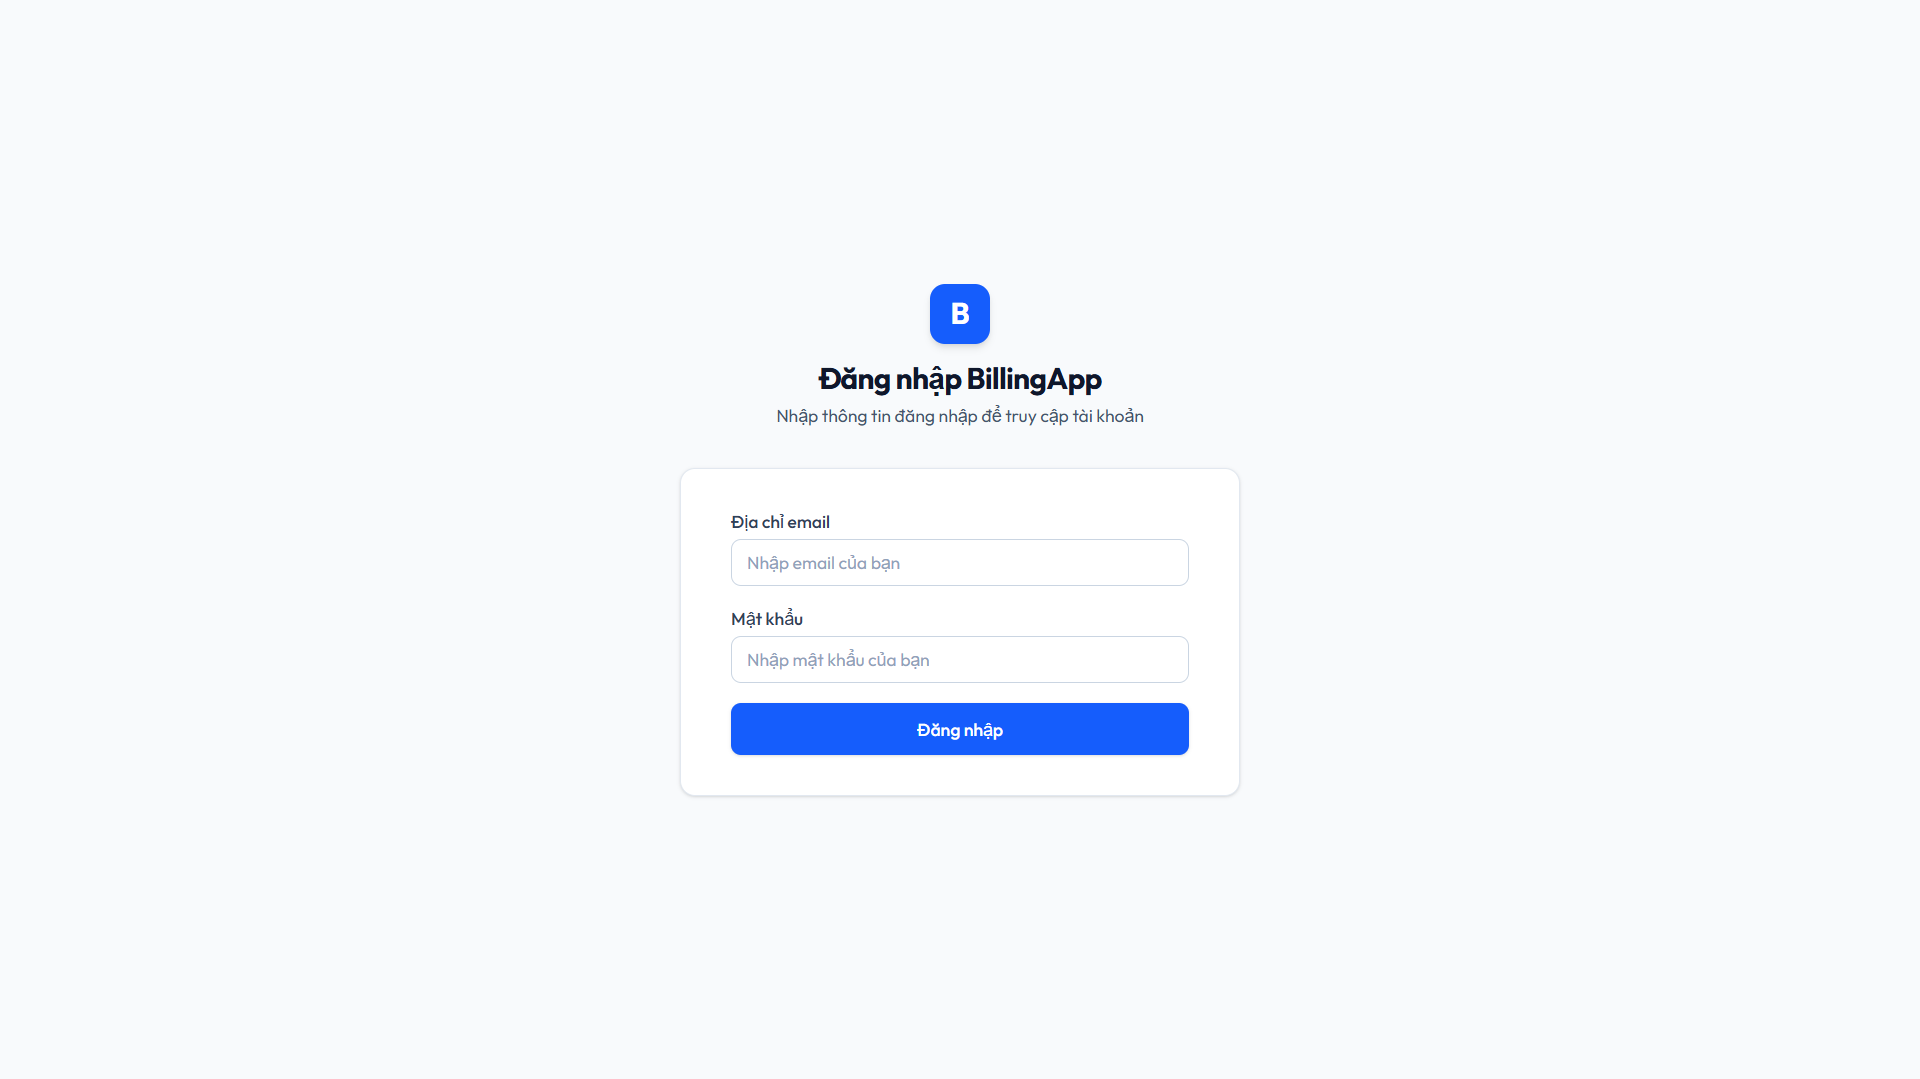
\includegraphics[width=0.75\textwidth]{images/ui_login.png}
}{
    \fbox{\parbox{0.9\textwidth}{\centering \vspace{15mm}
    \textbf{[HÌNH 3.1: GIAO DIỆN ĐĂNG NHẬP HỆ THỐNG (LOGIN VIEW)]}\\
    \textit{(Vị trí ảnh chụp: report/images/ui\_login.png)}\\
    \vspace{15mm}}}
}
\caption{Giao diện Đăng nhập và Xác thực người dùng (Auth Login)}
\label{fig:ui_login}
\end{figure}

\subsection{Màn hình Bán hàng nhanh (POS Checkout View)}
Màn hình Bán hàng nhanh (đường dẫn \texttt{/explore}) là giao diện làm việc chính của nhân viên thu ngân trong suốt ca bán (Hình \ref{fig:ui_pos_explore}):
\begin{itemize}[leftmargin=1.5cm]
    \item \textbf{Thanh phân loại danh mục (\texttt{DisplayCategories}):} Hiển thị danh sách các nhóm hàng dạng thẻ màu trực quan (như Cà phê, Trà sữa, Bánh ngọt), cho phép lọc nhanh sản phẩm theo nhóm chỉ với một cú nhấp.
    \item \textbf{Lưới hiển thị sản phẩm (\texttt{DisplayItems}):} Danh sách mặt hàng được bố trí dạng thẻ (Card) gồm hình ảnh đại diện từ AWS S3, tên mặt hàng, khoảng giá bán và số dư tồn kho khả dụng tức thời.
    \item \textbf{Thanh tìm kiếm thông minh (\texttt{SearchBox}):} Tích hợp hook tùy biến \texttt{useDebounce} (độ trễ $300$ms), hỗ trợ tìm kiếm sản phẩm theo tên hoặc quét trực tiếp mã vạch SKU bằng máy quét cầm tay.
\end{itemize}

\begin{figure}[H]
\centering
\IfFileExists{images/ui_pos_explore.png}{
    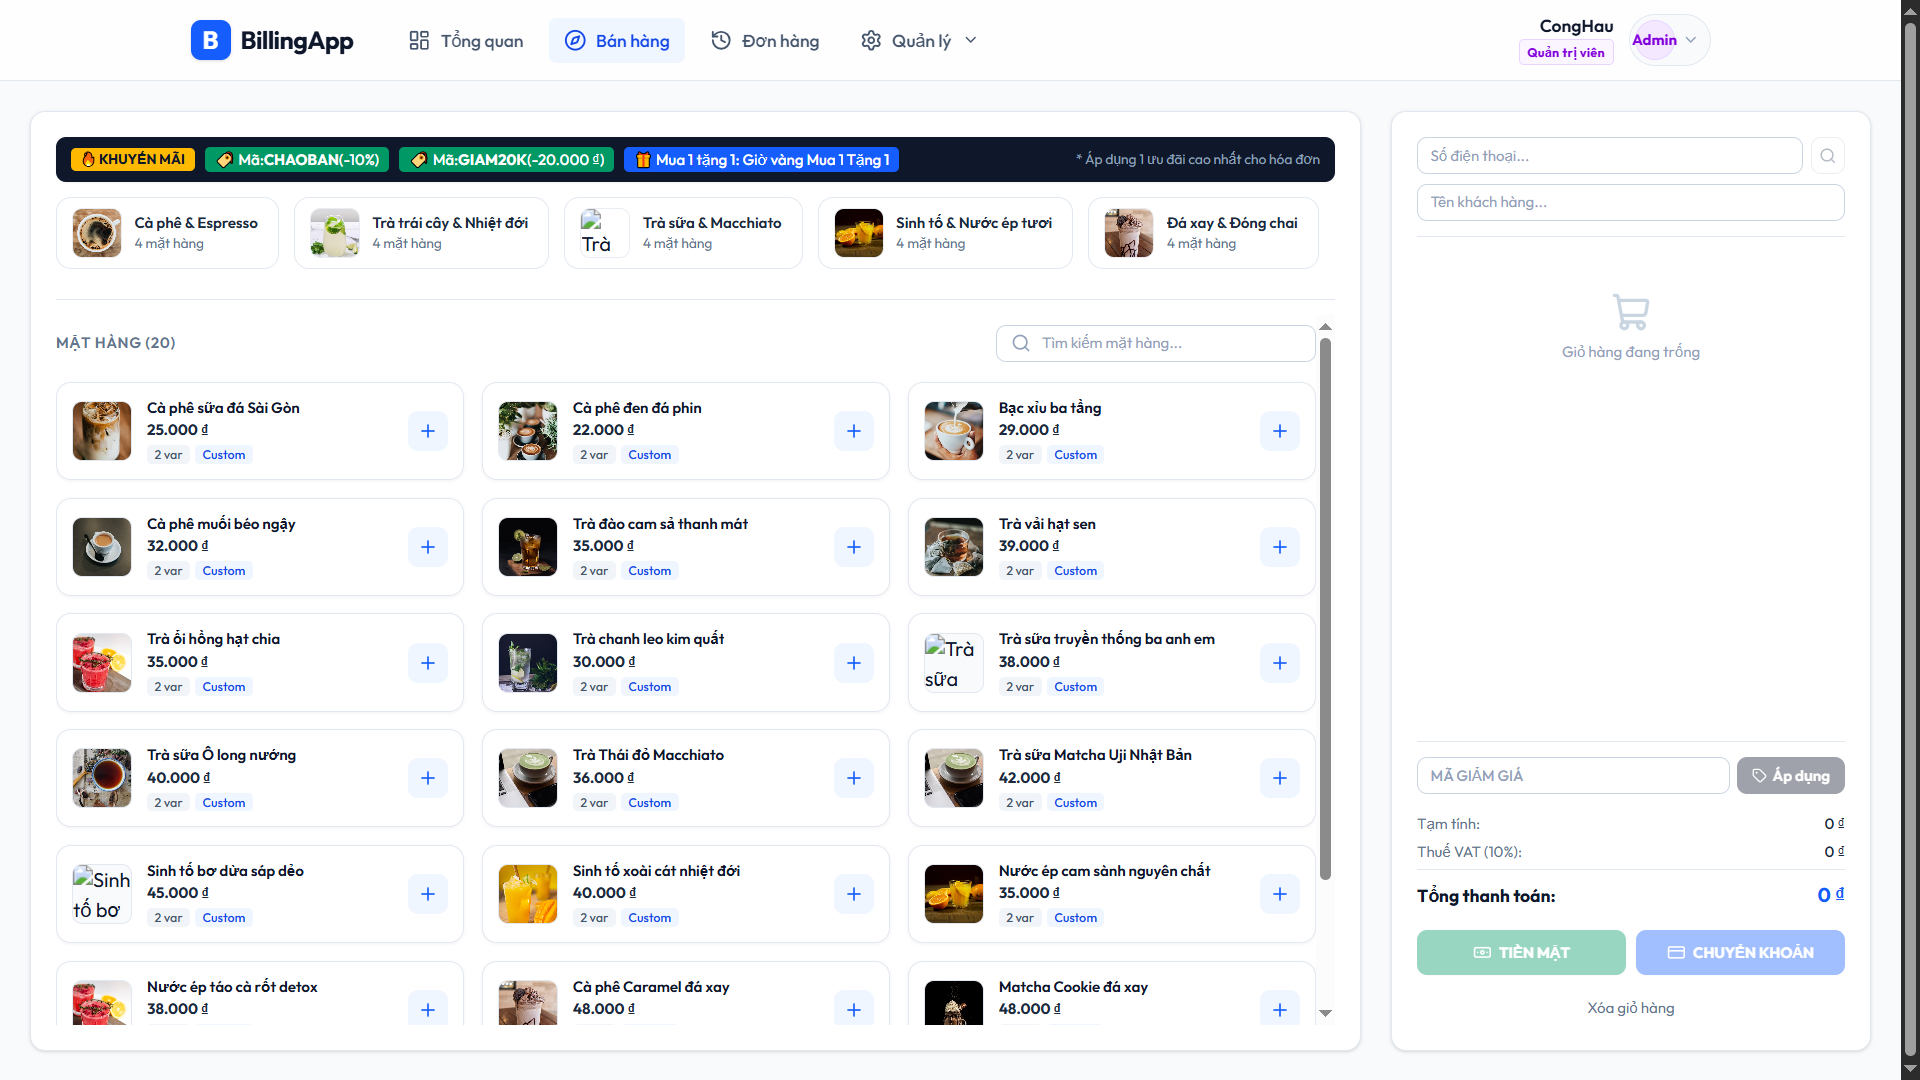
\includegraphics[width=0.92\textwidth]{images/ui_pos_explore.png}
}{
    \fbox{\parbox{0.9\textwidth}{\centering \vspace{15mm}
    \textbf{[HÌNH 3.2: GIAO DIỆN MÀN HÌNH BÁN HÀNG NHANH POS (EXPLORE VIEW)]}\\
    \textit{(Vị trí ảnh chụp: report/images/ui\_pos\_explore.png)}\\
    \vspace{15mm}}}
}
\caption{Giao diện Màn hình Bán hàng nhanh tại quầy POS}
\label{fig:ui_pos_explore}
\end{figure}

\subsection{Popup tùy biến Biến thể (Variants) và Nhóm tùy chọn (Modifiers)}
Khi thu ngân nhấp chọn một mặt hàng có cấu hình phân loại phức tạp, hệ thống mở cửa sổ con \texttt{POSItemModal} (Hình \ref{fig:ui_pos_modal}):
\begin{itemize}[leftmargin=1.5cm]
    \item \textbf{Lựa chọn biến thể SKU:} Thu ngân chọn kích thước (Size M/L) hoặc thuộc tính màu sắc. Hệ thống tự động cập nhật đơn giá cơ sở tương ứng và hiển thị số lượng hàng còn trong kho của biến thể đó.
    \item \textbf{Lựa chọn nhóm tùy chọn bổ sung (Modifiers):} Hiển thị các nhóm như Topping thêm, Mức đá, Mức đường. Hệ thống tự động kiểm tra các ràng buộc: số lượng chọn tối thiểu (\texttt{minSelections}) và tối đa (\texttt{maxSelections}). Khi chọn thêm Topping (ví dụ: Trân châu trắng +$10.000$đ), tổng giá tiền trên modal tự động cộng dồn theo thời gian thực.
    \item Nhấn nút ''Thêm vào giỏ hàng'', sản phẩm được đưa vào giỏ với mã định danh kết hợp duy nhất: \texttt{\$\{itemId\}\_\$\{variantId\}\_\$\{modifierIds\}}.
\end{itemize}

\begin{figure}[H]
\centering
\IfFileExists{images/ui_pos_modal.png}{
    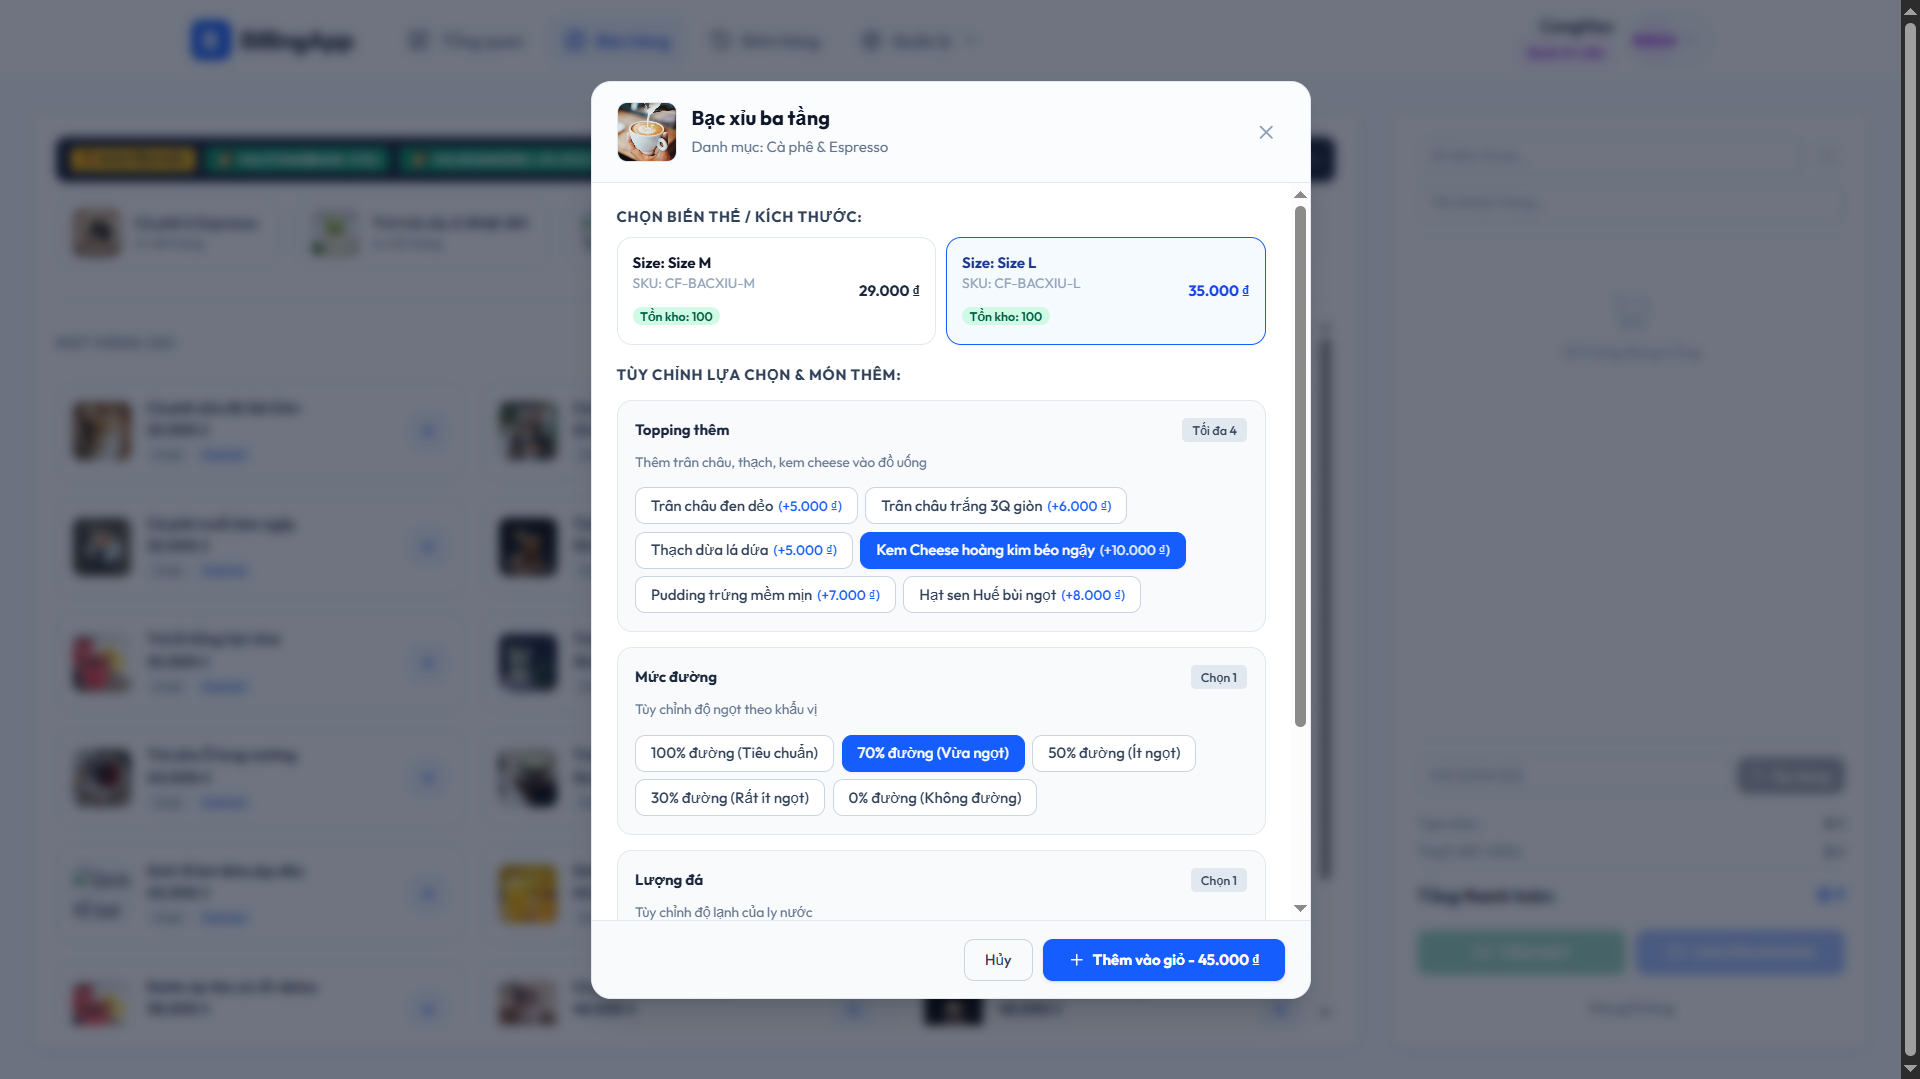
\includegraphics[width=0.88\textwidth]{images/ui_pos_modal.png}
}{
    \fbox{\parbox{0.9\textwidth}{\centering \vspace{12mm}
    \textbf{[HÌNH 3.3: POPUP TÙY CHỌN BIẾN THỂ SKU VÀ NHÓM TOPPING MODIFIERS]}\\
    \textit{(Vị trí ảnh chụp: report/images/ui\_pos\_modal.png)}\\
    \vspace{12mm}}}
}
\caption{Giao diện Popup tùy chọn biến thể SKU và Modifiers}
\label{fig:ui_pos_modal}
\end{figure}

\subsection{Quản lý Giỏ hàng và Nhận diện Khách hàng thân thiết CRM}
Bên phải màn hình bán hàng là bảng tóm tắt đơn hàng (\texttt{CartSummary}):
\begin{itemize}[leftmargin=1.5cm]
    \item Danh sách các dòng hàng đã chọn kèm số lượng, nút tăng/giảm nhanh (+/-) và nút xóa dòng hàng.
    \item \textbf{Biểu mẫu khách hàng thân thiết (\texttt{CustomerForm}):} Thu ngân nhập số điện thoại khách hàng. Hook gọi API \texttt{GET /customers/by-phone/\{phone\}}. Nếu khách hàng đã tồn tại, hệ thống hiển thị ngay tên khách hàng, tổng tiền tích lũy và số điểm thưởng. Nếu là khách hàng mới, hệ thống cho phép tạo nhanh tài khoản CRM ngay tại quầy mà không làm gián đoạn giỏ hàng.
    \item \textbf{Tự động đánh giá khuyến mãi:} Hệ thống liên tục gửi dữ liệu giỏ hàng tới endpoint \texttt{/promotions/evaluate} để áp dụng mức giảm giá cao nhất (Happy Hour hoặc Coupon) và hiển thị rõ ràng số tiền được giảm trừ.
\end{itemize}

\subsection{Thanh toán kép: Tiền mặt và VietQR PayOS thời gian thực}
Thu ngân có thể lựa chọn 1 trong 2 phương thức thanh toán linh hoạt:
\begin{enumerate}[label=\arabic*., leftmargin=1.5cm]
    \item \textbf{Thanh toán Tiền mặt (CASH):} Thu ngân nhập số tiền khách đưa (có các nút gợi ý tiền mặt nhanh: 50k, 100k, 200k, 500k). Hệ thống tự động tính toán số tiền thừa phải trả lại khách và mở ngay cửa sổ in hóa đơn bán lẻ.
    \item \textbf{Thanh toán chuyển khoản VietQR PayOS (PAYOS):}
    \begin{itemize}
        \item Hệ thống kích hoạt cửa sổ \texttt{PaymentQRCode} (Hình \ref{fig:ui_payment_qr}), hiển thị mã VietQR động theo chuẩn NAPAS có nhúng chính xác số tiền cần trả và mã đơn hàng đã được khóa bảo vệ.
        \item Front-end kích hoạt hook \texttt{usePolledOrderData} thăm dò tự động mỗi 3 giây. Ngay khi khách hàng chuyển khoản thành công và PayOS gửi Webhook, màn hình tự động chuyển sang trạng thái \texttt{COMPLETED}.
        \item \textbf{Quy trình chuyển sang tiền mặt (\textit{Switch to Cash}):} Nếu khách hàng gặp sự cố mạng di động, thu ngân có thể nhấn nút \textit{''Chuyển sang tiền mặt''}. Hệ thống gọi API hủy link PayOS và ghi nhận thanh toán tiền mặt tức thì.
    \end{itemize}
\end{enumerate}

\begin{figure}[H]
\centering
\IfFileExists{images/ui_payment_qr.png}{
    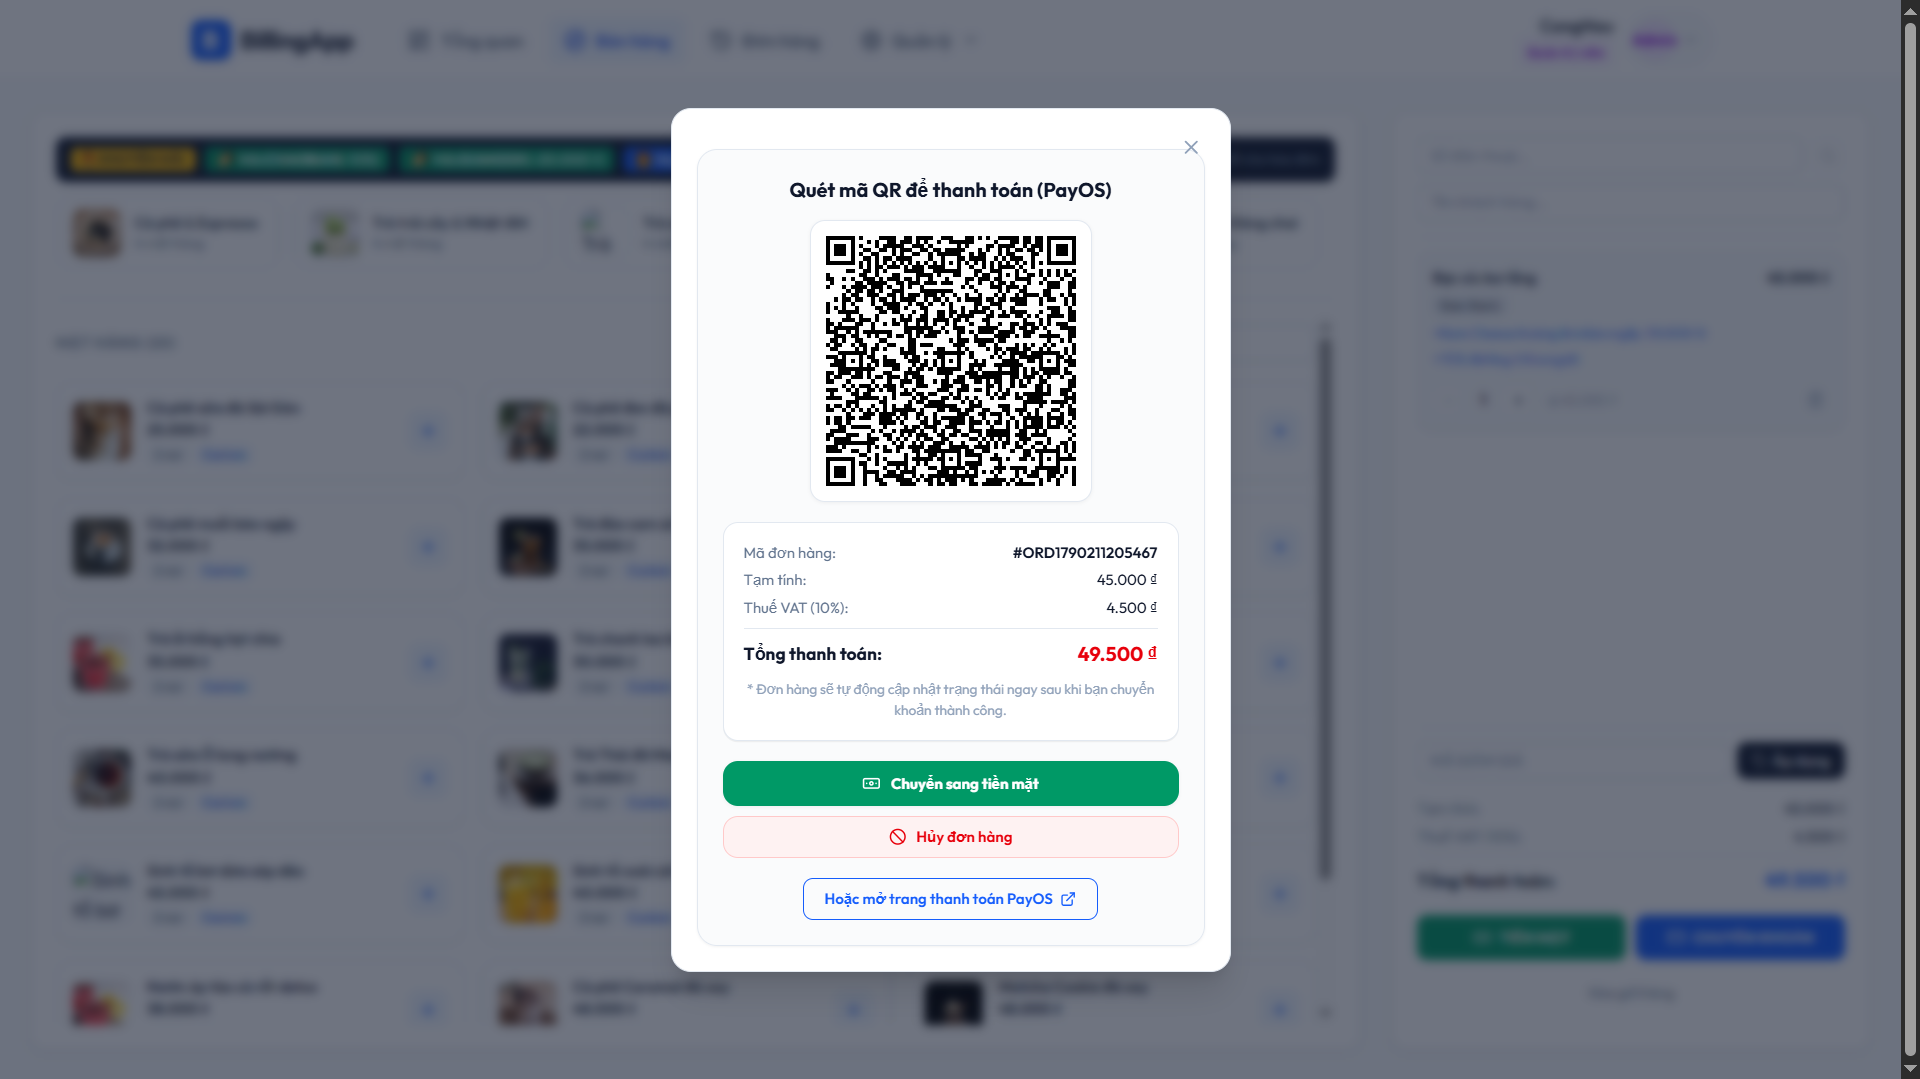
\includegraphics[width=0.88\textwidth]{images/ui_payment_qr.png}
}{
    \fbox{\parbox{0.9\textwidth}{\centering \vspace{15mm}
    \textbf{[HÌNH 3.4: CỬA SỔ QUÉT MÃ THANH TOÁN VIETQR PAYOS THỜI GIAN THỰC]}\\
    \textit{(Vị trí ảnh chụp: report/images/ui\_payment\_qr.png)}\\
    \vspace{15mm}}}
}
\caption{Giao diện Quét mã thanh toán VietQR động tích hợp PayOS}
\label{fig:ui_payment_qr}
\end{figure}

\subsection{Mẫu in hóa đơn bán lẻ nhiệt 80mm}
Cửa sổ \texttt{ReceiptPopup} (Hình \ref{fig:ui_receipt}) được thiết kế chuẩn mực theo tiêu chuẩn giấy in nhiệt 80mm thông dụng tại các siêu thị và nhà hàng:
\begin{itemize}[leftmargin=1.5cm]
    \item Phần đầu: Tên cửa hàng, địa chỉ, số điện thoại hotline và số hiệu hóa đơn (\texttt{order\_code}).
    \item Phần thân: Bảng danh sách các mặt hàng, biến thể SKU, danh sách Modifier đính kèm, số lượng, đơn giá và thành tiền.
    \item Phần chân: Tổng tiền hàng (\texttt{subtotal}), tiền chiết khấu khuyến mãi (\texttt{discountAmount}), tiền thuế VAT 10\% (\texttt{tax}), tổng thanh toán cuối cùng (\texttt{grandTotal}), phương thức thanh toán, tiền khách đưa và tiền thừa thối lại.
    \item Tích hợp lệnh gọi in trực tiếp trình duyệt (\texttt{window.print()}) với định dạng \texttt{@media print} tối ưu độ sắc nét cho đầu in nhiệt.
\end{itemize}

\begin{figure}[H]
\centering
\IfFileExists{images/ui_receipt.png}{
    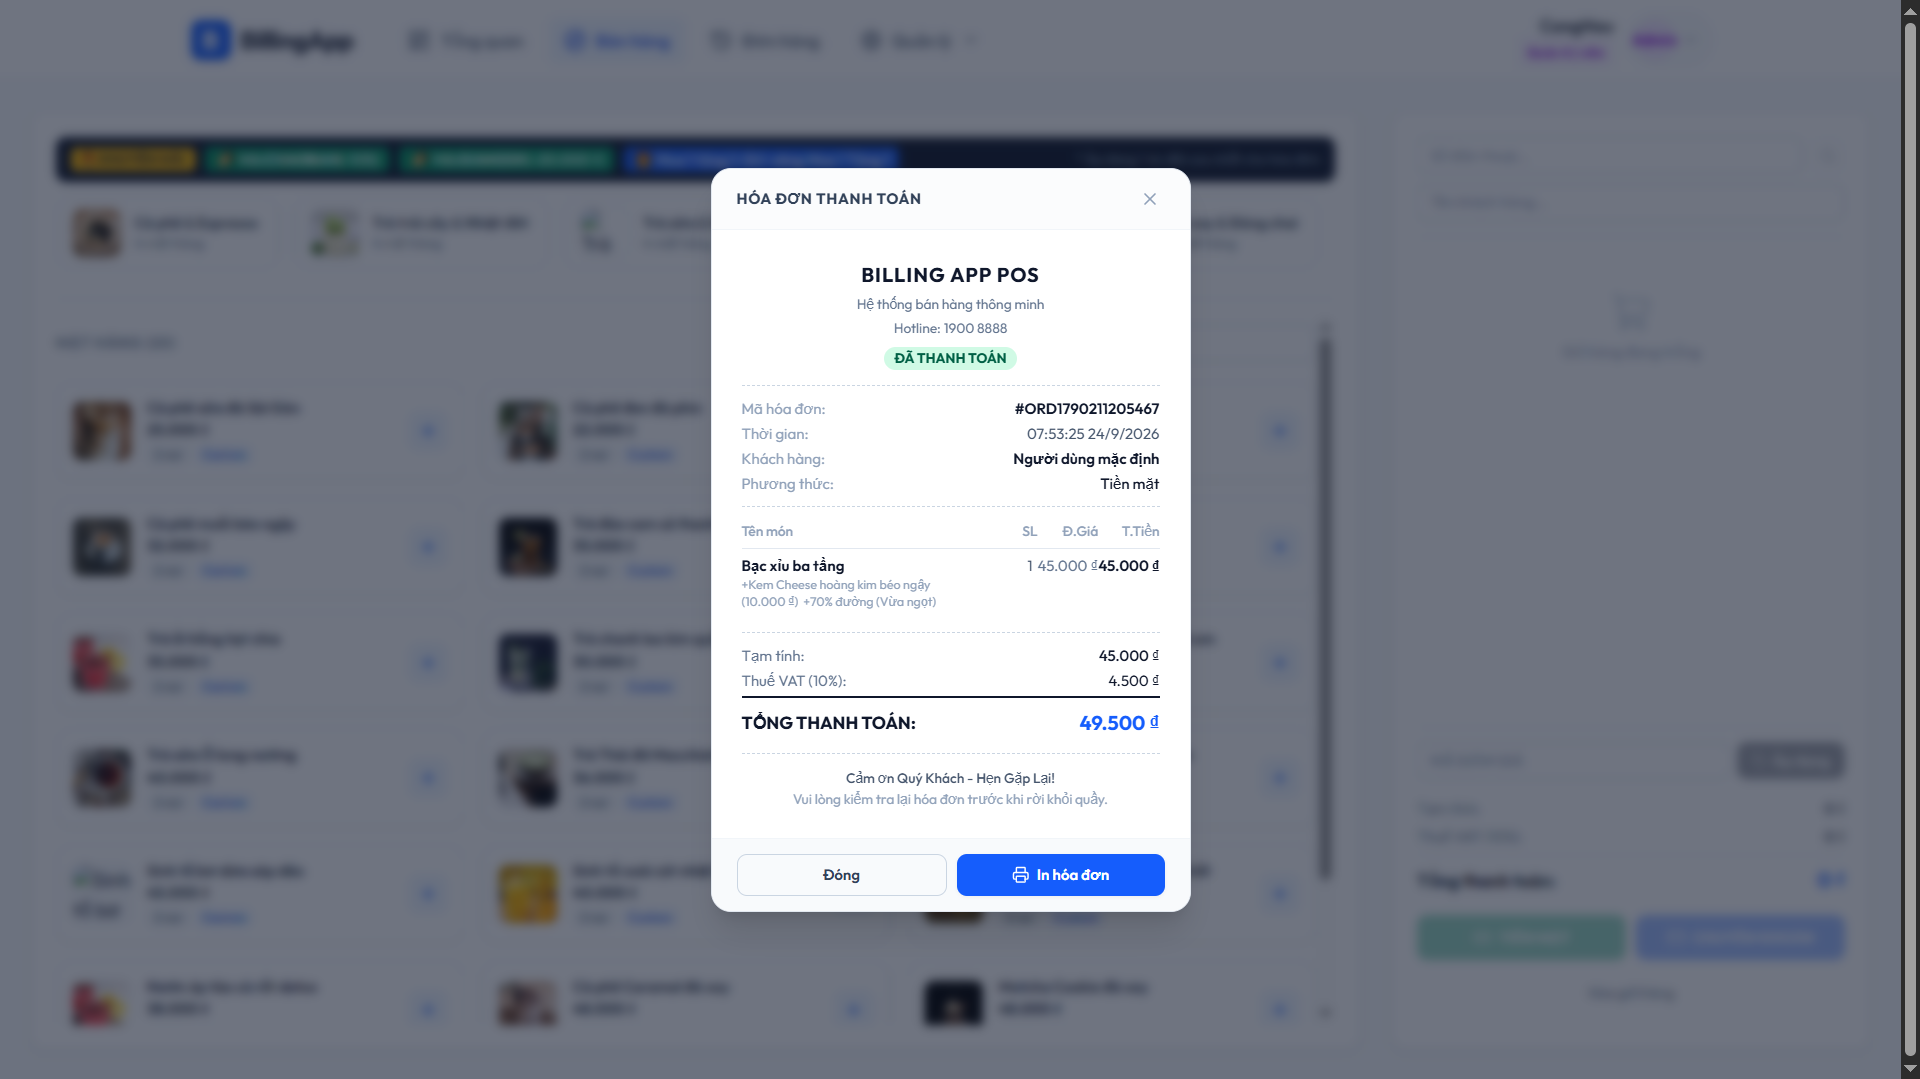
\includegraphics[width=0.85\textwidth]{images/ui_receipt.png}
}{
    \fbox{\parbox{0.9\textwidth}{\centering \vspace{15mm}
    \textbf{[HÌNH 3.5: MẪU HÓA ĐƠN BÁN LẺ IN NHIỆT 80MM (THERMAL RECEIPT)]}\\
    \textit{(Vị trí ảnh chụp: report/images/ui\_receipt.png)}\\
    \vspace{15mm}}}
}
\caption{Mẫu Hóa đơn bán lẻ in nhiệt 80mm chuẩn hóa}
\label{fig:ui_receipt}
\end{figure}

\subsection{Màn hình Lịch sử đơn hàng và Hủy đơn bù trừ kho}
Màn hình Lịch sử đơn hàng (\texttt{OrderHistory} - Hình \ref{fig:ui_order_history}) cung cấp các công cụ quản lý sau bán hàng:
\begin{itemize}[leftmargin=1.5cm]
    \item Danh sách phân trang toàn bộ các hóa đơn đã phát sinh, hỗ trợ bộ lọc theo trạng thái: \texttt{PENDING}, \texttt{COMPLETED}, \texttt{CANCELLED}.
    \item Xem lại chi tiết đơn hàng và in lại hóa đơn (Re-print receipt) bất kỳ lúc nào.
    \item \textbf{Cơ chế bảo vệ kế toán nghiêm ngặt:} Đơn hàng đã \texttt{COMPLETED} không có nút xóa nhằm chống gian lận doanh số. Nút ''Hủy đơn'' chỉ xuất hiện đối với đơn hàng đang \texttt{PENDING}. Khi xác nhận hủy, hệ thống kích hoạt giao dịch bù trừ kho (Stock In) và hoàn lại số lượt dùng voucher khuyến mãi.
\end{itemize}

\begin{figure}[H]
\centering
\IfFileExists{images/ui_order_history.png}{
    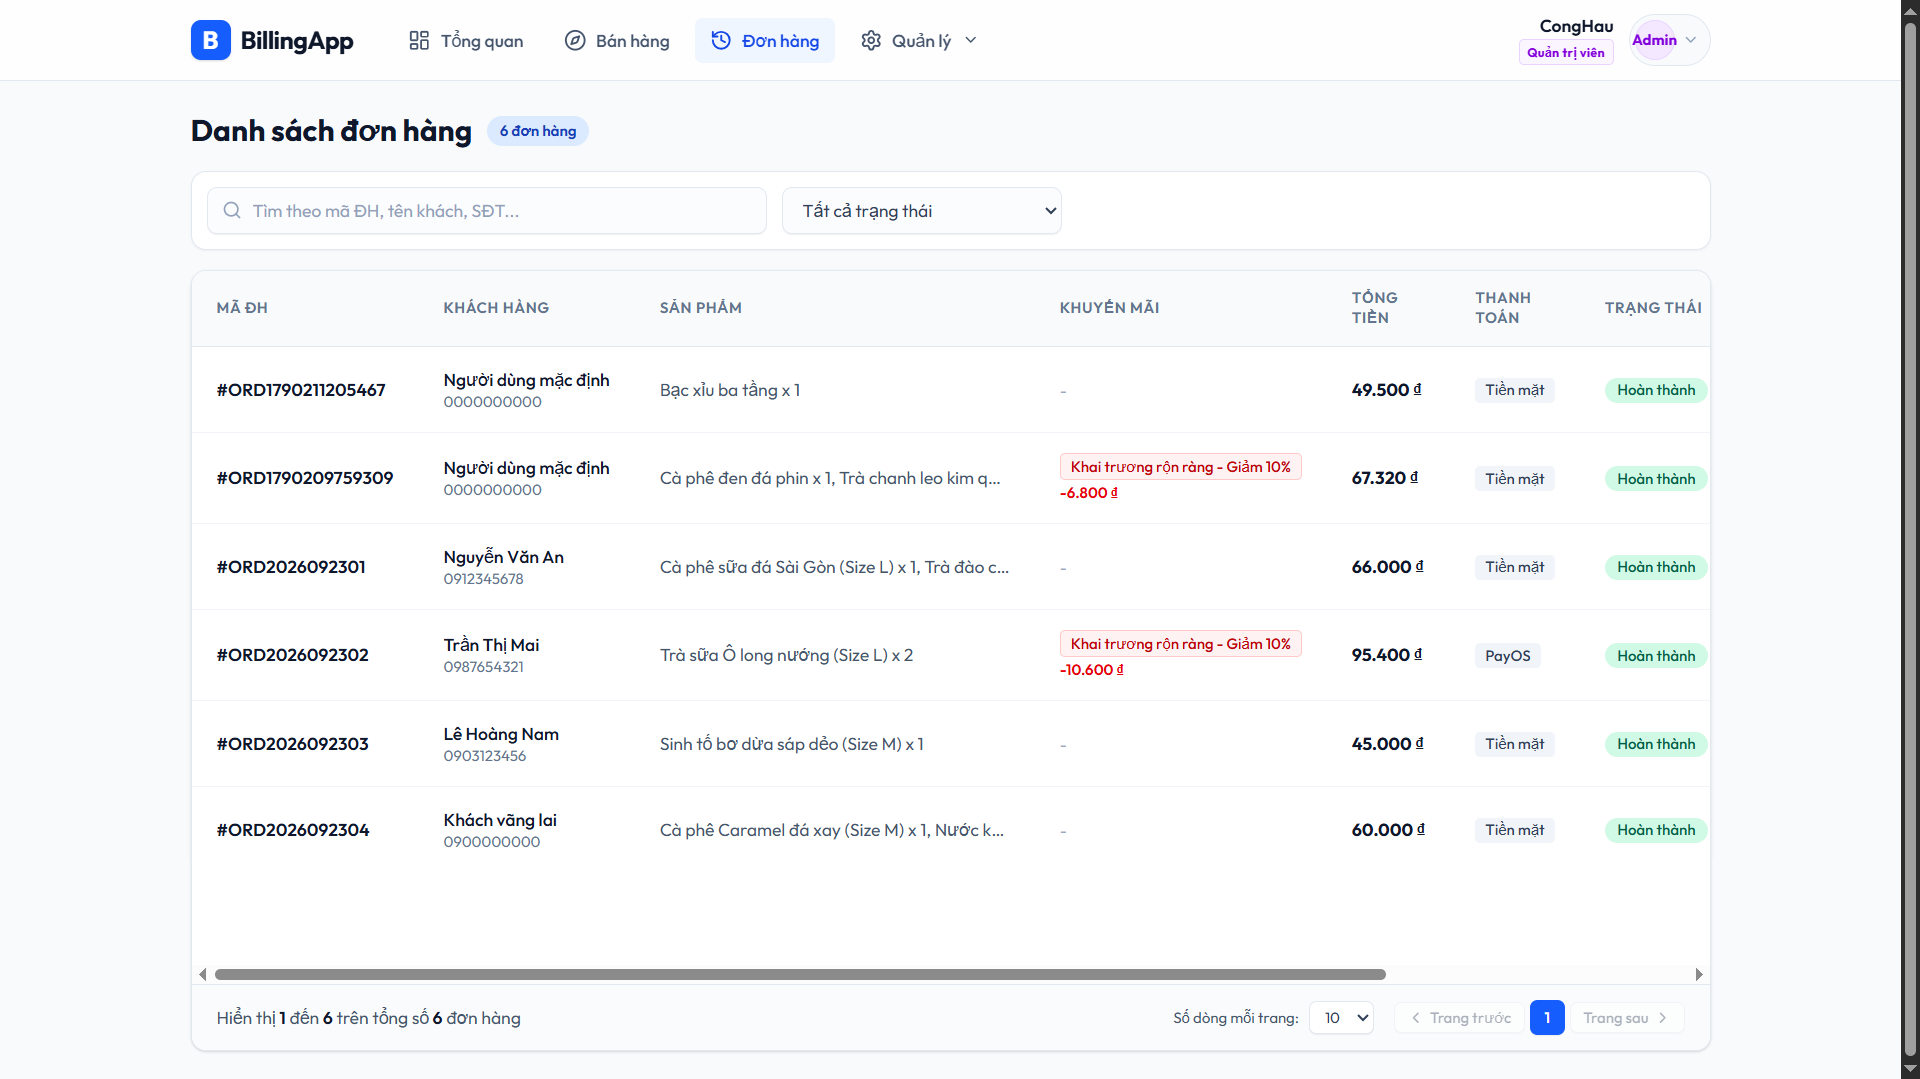
\includegraphics[width=0.92\textwidth]{images/ui_order_history.png}
}{
    \fbox{\parbox{0.9\textwidth}{\centering \vspace{15mm}
    \textbf{[HÌNH 3.6: GIAO DIỆN LỊCH SỬ ĐƠN HÀNG VÀ THEO DÕI TRẠNG THÁI]}\\
    \textit{(Vị trí ảnh chụp: report/images/ui\_order\_history.png)}\\
    \vspace{15mm}}}
}
\caption{Giao diện Quản lý Lịch sử đơn hàng và Trạng thái thanh toán}
\label{fig:ui_order_history}
\end{figure}

% ==============================================================================
\section{Hiện thực phân hệ Quản trị (Dành cho Admin/Quản lý)}
\label{sec:hien_thuc_quan_tri}

Phân hệ Quản trị được bảo vệ bởi bộ định tuyến an ninh \texttt{AdminRoute}, chỉ cho phép tài khoản có vai trò \texttt{ROLE\_ADMIN} truy cập.

\subsection{Bảng điều khiển chỉ số kinh doanh và Báo cáo Doanh thu (Dashboard KPI)}
Trang chủ Quản trị (\texttt{/dashboard} - Hình \ref{fig:ui_dashboard}) cung cấp bức tranh toàn cảnh về hiệu quả kinh doanh của cửa hàng trong ngày và hỗ trợ báo cáo thống kê doanh thu chuyên sâu:
\begin{itemize}[leftmargin=1.5cm]
    \item \textbf{Thẻ đo lường KPI doanh thu:} Tổng doanh thu ngày/tuần/tháng hiện tại, tỉ lệ tăng trưởng so với kỳ trước cùng khoảng thời gian, biểu thị bằng mũi tên xu hướng tăng/giảm kèm phần trăm.
    \item \textbf{Thẻ đếm số lượng hóa đơn:} Tổng số đơn hàng hoàn tất (\texttt{COMPLETED}), số đơn đang chờ (\texttt{PENDING}) và số đơn đã hủy (\texttt{CANCELLED}) trong khoảng thời gian.
    \item \textbf{Bảng danh sách đơn hàng mới nhất:} Hiển thị các giao dịch vừa phát sinh theo thời gian thực kèm mã hóa đơn và trạng thái thanh toán.
    \item \textbf{Bảng xếp hạng sản phẩm bán chạy (Top Items):} Danh sách các sản phẩm có số lượng bán cao nhất, tổng hợp từ bảng \texttt{tbl\_order\_items} theo biến thể SKU.
    \item \textbf{Cảnh báo tồn kho thấp (Low Stock Alert):} Liệt kê các biến thể có số dư \texttt{cachedStockQuantity} dưới ngưỡng cảnh báo, giúp quản lý chủ động lên kế hoạch nhập hàng kịp thời.
\end{itemize}

\begin{figure}[H]
\centering
\IfFileExists{images/ui_dashboard.png}{
    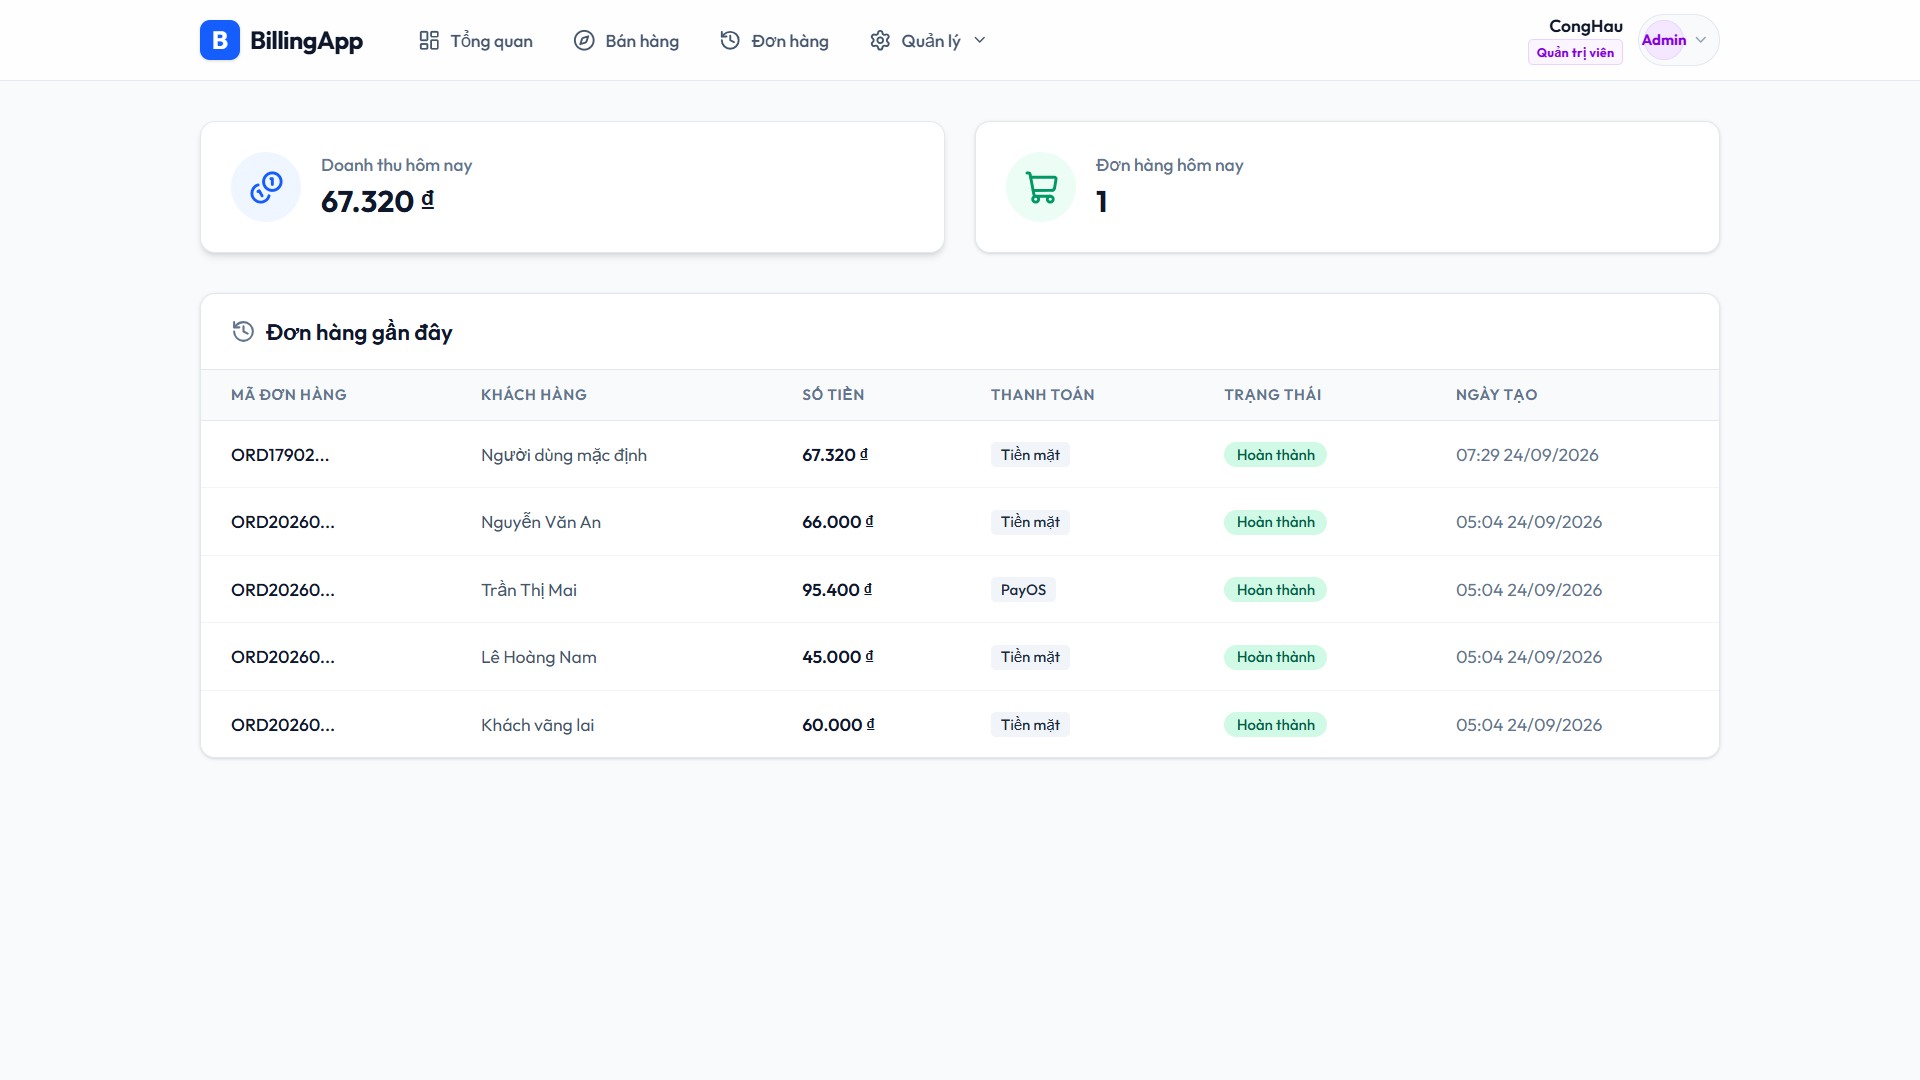
\includegraphics[width=0.92\textwidth]{images/ui_dashboard.png}
}{
    \fbox{\parbox{0.9\textwidth}{\centering \vspace{15mm}
    \textbf{[HÌNH 3.7: BẢNG ĐIỀU KHIỂN CHỈ SỐ KINH DOANH VÀ BÁO CÁO DOANH THU (DASHBOARD)]}\\
    \textit{(Vị trí ảnh chụp: report/images/ui\_dashboard.png)}\\
    \vspace{15mm}}}
}
\caption{Giao diện Bảng điều khiển kinh doanh tổng quan và Báo cáo Doanh thu (Dashboard)}
\label{fig:ui_dashboard}
\end{figure}

\subsection{Quản trị Danh mục hàng hóa (Categories)}
Giao diện Quản trị Danh mục (\texttt{/categories} - Hình \ref{fig:ui_manage_categories}) cho phép người quản lý tổ chức cây danh mục mặt hàng theo từng nhóm nghiệp vụ:
\begin{itemize}[leftmargin=1.5cm]
    \item Danh sách phân loại các nhóm sản phẩm (Cà phê, Trà hoa quả, Đồ ăn nhanh, Bánh ngọt).
    \item Thêm mới, cập nhật tên danh mục, biểu tượng nhận diện và trạng thái kích hoạt hiển thị tại quầy POS.
    \item Ràng buộc toàn vẹn: Không cho phép xóa danh mục khi đang có sản phẩm con liên kết (\texttt{ON DELETE RESTRICT}).
\end{itemize}

\begin{figure}[H]
\centering
\IfFileExists{images/ui_manage_categories.png}{
    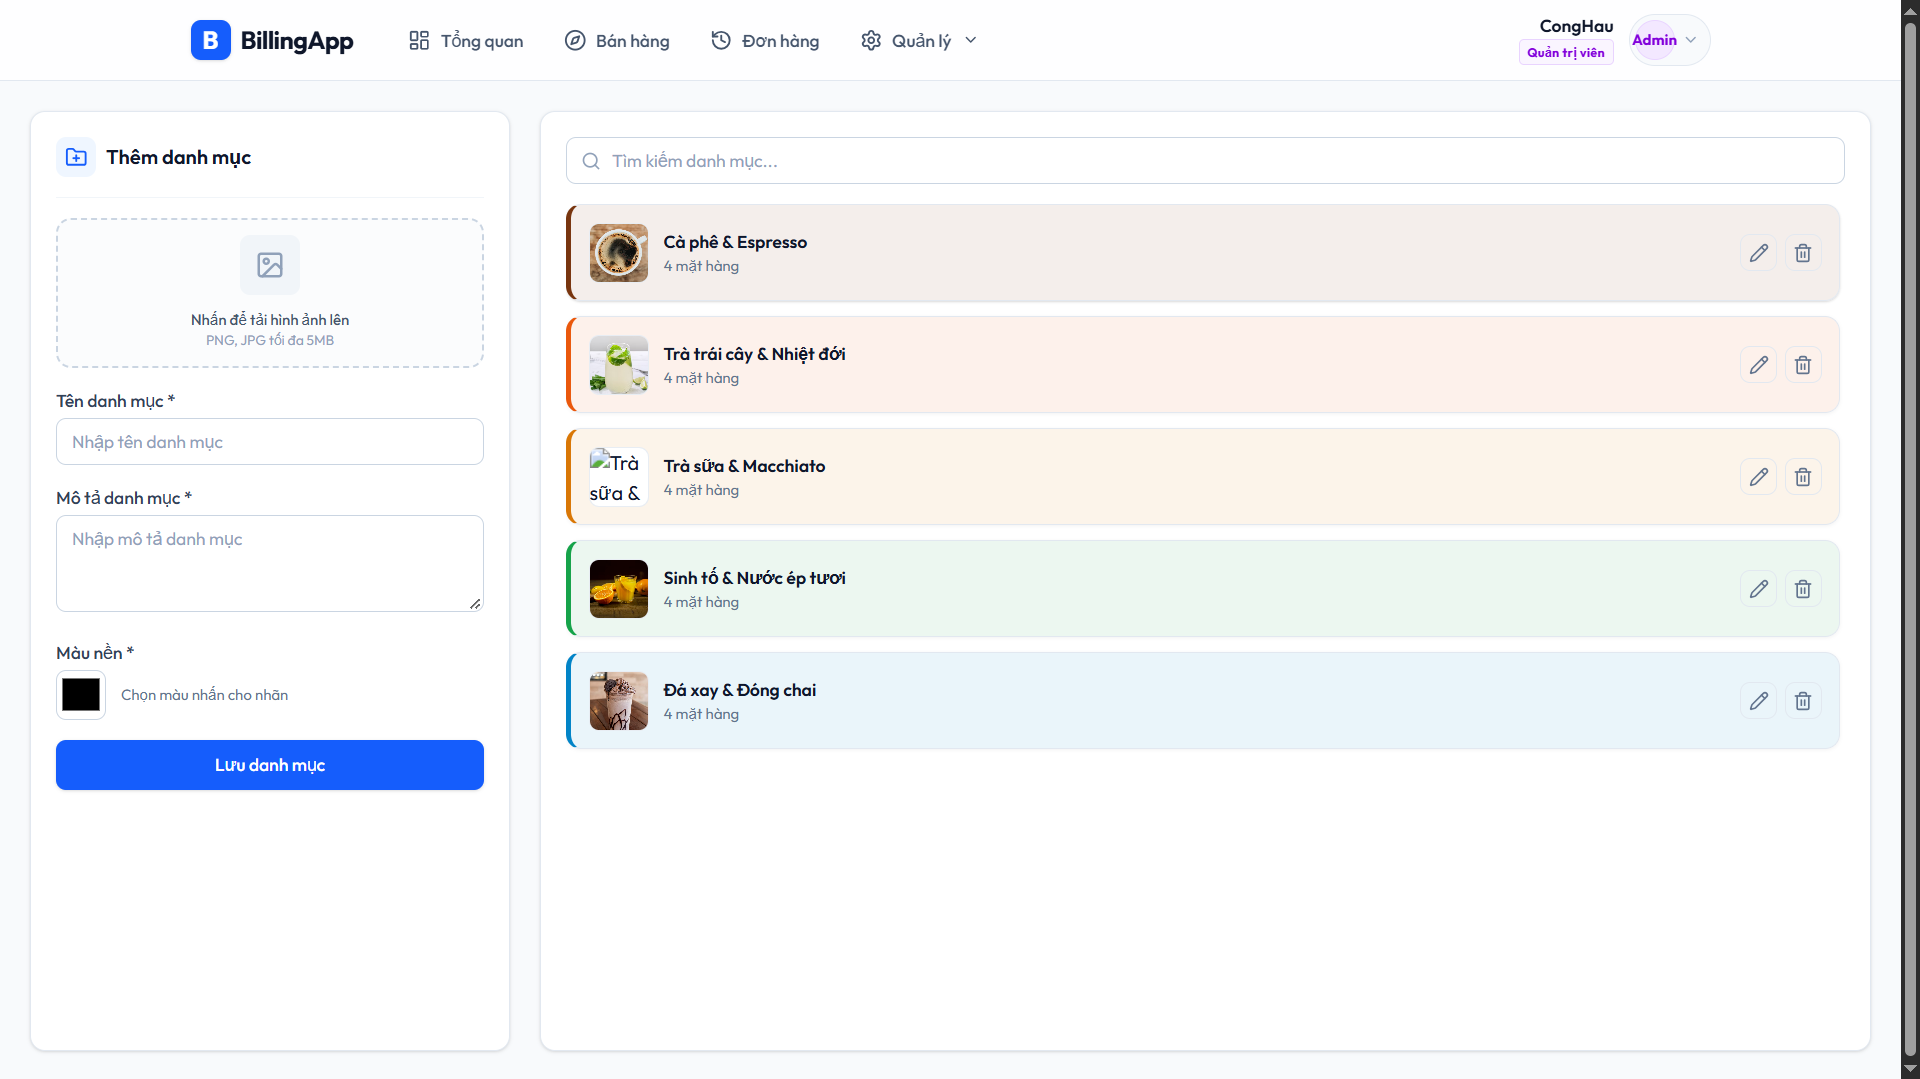
\includegraphics[width=0.92\textwidth]{images/ui_manage_categories.png}
}{
    \fbox{\parbox{0.9\textwidth}{\centering \vspace{15mm}
    \textbf{[HÌNH 3.8: GIAO DIỆN QUẢN TRỊ DANH MỤC HÀNG HÓA]}\\
    \textit{(Vị trí ảnh chụp: report/images/ui\_manage\_categories.png)}\\
    \vspace{15mm}}}
}
\caption{Giao diện Quản trị Danh mục hàng hóa (Categories)}
\label{fig:ui_manage_categories}
\end{figure}

\subsection{Quản lý Sản phẩm, Biến thể SKU và Tải ảnh AWS S3}
Trang Quản lý Sản phẩm (\texttt{/items} - Hình \ref{fig:ui_manage_items}) hỗ trợ:
\begin{itemize}[leftmargin=1.5cm]
    \item Thêm mới và cập nhật sản phẩm có kèm tệp hình ảnh tải lên kho đám mây AWS S3.
    \item Tạo động danh sách các biến thể phân loại (SKU) với bảng thuộc tính động dạng JSON (như Size: L, Màu: Đỏ).
    \item Gán các nhóm tùy chọn Modifier vào từng sản phẩm tương ứng.
\end{itemize}

\begin{figure}[H]
\centering
\IfFileExists{images/ui_manage_items.png}{
    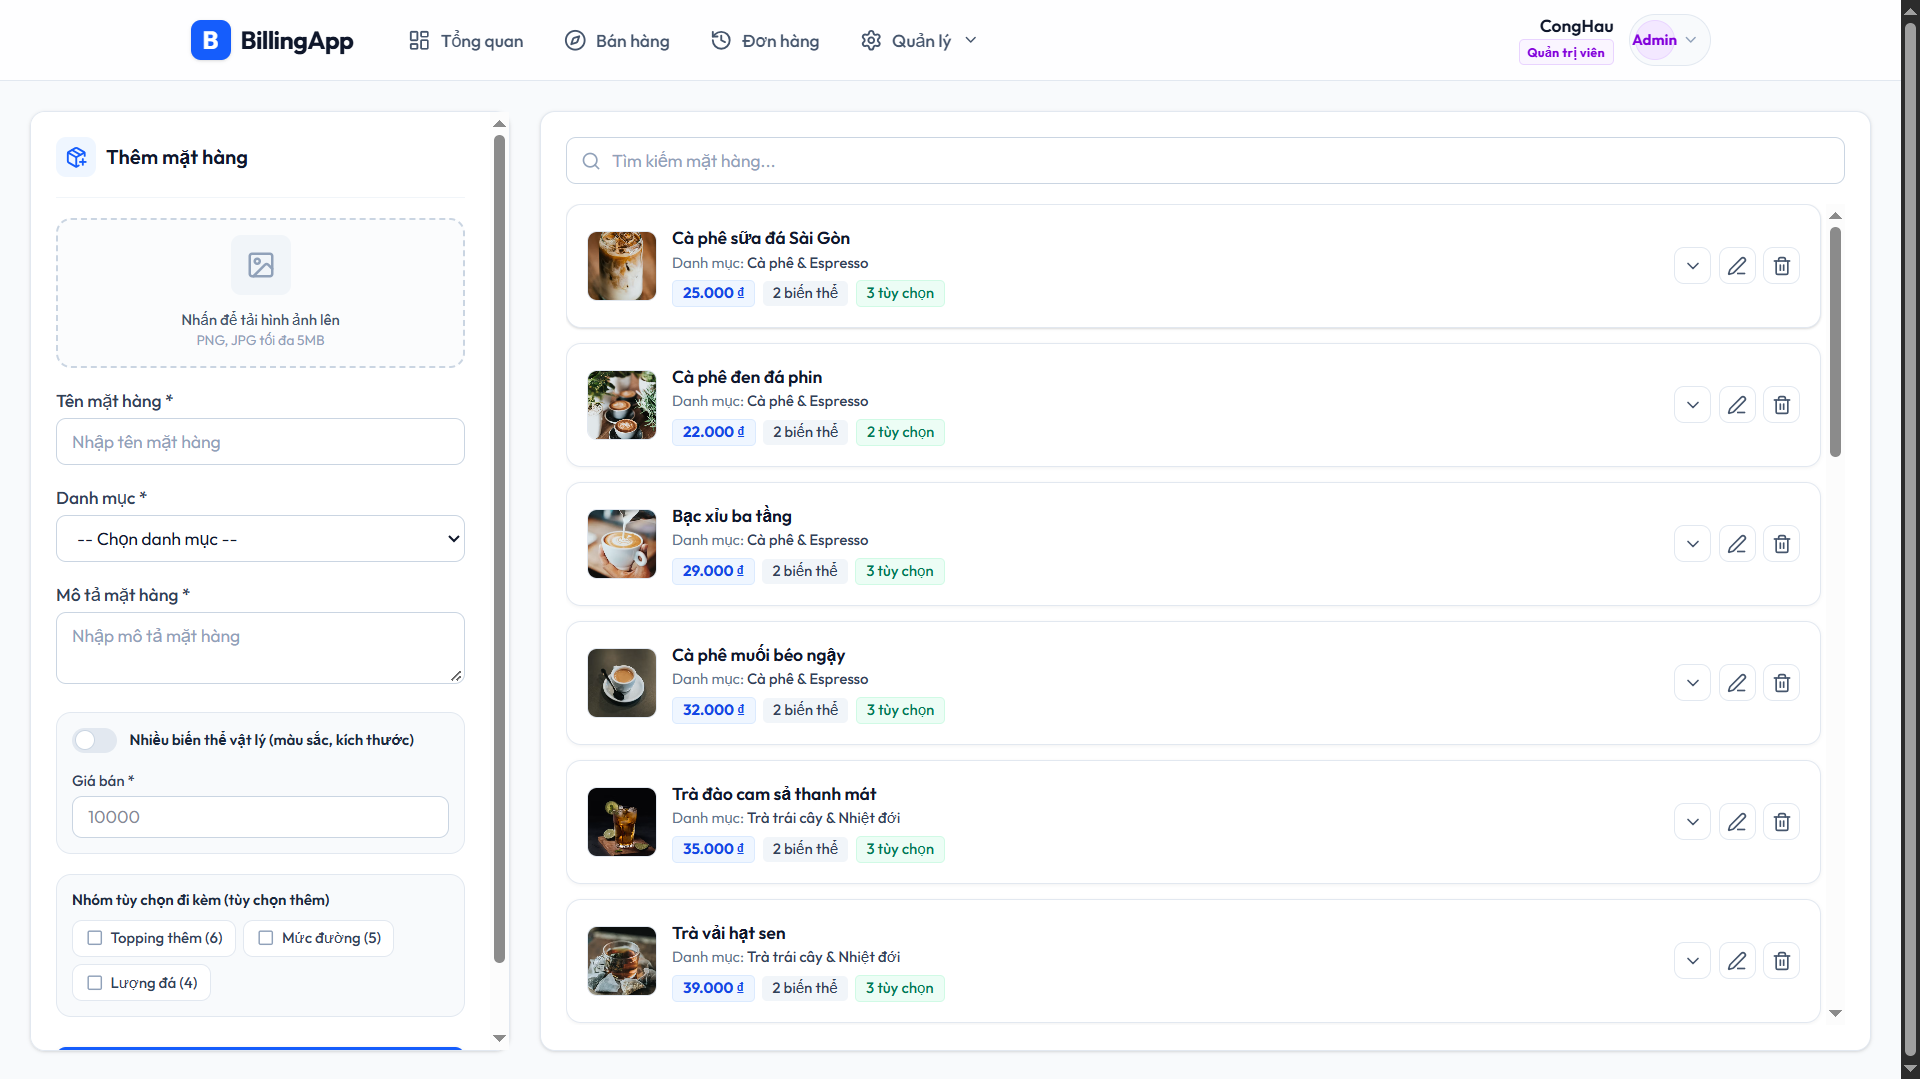
\includegraphics[width=0.92\textwidth]{images/ui_manage_items.png}
}{
    \fbox{\parbox{0.9\textwidth}{\centering \vspace{15mm}
    \textbf{[HÌNH 3.9: GIAO DIỆN QUẢN LÝ SẢN PHẨM VÀ CÁC BIẾN THỂ PHÂN LOẠI]}\\
    \textit{(Vị trí ảnh chụp: report/images/ui\_manage\_items.png)}\\
    \vspace{15mm}}}
}
\caption{Giao diện Quản lý danh mục Sản phẩm và Biến thể SKU}
\label{fig:ui_manage_items}
\end{figure}

\subsection{Quản trị Nhóm tùy chọn bổ sung (Modifiers)}
Giao diện Quản lý Nhóm tùy chọn (\texttt{/modifiers} - Hình \ref{fig:ui_manage_modifiers}) hỗ trợ định nghĩa các nhóm phụ phí và gia giảm:
\begin{itemize}[leftmargin=1.5cm]
    \item Thiết lập các nhóm như Topping thêm, Mức đá (0\%, 50\%, 100\%), Mức đường (0\%, 30\%, 70\%, 100\%).
    \item Cấu hình số lựa chọn tối thiểu (\texttt{minSelections}) và tối đa (\texttt{maxSelections}).
    \item Danh sách các tùy chọn chi tiết bên trong nhóm kèm mức điều chỉnh giá (\texttt{priceAdjustment}).
\end{itemize}

\begin{figure}[H]
\centering
\IfFileExists{images/ui_manage_modifiers.png}{
    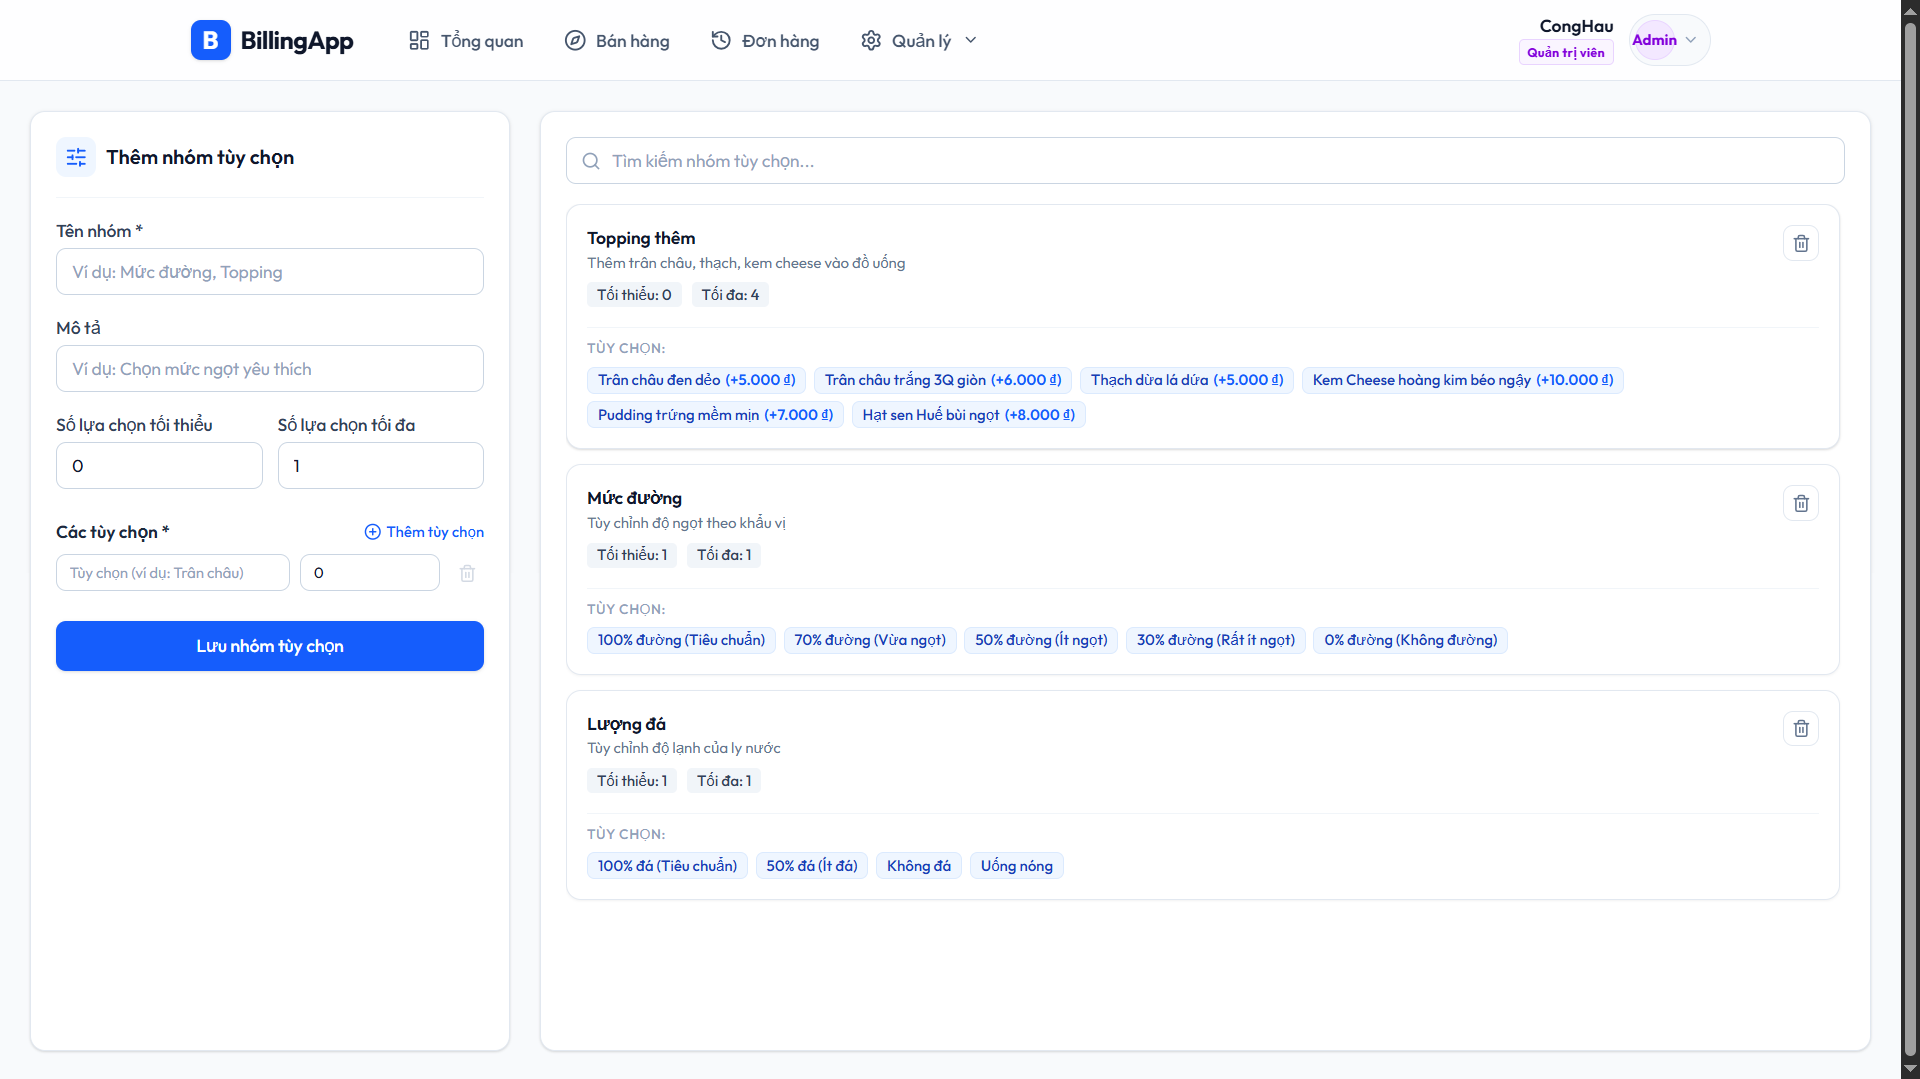
\includegraphics[width=0.92\textwidth]{images/ui_manage_modifiers.png}
}{
    \fbox{\parbox{0.9\textwidth}{\centering \vspace{15mm}
    \textbf{[HÌNH 3.10: GIAO DIỆN QUẢN TRỊ NHÓM TÙY CHỌN BỔ SUNG (MODIFIERS)]}\\
    \textit{(Vị trí ảnh chụp: report/images/ui\_manage\_modifiers.png)}\\
    \vspace{15mm}}}
}
\caption{Giao diện Quản trị Nhóm tùy chọn bổ sung (Modifiers)}
\label{fig:ui_manage_modifiers}
\end{figure}

\subsection{Quản lý Kho sổ cái và Kiểm kê cân bằng tồn kho}
Cửa sổ \texttt{StockOperationModal} (Hình \ref{fig:ui_stock_operation}) cung cấp các công cụ quản lý kho chuyên nghiệp:
\begin{itemize}[leftmargin=1.5cm]
    \item \textbf{Nhập kho (Stock IN):} Tăng số dư kho khi nhập lô hàng mới từ nhà cung cấp kèm mã phiếu nhập và ghi chú.
    \item \textbf{Xuất hủy (Stock OUT):} Giảm số dư kho khi xảy ra hư hỏng, hết hạn sử dụng hoặc thất thoát.
    \item \textbf{Kiểm kê kho (Stock Check):} Nhập số lượng đếm thực tế; hệ thống tự động suy ra số chênh lệch $\Delta$ và tạo giao dịch điều chỉnh \texttt{ADJUSTMENT}.
    \item \textbf{Xem sổ cái giao dịch:} Liệt kê toàn bộ lịch sử biến động kho theo dòng thời gian.
\end{itemize}

\begin{figure}[H]
\centering
\IfFileExists{images/ui_stock_operation.png}{
    \includegraphics[width=0.92\textwidth]{images/ui_stock_operation.png}
}{
    \fbox{\parbox{0.9\textwidth}{\centering \vspace{15mm}
    \textbf{[HÌNH 3.11: POPUP THAO TÁC SỔ CÁI KHO VÀ KIỂM KÊ CÂN BẰNG TỒN KHO]}\\
    \textit{(Vị trí ảnh chụp: report/images/ui\_stock\_operation.png)}\\
    \vspace{15mm}}}
}
\caption{Giao diện Popup Quản lý Sổ cái kho và Kiểm kê thực tế}
\label{fig:ui_stock_operation}
\end{figure}

\subsection{Quản lý Khuyến mãi, Khách hàng CRM và Tài khoản nhân viên}
Các màn hình quản trị bổ trợ gồm:
\begin{itemize}[leftmargin=1.5cm]
    \item \textbf{Quản lý Khuyến mãi (\texttt{/promotions} - Hình \ref{fig:ui_manage_promotions}):} Thiết lập các chương trình Coupon, Happy Hour, BOGO; hỗ trợ bật/tắt nhanh trạng thái kích hoạt (\texttt{toggleActive}).
    \item \textbf{Quản lý Khách hàng CRM (\texttt{/customers} - Hình \ref{fig:ui_manage_customers}):} Tra cứu danh bạ khách hàng, theo dõi lịch sử doanh số tích lũy và số lượng hóa đơn đã mua.
    \item \textbf{Quản lý Người dùng (\texttt{/users} - Hình \ref{fig:ui_manage_users}):} Cấp tài khoản nhân viên mới, cập nhật mật khẩu và gán vai trò quyền hạn (\texttt{ROLE\_ADMIN} vs \texttt{ROLE\_STAFF}).
    \item \textbf{Nhật ký Kiểm toán Hoạt động (\texttt{/activity-logs} - Hình \ref{fig:ui_activity_logs}):} Tra cứu và lọc lịch sử thao tác của các tài khoản trong hệ thống phục vụ công tác đối soát an ninh.
\end{itemize}

\begin{figure}[H]
\centering
\IfFileExists{images/ui_manage_promotions.png}{
    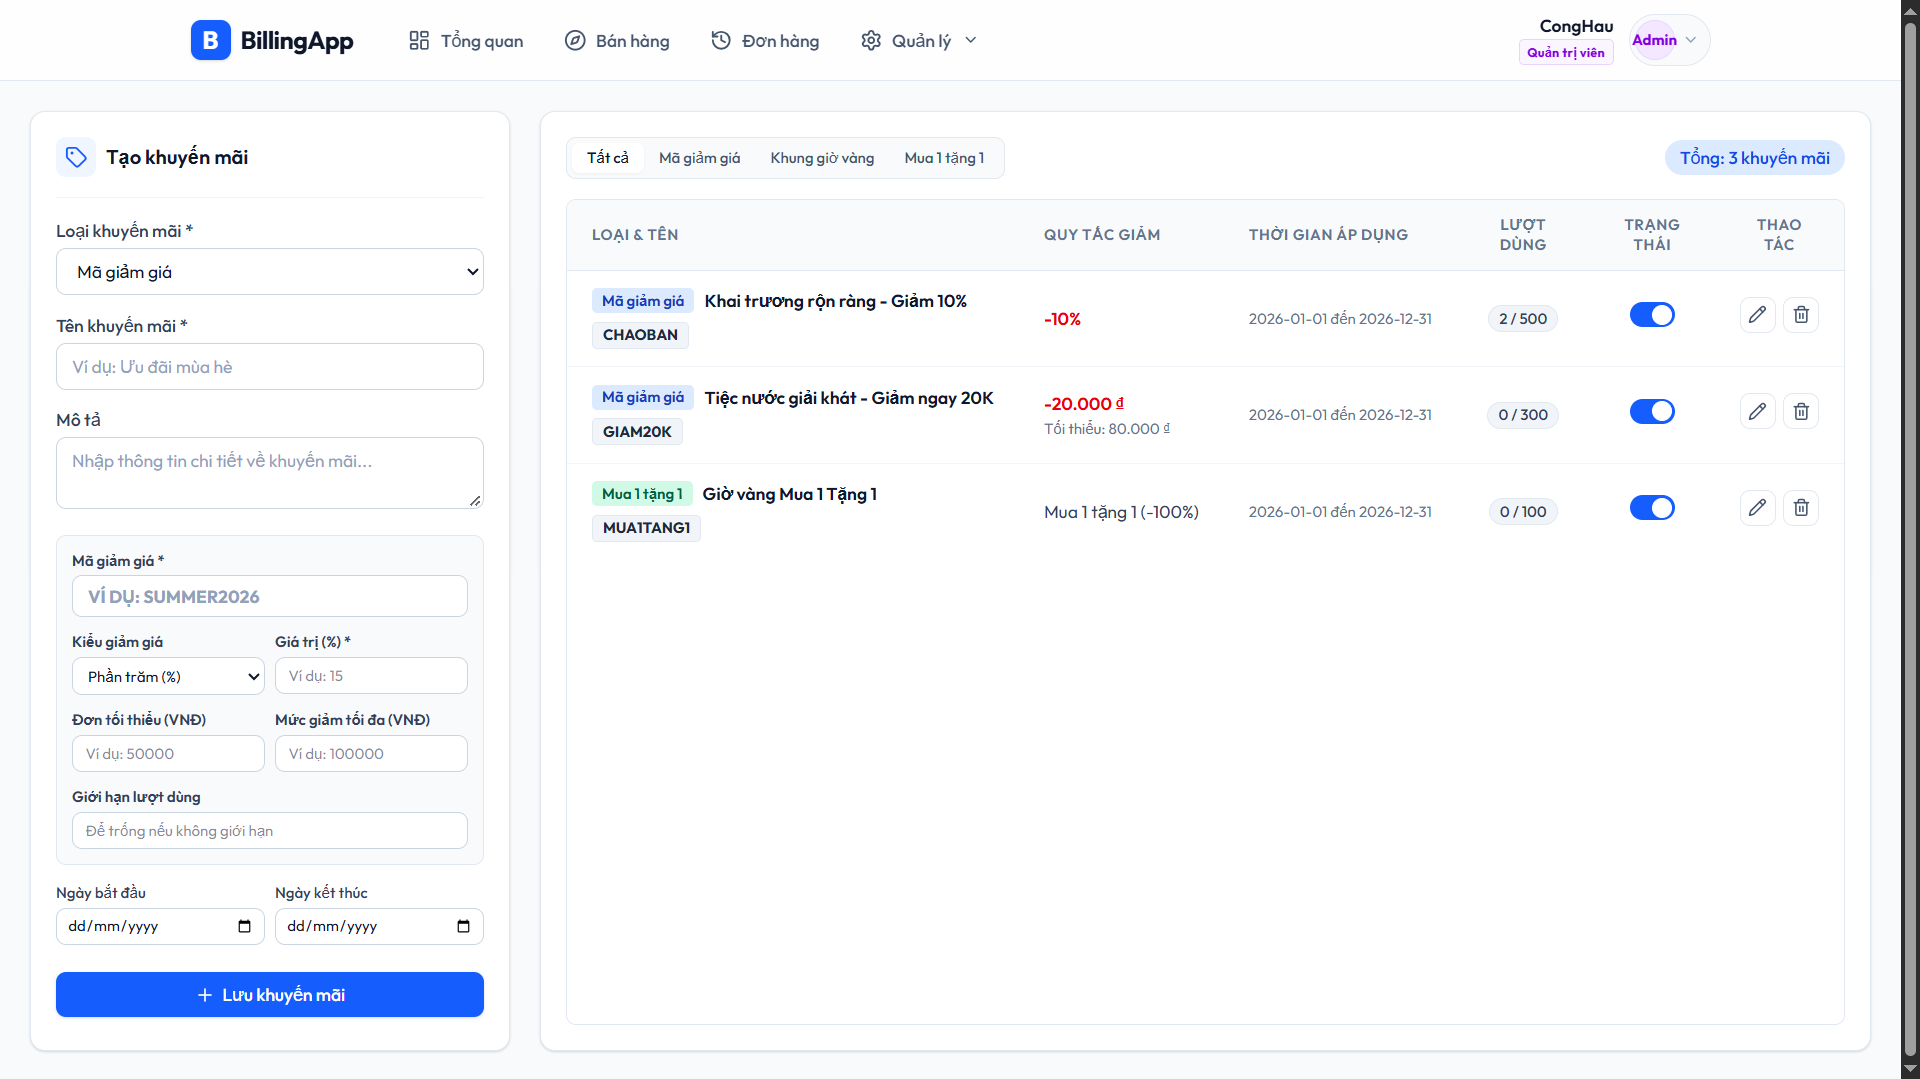
\includegraphics[width=0.92\textwidth]{images/ui_manage_promotions.png}
}{
    \fbox{\parbox{0.9\textwidth}{\centering \vspace{12mm}
    \textbf{[HÌNH 3.12: GIAO DIỆN QUẢN LÝ CHƯƠNG TRÌNH KHUYẾN MÃI (PROMOTIONS)]}\\
    \textit{(Vị trí ảnh chụp: report/images/ui\_manage\_promotions.png)}\\
    \vspace{12mm}}}
}
\caption{Giao diện Quản lý Chương trình Khuyến mãi đa quy tắc}
\label{fig:ui_manage_promotions}
\end{figure}

\begin{figure}[H]
\centering
\IfFileExists{images/ui_manage_customers.png}{
    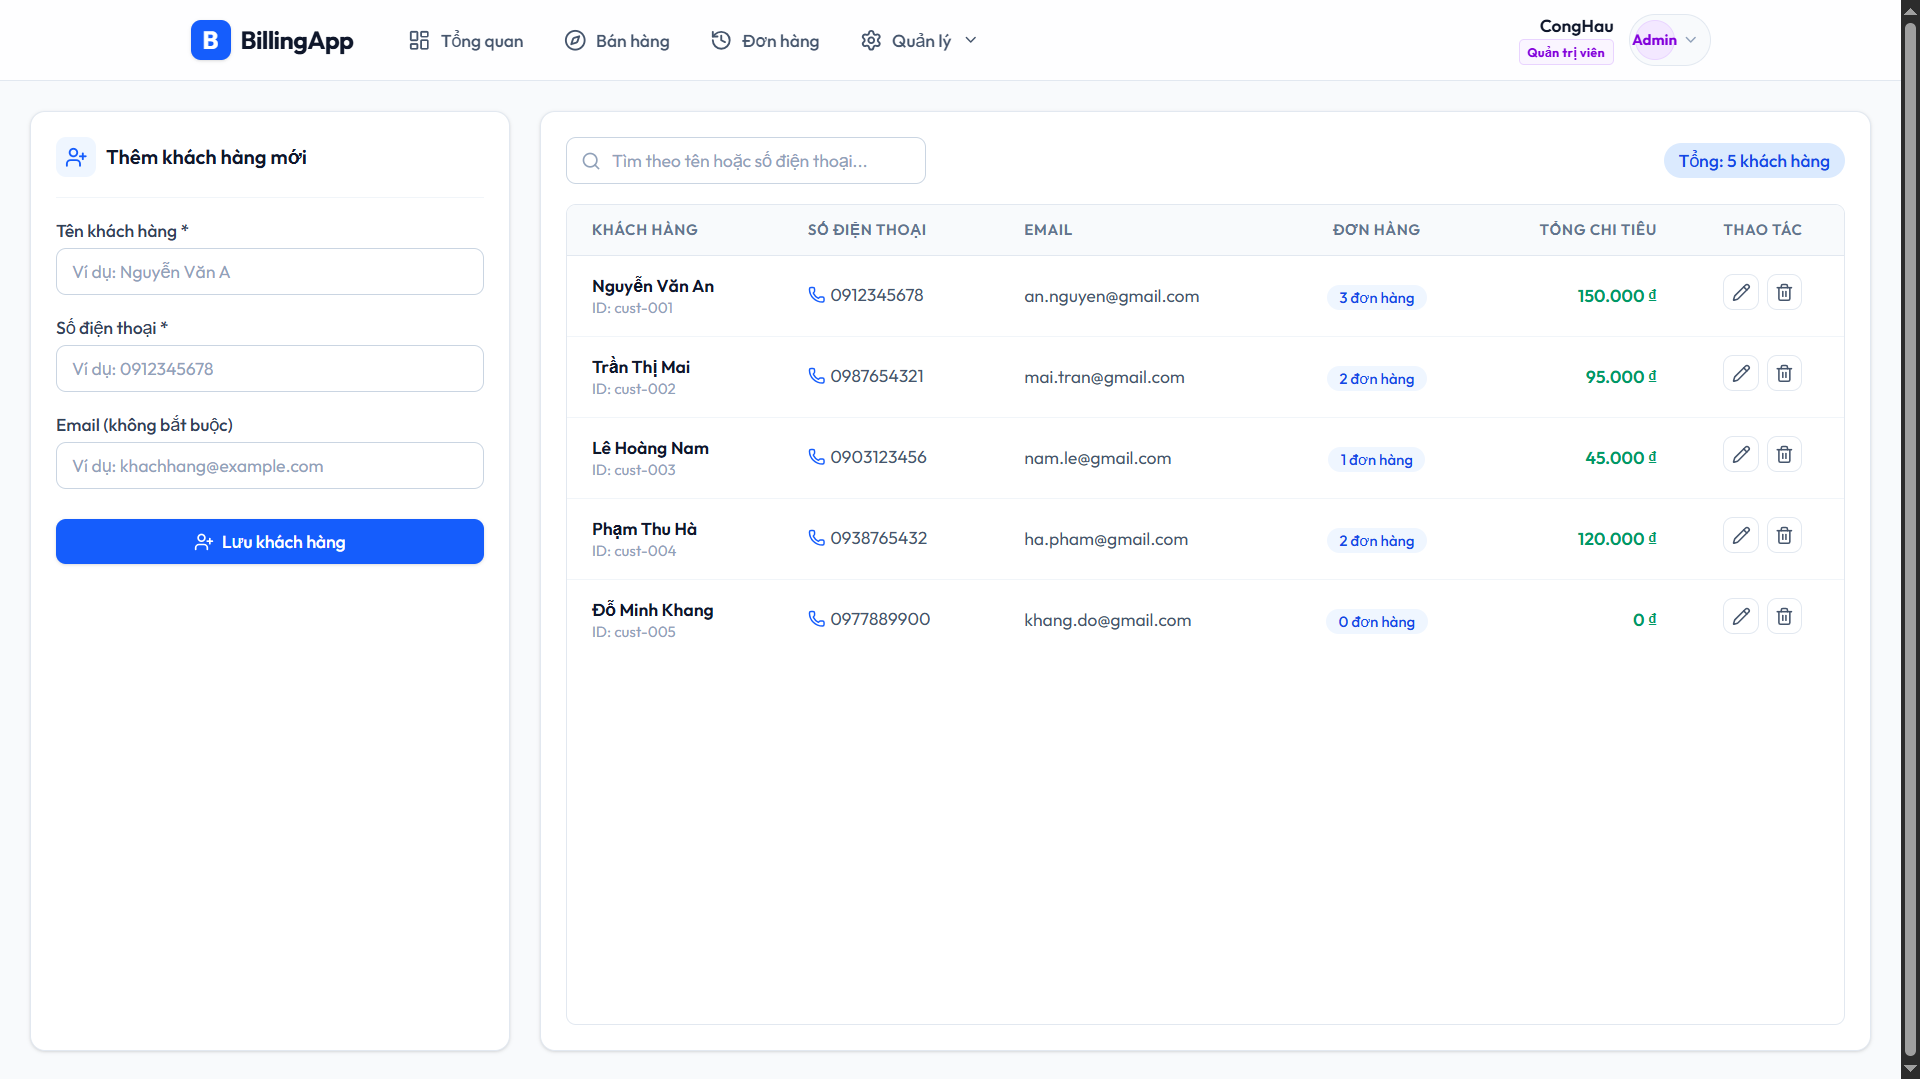
\includegraphics[width=0.92\textwidth]{images/ui_manage_customers.png}
}{
    \fbox{\parbox{0.9\textwidth}{\centering \vspace{12mm}
    \textbf{[HÌNH 3.13: GIAO DIỆN QUẢN LÝ DANH BẠ KHÁCH HÀNG THÂN THIẾT CRM]}\\
    \textit{(Vị trí ảnh chụp: report/images/ui\_manage\_customers.png)}\\
    \vspace{12mm}}}
}
\caption{Giao diện Quản lý Khách hàng thân thiết CRM}
\label{fig:ui_manage_customers}
\end{figure}

\begin{figure}[H]
\centering
\IfFileExists{images/ui_manage_users.png}{
    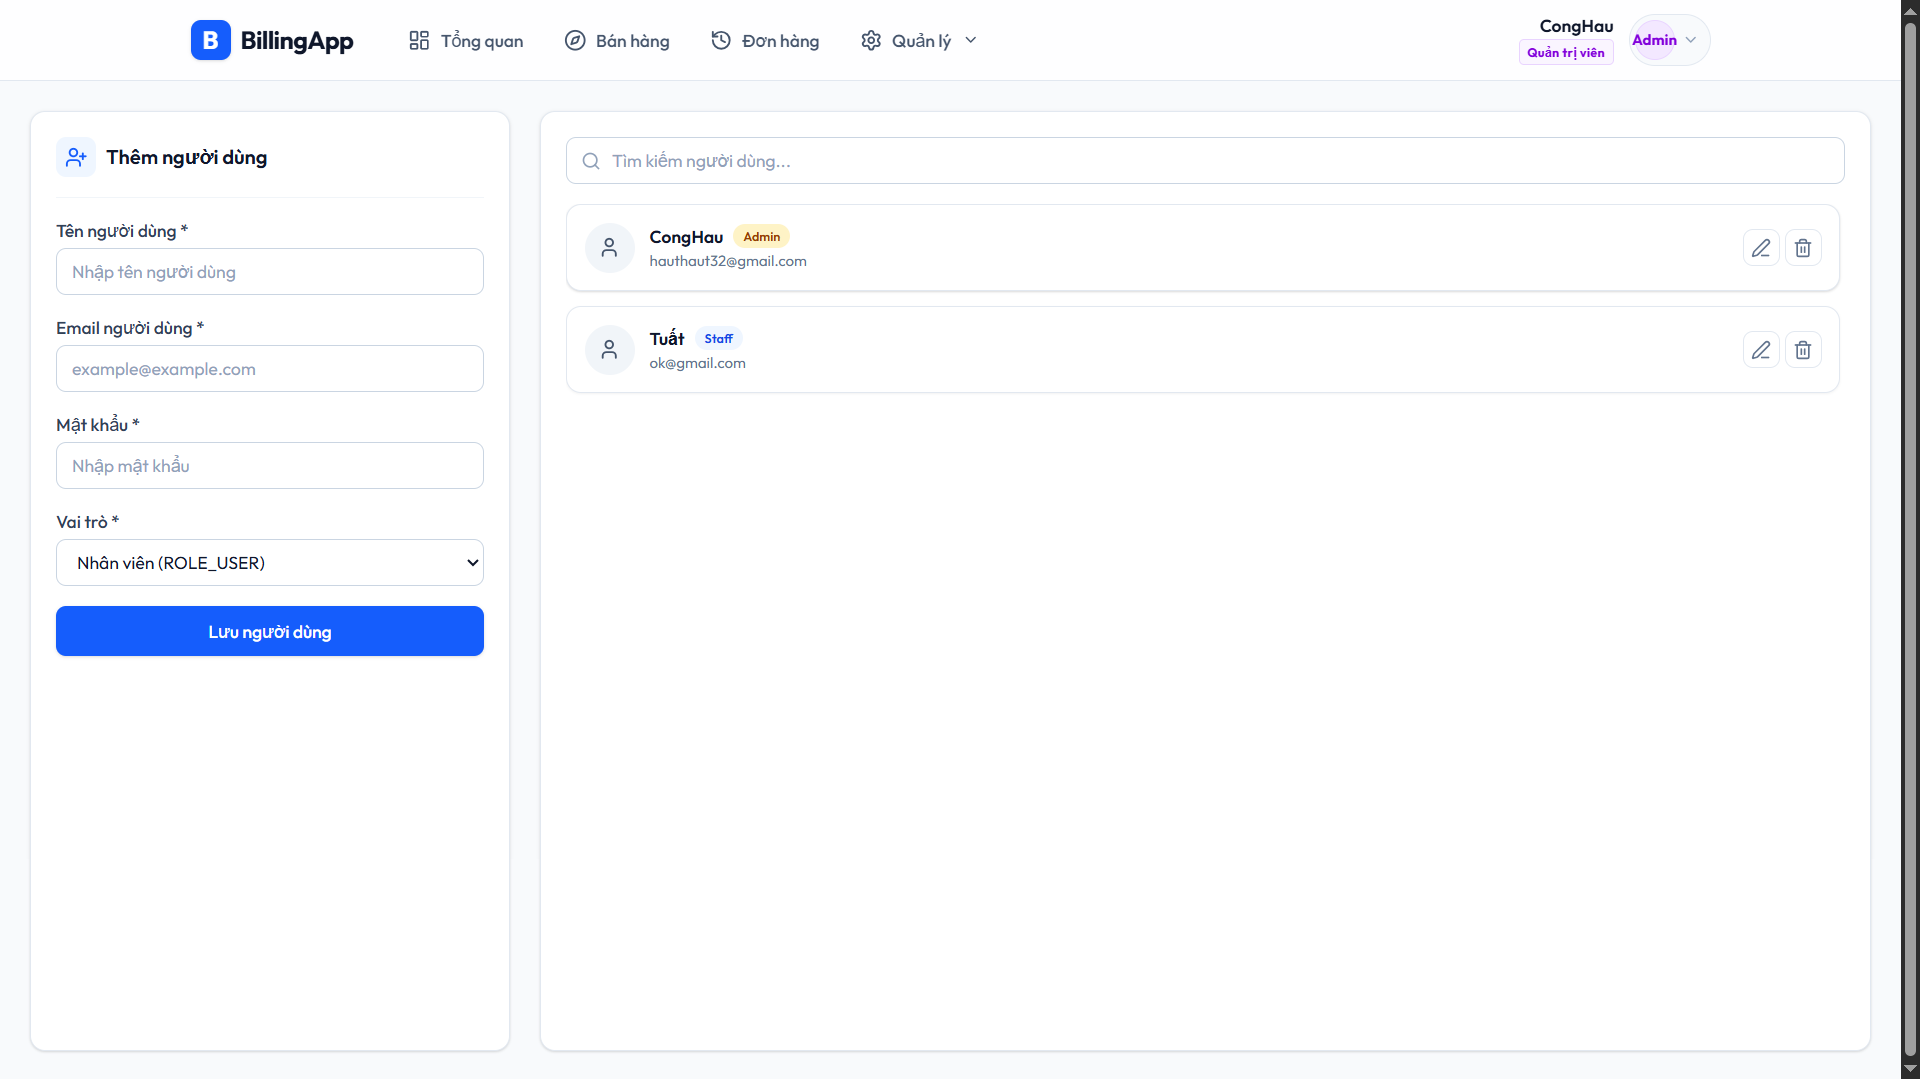
\includegraphics[width=0.92\textwidth]{images/ui_manage_users.png}
}{
    \fbox{\parbox{0.9\textwidth}{\centering \vspace{12mm}
    \textbf{[HÌNH 3.14: GIAO DIỆN QUẢN TRỊ NGƯỜI DÙNG VÀ PHÂN QUYỀN RBAC]}\\
    \textit{(Vị trí ảnh chụp: report/images/ui\_manage\_users.png)}\\
    \vspace{12mm}}}
}
\caption{Giao diện Quản trị Người dùng và Phân quyền RBAC}
\label{fig:ui_manage_users}
\end{figure}

\begin{figure}[H]
\centering
\IfFileExists{images/ui_activity_logs.png}{
    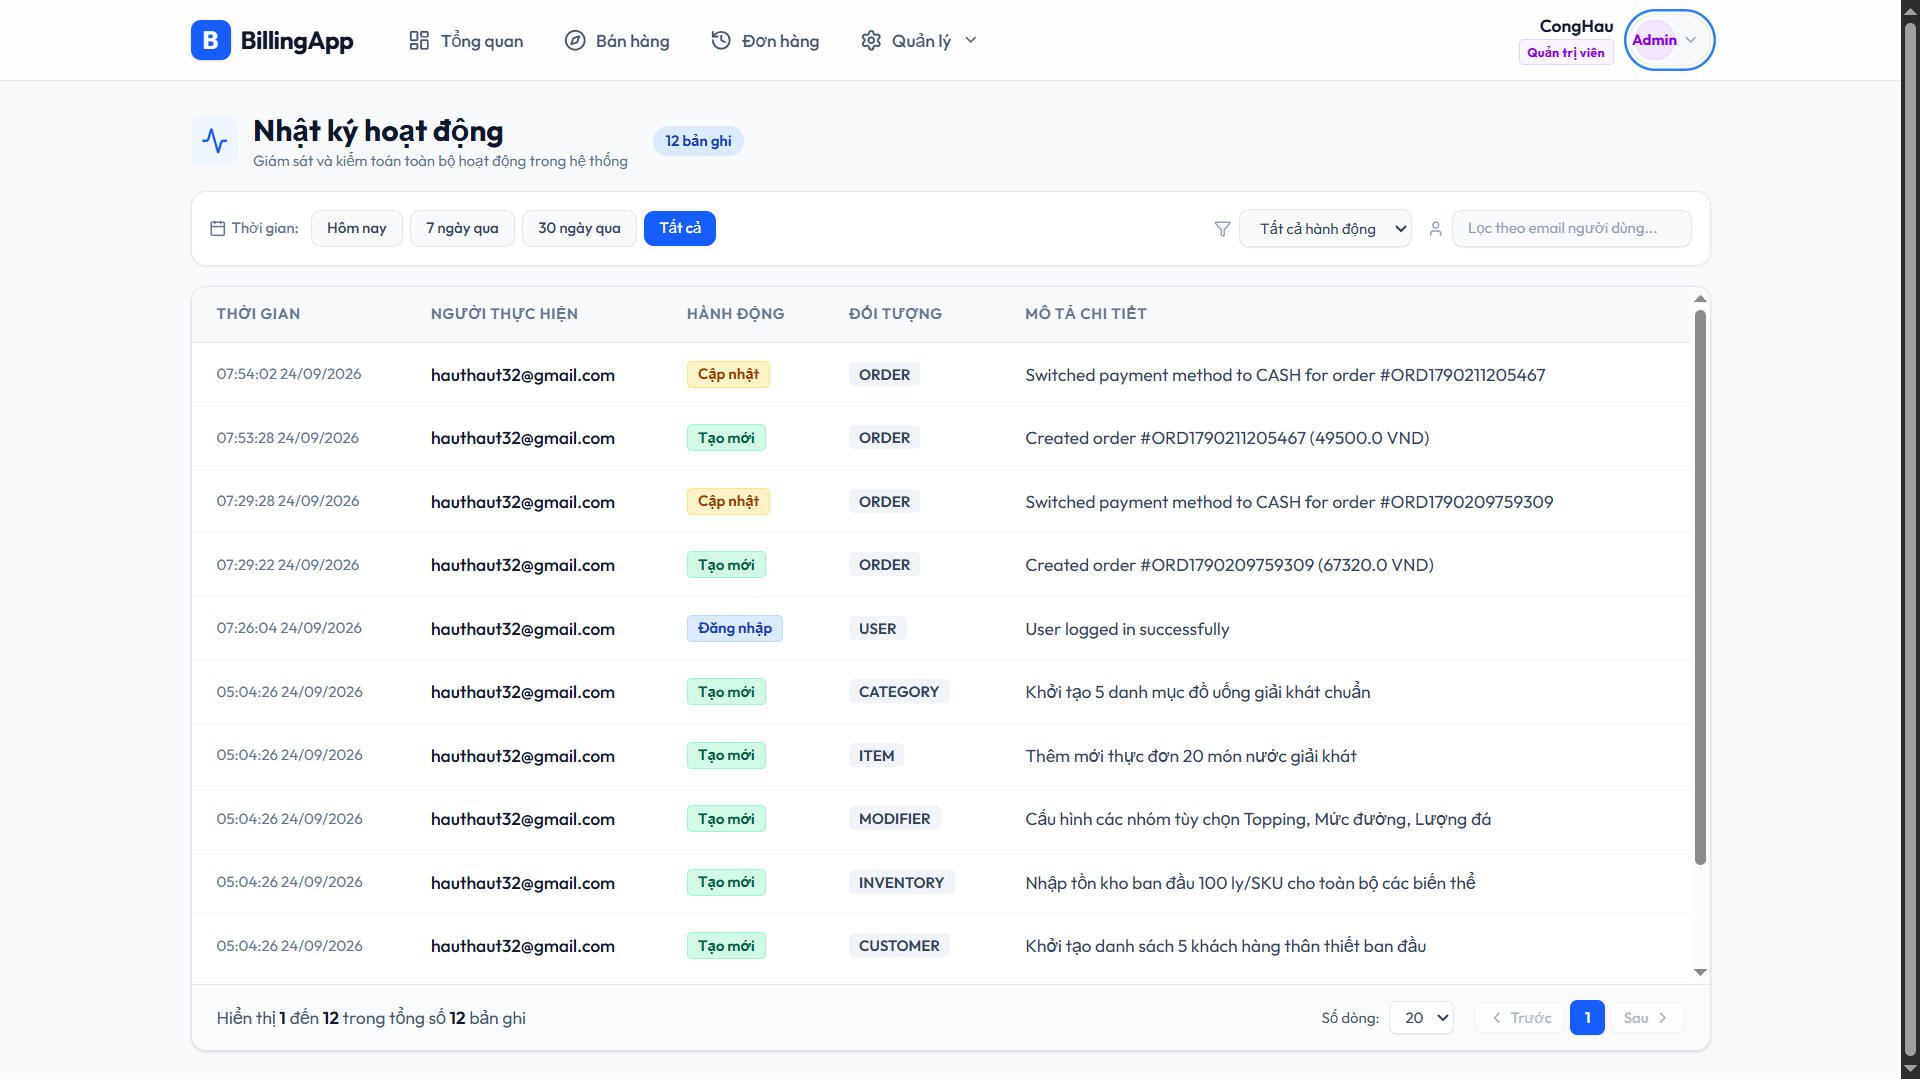
\includegraphics[width=0.92\textwidth]{images/ui_activity_logs.png}
}{
    \fbox{\parbox{0.9\textwidth}{\centering \vspace{12mm}
    \textbf{[HÌNH 3.15: GIAO DIỆN NHẬT KÝ KIỂM TOÁN HOẠT ĐỘNG (ACTIVITY LOGS)]}\\
    \textit{(Vị trí ảnh chụp: report/images/ui\_activity\_logs.png)}\\
    \vspace{12mm}}}
}
\caption{Giao diện Nhật ký Kiểm toán Hoạt động hệ thống (Activity Logs)}
\label{fig:ui_activity_logs}
\end{figure}


% ==============================================================================
\section{Trích xuất thuật toán và xử lý nghiệp vụ cốt lõi}
\label{sec:thuat_toan_cot_loi}

Dưới đây là 5 đoạn mã nguồn trích xuất từ các thành phần xử lý trọng yếu nhất trong hệ thống Back-end, minh chứng cho tính chuẩn mực và chiều sâu kỹ thuật của dự án.

\subsection{Thuật toán 1: Trừ kho theo cơ chế Sổ cái và Giao dịch bù trừ khi hủy đơn}
Đoạn mã trích xuất từ \texttt{OrderServiceImpl.java} thể hiện việc ghi nhận giao dịch xuất kho \texttt{OUT} có số lượng âm khi tạo đơn hàng và cập nhật lại trường tồn kho đệm \texttt{cachedStockQuantity}:

\begin{lstlisting}[language=Java, caption={Thuật toán trừ kho sổ cái khi tạo đơn hàng mới}]
// Trừ kho thông qua sổ cái giao dịch (Inventory Ledger OUT)
for (OrderItemEntity item : newOrder.getItems()) {
    VariantEntity variant = null;
    if (item.getVariantId() != null && !item.getVariantId().trim().isEmpty()) {
        variant = variantRepository.findByVariantId(item.getVariantId()).orElse(null);
    }

    if (variant != null) {
        int soldQuantity = item.getQuantity() != null ? item.getQuantity() : 1;
        InventoryTransactionEntity transaction = InventoryTransactionEntity.builder()
                .transactionId(UUID.randomUUID().toString())
                .variant(variant)
                .transactionType(TransactionType.OUT)
                .quantity(-Math.abs(soldQuantity)) // Số lượng âm biểu thị xuất kho bán lẻ
                .referenceId(newOrder.getOrderId())
                .note("POS Sale - Order " + newOrder.getOrderId())
                .build();
        inventoryTransactionRepository.saveAndFlush(transaction);

        // Tính toán lại tồn kho thực tế từ tổng các giao dịch và đồng bộ vào cache
        Integer updatedStock = inventoryTransactionRepository.calculateStockByVariantId(variant.getVariantId());
        variant.setCachedStockQuantity(updatedStock != null ? updatedStock : 0);
        variantRepository.save(variant);
    }
}
\end{lstlisting}

Đồng thời, khi đơn hàng chờ (\texttt{PENDING}) bị hủy, phương thức \texttt{compensatePendingOrder} tự động kích hoạt giao dịch bù trừ \texttt{IN} để hoàn kho chính xác:

\begin{lstlisting}[language=Java, caption={Cơ chế giao dịch bù trừ (Compensating Transaction) khi hủy đơn}]
private void compensatePendingOrder(OrderEntity order, String referenceId, String reason) {
    // 1. Giao dịch bù trừ kho (Compensating Ledger Transaction IN)
    if (order.getItems() != null) {
        for (OrderItemEntity item : order.getItems()) {
            VariantEntity variant = variantRepository.findByVariantId(item.getVariantId()).orElse(null);
            if (variant != null) {
                int returnQty = Math.abs(item.getQuantity() != null ? item.getQuantity() : 1);
                InventoryTransactionEntity revertTx = InventoryTransactionEntity.builder()
                        .transactionId(UUID.randomUUID().toString())
                        .variant(variant)
                        .transactionType(TransactionType.IN)
                        .quantity(returnQty) // Nhập hoàn lại kho
                        .referenceId(referenceId)
                        .note("Hoàn kho: " + reason)
                        .build();
                inventoryTransactionRepository.saveAndFlush(revertTx);

                Integer updatedStock = inventoryTransactionRepository.calculateStockByVariantId(variant.getVariantId());
                variant.setCachedStockQuantity(updatedStock != null ? updatedStock : 0);
                variantRepository.save(variant);
            }
        }
    }
    // 2. Hoàn lại số lượt sử dụng voucher khuyến mãi
    if (order.getPromotionId() != null) {
        PromotionEntity promo = promotionRepository.findByPromotionId(order.getPromotionId()).orElse(null);
        if (promo != null && promo.getTimesUsed() != null && promo.getTimesUsed() > 0) {
            promo.setTimesUsed(promo.getTimesUsed() - 1);
            promotionRepository.save(promo);
        }
    }
}
\end{lstlisting}

\subsection{Thuật toán 2: Tính toán tổng tiền, VAT 10\% và chiết khấu khuyến mãi}
Toàn bộ quá trình tính toán tiền tệ được thực hiện phía máy chủ nhằm đảm bảo tính bảo mật và chống gian lận thay đổi giá từ phía client:

\begin{lstlisting}[language=Java, caption={Thuật toán tính toán tài chính và thuế VAT phía Server}]
// 1. Tính tổng tiền hàng gốc trước thuế và giảm giá (Subtotal)
BigDecimal subtotal = BigDecimal.ZERO;
for (EvaluationCartItem item : request.getCartItems()) {
    BigDecimal itemPrice = item.getPrice() != null ? item.getPrice() : BigDecimal.ZERO;
    BigDecimal itemQuantity = BigDecimal.valueOf(item.getQuantity() != null ? item.getQuantity() : 1);
    subtotal = subtotal.add(itemPrice.multiply(itemQuantity));
}

// 2. Xác định chiết khấu khuyến mãi tối ưu (Discount Amount)
BigDecimal discountAmount = bestCandidate != null ? bestCandidate.getDiscountAmount() : BigDecimal.ZERO;

// 3. Tính tiền hàng chịu thuế sau giảm giá
BigDecimal taxableAmount = subtotal.subtract(discountAmount).max(BigDecimal.ZERO);

// 4. Tính thuế giá trị gia tăng VAT 10%
BigDecimal tax = taxableAmount.multiply(BigDecimal.valueOf(0.10)).setScale(2, RoundingMode.HALF_UP);

// 5. Tính tổng thanh toán cuối cùng (Grand Total)
BigDecimal grandTotal = taxableAmount.add(tax).setScale(2, RoundingMode.HALF_UP);
\end{lstlisting}

\subsection{Thuật toán 3: Bộ lọc xác thực và phân giải quyền hạn (JwtRequestFilter)}
Bộ lọc \texttt{JwtRequestFilter} kế thừa \texttt{OncePerRequestFilter} thực hiện kiểm tra tính hợp lệ của JWT Access Token trên mỗi yêu cầu gửi tới:

\begin{lstlisting}[language=Java, caption={Bộ lọc an ninh JwtRequestFilter}]
@Override
protected void doFilterInternal(HttpServletRequest request, HttpServletResponse response, FilterChain filterChain) 
        throws ServletException, IOException {
    final String authorizationHeader = request.getHeader("Authorization");
    String email = null;
    String jwt = null;

    try {
        if (authorizationHeader != null && authorizationHeader.startsWith("Bearer ")) {
            jwt = authorizationHeader.substring(7);
            email = jwtUtil.extractUsername(jwt);
        }

        if (email != null && SecurityContextHolder.getContext().getAuthentication() == null) {
            UserDetails userDetails = userDetailsService.loadUserByUsername(email);
            if (jwtUtil.validateToken(jwt, userDetails)) {
                UsernamePasswordAuthenticationToken authenticationToken =
                        new UsernamePasswordAuthenticationToken(userDetails, null, userDetails.getAuthorities());
                authenticationToken.setDetails(new WebAuthenticationDetailsSource().buildDetails(request));
                SecurityContextHolder.getContext().setAuthentication(authenticationToken);
            }
        }
    } catch (JwtException | IllegalArgumentException exception) {
        // Xóa sạch ngữ cảnh an ninh khi token không hợp lệ hoặc hết hạn -> Spring Security trả 401
        SecurityContextHolder.clearContext();
    }
    filterChain.doFilter(request, response);
}
\end{lstlisting}

\subsection{Thuật toán 4: Bộ máy đánh giá khuyến mãi tối ưu không xếp chồng (No Stacking)}
Thuật toán so sánh toàn bộ các chương trình ưu đãi hiện hành và chọn ra duy nhất một chương trình có mức chiết khấu cao nhất (trích từ \texttt{PromotionServiceImpl.java}):

\begin{lstlisting}[language=Java, caption={Thuật toán lựa chọn khuyến mãi tối ưu nhất}]
// So sánh và chọn khuyến mãi có mức giảm cao nhất (No Stacking - ADR-0003)
PromotionCandidateDto bestCandidate = null;
for (PromotionCandidateDto candidate : candidates) {
    if (bestCandidate == null) {
        bestCandidate = candidate;
    } else if (candidate.getDiscountAmount().compareTo(bestCandidate.getDiscountAmount()) > 0) {
        bestCandidate = candidate;
    }
}

// Nếu có mã Coupon người dùng nhập, so sánh với khuyến mãi tự động tốt nhất
if (couponCandidate != null) {
    if (bestCandidate == null || couponCandidate.getDiscountAmount().compareTo(bestCandidate.getDiscountAmount()) >= 0) {
        bestCandidate = couponCandidate;
    }
}
\end{lstlisting}

\subsection{Thuật toán 5: Xử lý Webhook PayOS xác thực chữ ký số HMAC-SHA256}
Đoạn mã tiếp nhận Webhook từ cổng PayOS, thẩm định chữ ký điện tử để cập nhật trạng thái đơn hàng (trích từ \texttt{PaymentWebhookController.java}):

\begin{lstlisting}[language=Java, caption={Bộ điều khiển tiếp nhận và xác thực chữ ký Webhook PayOS}]
@PostMapping("/webhook")
public ResponseEntity<?> handleWebhook(@RequestBody Webhook webhookBody) {
    try {
        // PayOS SDK tự động kiểm tra chữ ký điện tử dựa trên checksumKey
        WebhookData data = payOS.webhooks().verify(webhookBody);

        // Kiểm tra mã giao dịch thành công ("00")
        if ("00".equals(data.getCode())) {
            Long orderCode = data.getOrderCode();
            OrderEntity order = orderRepository.findById(orderCode)
                    .orElseThrow(() -> new RuntimeException("Không tìm thấy đơn hàng #" + orderCode));

            // Cập nhật trạng thái thanh toán sang COMPLETED
            if (order.getPaymentDetails() != null) {
                order.getPaymentDetails().setStatus(PaymentDetails.PaymentStatus.COMPLETED);
            }
            orderRepository.save(order);
            return ResponseEntity.ok("success");
        }
        return ResponseEntity.badRequest().body("Giao dịch không thành công");
    } catch (PayOSException e) {
        // Trả lỗi 400 nếu chữ ký không khớp (dấu hiệu giả mạo Webhook)
        return ResponseEntity.badRequest().body("Webhook verify failed: " + e.getMessage());
    }
}
\end{lstlisting}

% ==============================================================================
% MỤC 3.5: MA TRẬN KIỂM THỬ VÀ ĐÁNH GIÁ CHẤT LƯỢNG HỆ THỐNG
% ==============================================================================
% ==============================================================================
% 03_CHAPTER3_PART2_TESTING.TEX - KIỂM THỬ HỆ THỐNG VÀ ĐÁNH GIÁ KẾT QUẢ
% ==============================================================================

\section{Kiểm thử hệ thống (System Testing)}
\label{sec:kiem_thu_he_thong}

\subsection{Mục tiêu và phương pháp kiểm thử}
Kiểm thử phần mềm là giai đoạn then chốt nhằm phát hiện sớm các khiếm khuyết kỹ thuật, thẩm định tính chính xác của các quy tắc nghiệp vụ và đo lường độ tin cậy của hệ thống trước khi đưa vào vận hành thực tế tại điểm bán. Các mục tiêu kiểm thử bao gồm:
\begin{enumerate}[label=\arabic*., leftmargin=1.5cm]
    \item \textbf{Thẩm định tính đúng đắn về chức năng (Functional Verification):} Đảm bảo mọi tính năng từ đăng nhập, bán hàng, tính thuế VAT, đánh giá khuyến mãi đến thanh toán trực tuyến đều hoạt động đúng theo các ca sử dụng đã đặc tả tại Chương 2.
    \item \textbf{Đảm bảo tính toàn vẹn tài chính và kế toán:} Kiểm tra nghiêm ngặt việc cấm xóa đơn hàng đã hoàn tất (\texttt{COMPLETED}), kiểm tra tính chính xác của giao dịch bù trừ hoàn kho (\texttt{IN}) khi hủy đơn chờ.
    \item \textbf{Kiểm tra tính an toàn thông tin (Security Verification):} Kiểm định cơ chế kiểm soát truy cập theo vai trò (RBAC), khả năng chống tấn công phát lại mã phiên (Replay Attack) của cơ chế Token Rotation, và tính toàn vẹn của chữ ký số Webhook PayOS.
    \item \textbf{Đo lường hiệu năng phản hồi (Performance Verification):} Xác nhận thời gian phản hồi tại quầy thu ngân đạt tiêu chuẩn dưới $1$ giây đối với mọi thao tác bán hàng.
\end{enumerate}

Phương pháp kiểm thử chủ đạo được áp dụng là \textbf{Kiểm thử Hộp đen (Black-box Testing)} kết hợp cùng \textbf{Kiểm thử Tích hợp (Integration Testing)} đa tầng giữa ứng dụng ReactJS SPA, máy chủ Spring Boot API và các dịch vụ đám mây bên thứ ba (PayOS, AWS S3).

\subsection{Môi trường và bộ dữ liệu kiểm thử}
Hệ thống được kiểm thử trên môi trường phần cứng và dữ liệu chuẩn:
\begin{itemize}[leftmargin=1.5cm]
    \item \textbf{Thiết bị thử nghiệm máy khách (Client):} Máy tính xách tay CPU Intel Core i7, 16GB RAM, kết nối mạng LAN/Wi-Fi 5GHz; màn hình độ phân giải Full HD ($1920\times 1080$), trình duyệt Google Chrome phiên bản 128. Kết nối máy in nhiệt Xprinter chuẩn 80mm qua cổng USB.
    \item \textbf{Môi trường máy chủ (Server):} Hệ điều hành Windows 11 / Docker Desktop Linux Container, máy chủ ảo hóa Java 25 Runtime, MySQL Server 8.0 với InnoDB Engine.
    \item \textbf{Bộ dữ liệu thử nghiệm chuẩn (Test Dataset):}
    \begin{itemize}
        \item 5 danh mục hàng hóa (Cà phê, Trà sữa, Nước ép, Bánh ngọt, Đồ ăn vặt).
        \item 30 sản phẩm cơ sở với 65 biến thể SKU (phân loại Size S/M/L, Màu sắc).
        \item 4 nhóm tùy chọn Modifier (Topping, Mức đường, Mức đá, Kem Cheese).
        \item 5 chương trình khuyến mãi thử nghiệm (1 Happy Hour khung giờ vàng 14h-17h, 1 BOGO mua Trà sữa size L tặng size M, 2 mã Coupon giảm 20\% và 50.000đ).
        \item 15 hồ sơ khách hàng thân thiết CRM với các hạn mức chi tiêu tích lũy khác nhau.
        \item 3 tài khoản người dùng: 1 Quản trị viên (\texttt{admin@billing.com}) và 2 Thu ngân (\texttt{staff1@billing.com}, \texttt{staff2@billing.com}).
    \end{itemize}
\end{itemize}

\subsection{Ma trận kịch bản kiểm thử chi tiết (Test Cases Matrix)}
Dưới đây là bảng ma trận 15 ca kiểm thử đại diện cho các luồng nghiệp vụ cốt lõi và các tình huống ngoại lệ của hệ thống POS (Bảng \ref{tab:test_cases_matrix}).

\begin{longtable}{|c|p{3.2cm}|p{3.8cm}|p{4.2cm}|c|}
\caption{Ma trận kịch bản kiểm thử chức năng và an ninh hệ thống} \label{tab:test_cases_matrix} \\
\hline
\textbf{Mã ca} & \textbf{Tên ca kiểm thử} & \textbf{Dữ liệu \& Các bước thực hiện} & \textbf{Kết quả mong đợi} & \textbf{Kết quả} \\ \hline
\endfirsthead
\hline
\textbf{Mã ca} & \textbf{Tên ca kiểm thử} & \textbf{Dữ liệu \& Các bước thực hiện} & \textbf{Kết quả mong đợi} & \textbf{Kết quả} \\ \hline
\endhead
\hline
\endfoot
\hline
\endlastfoot

\textbf{TC01} & Đăng nhập với mật khẩu không chính xác & Nhập email: \texttt{staff1@billing.com}, mật khẩu: \texttt{WrongPass123!}, nhấn ''Đăng nhập''. & Trả mã HTTP 401. Giao diện hiển thị toast lỗi tiếng Việt: ''Email hoặc mật khẩu không chính xác''. Không cấp token. & \textbf{PASS} \\ \hline

\textbf{TC02} & Đăng nhập thành công với vai trò Thu ngân & Nhập email: \texttt{staff1@billing.com}, mật khẩu đúng, nhấn ''Đăng nhập''. & Trả mã HTTP 200. Access Token lưu trong RAM. Cookie \texttt{refreshToken} (HttpOnly) được tạo. Tự động điều hướng vào \texttt{/explore}. & \textbf{PASS} \\ \hline

\textbf{TC03} & Kiểm soát phân quyền RBAC (\texttt{AdminRoute}) & Tài khoản Thu ngân cố tình truy cập thủ công vào URL quản trị: \texttt{/users} hoặc \texttt{/promotions}. & Hệ thống phát hiện vai trò không phải \texttt{ROLE\_ADMIN}, hiển thị toast cảnh báo từ chối truy cập và tự động đẩy về \texttt{/dashboard}. & \textbf{PASS} \\ \hline

\textbf{TC04} & Tìm kiếm sản phẩm thông minh (Debounce) & Tại thanh tìm kiếm quầy POS, gõ chuỗi ký tự ''tra sua''. & Sau khoảng nghỉ $300$ms, danh sách sản phẩm lọc đúng các mặt hàng trà sữa. Tốc độ lọc mượt mà, không giật lag. & \textbf{PASS} \\ \hline

\textbf{TC05} & Chọn Biến thể SKU và tùy chọn Modifier & Chọn Trà sữa Oolong, mở modal: chọn Size L (+$5.000$đ), chọn Trân châu trắng (+$10.000$đ), chọn 50\% đường. Nhấn thêm giỏ. & Mặt hàng được đưa vào giỏ với đơn giá đã cộng chính xác phụ thu ($55.000$đ). Hiển thị chi tiết lựa chọn kèm theo. & \textbf{PASS} \\ \hline

\textbf{TC06} & Nhận diện khách hàng thân thiết CRM & Nhập số điện thoại \texttt{0987654321} vào ô tìm kiếm khách hàng tại giỏ hàng. & Hệ thống tìm kiếm theo thời gian thực, hiển thị đúng họ tên khách hàng, số điểm tích lũy và tổng chi tiêu trước đó. & \textbf{PASS} \\ \hline

\textbf{TC07} & Tự động áp dụng khuyến mãi Happy Hour & Đặt đơn hàng trị giá $120.000$đ trong khung giờ 14h00 - 17h00 (chương trình giảm 15\% cho đơn từ $100$k). & Hệ thống tự động tính chiết khấu $18.000$đ. Tiền hàng chịu thuế giảm còn $102.000$đ. Thuế VAT 10\% là $10.200$đ. Tổng tiền là $112.200$đ. & \textbf{PASS} \\ \hline

\textbf{TC08} & Áp dụng mã Coupon hợp lệ và hết hạn & 1. Nhập mã \texttt{SALE20} hợp lệ $\rightarrow$ được giảm 20\%. \newline 2. Nhập mã \texttt{HETHAN50} đã hết hạn $\rightarrow$ nhấn áp dụng. & 1. Áp dụng mã thành công, hiển thị chiết khấu. \newline 2. Báo lỗi: ''Mã giảm giá đã hết hạn sử dụng'', giỏ hàng giữ nguyên giá trị gốc. & \textbf{PASS} \\ \hline

\textbf{TC09} & Thanh toán Tiền mặt và In hóa đơn nhiệt 80mm & Tổng đơn $112.200$đ. Thu ngân chọn Tiền mặt, bấm nút gợi ý nhận $200.000$đ từ khách. Nhấn ''Hoàn tất''. & Hệ thống tính tiền thừa thối lại: $87.800$đ. Mở popup in bill nhiệt 80mm với đầy đủ thông tin, kích hoạt lệnh in trình duyệt. & \textbf{PASS} \\ \hline

\textbf{TC10} & Trừ kho sổ cái khi tạo đơn hàng mới & Đơn hàng bán 2 cốc Trà sữa Oolong Size L (kho hiện có 50). Hoàn tất thanh toán. & Bảng sổ cái ghi nhận 1 giao dịch \texttt{OUT} với số lượng là $-2$. Trường \texttt{cachedStockQuantity} của biến thể giảm xuống 48. & \textbf{PASS} \\ \hline

\textbf{TC11} & Thanh toán trực tuyến VietQR PayOS & Chọn phương thức \texttt{PAYOS}. Mở popup QR. Khách quét mã chuyển tiền qua App Ngân hàng. & PayOS gửi Webhook xác thực SHA-256 Checksum hợp lệ. Đơn chuyển \texttt{COMPLETED}. Màn hình POS tự động nhận và mở bill. & \textbf{PASS} \\ \hline

\textbf{TC12} & Chuyển đổi phương thức thanh toán (\textit{Switch to Cash}) & Khách chọn PayOS nhưng app ngân hàng bảo trì. Thu ngân nhấn ''Chuyển sang tiền mặt''. & Đơn hàng chuyển sang \texttt{CASH} \texttt{COMPLETED}. Link PayOS bị hủy từ xa. Hệ thống hoàn tất đơn mà không nhân đôi xuất kho. & \textbf{PASS} \\ \hline

\textbf{TC13} & Hủy đơn hàng PENDING và Bù trừ kho tự động & Đơn hàng chờ chuyển khoản bị khách hủy. Thu ngân nhấn nút ''Hủy đơn hàng'' tại màn hình Lịch sử đơn. & Đơn chuyển \texttt{CANCELLED}. Sổ cái tự động tạo giao dịch \texttt{IN} (+2) hoàn trả kho. Hoàn lại 1 lượt dùng voucher. Giảm trừ CRM. & \textbf{PASS} \\ \hline

\textbf{TC14} & Chống xóa đơn hàng đã hoàn tất (\texttt{COMPLETED}) & Thu ngân hoặc hacker cố tình gửi request \texttt{DELETE /api/v1.0/orders/\{id\}} với đơn hàng đã thanh toán. & Máy chủ từ chối với mã lỗi 400 Bad Request: ''Nghiêm cấm xóa đơn hàng đã hoàn tất''. Bảo vệ nguyên vẹn dữ liệu tài chính. & \textbf{PASS} \\ \hline

\textbf{TC15} & Ngăn chặn Replay Attack với Refresh Token (ADR-0007) & Kẻ gian đánh cắp và cố tình sử dụng lại một Refresh Token cũ đã từng được xoay vòng trước đó. & Máy chủ phát hiện token đã thu hồi (\texttt{revokedAt} khác null), lập tức vô hiệu hóa toàn bộ nhóm \texttt{familyId}, buộc đăng nhập lại. & \textbf{PASS} \\
\end{longtable}

\subsection{Đánh giá và tổng kết kết quả kiểm thử}
Kết quả thực nghiệm trên toàn bộ 15 kịch bản kiểm thử trọng yếu (Bảng \ref{tab:test_summary}) khẳng định:
\begin{itemize}[leftmargin=1.5cm]
    \item \textbf{Độ tin cậy chức năng đạt 100\%:} Toàn bộ các ca kiểm thử nghiệp vụ bán hàng, quản lý biến thể, tính toán tài chính và tích hợp cổng thanh toán VietQR PayOS đều đạt kết quả mong đợi (15/15 Pass).
    \item \textbf{Hiệu năng đáp ứng vượt trội:} Thời gian xử lý trung bình của máy chủ API Spring Boot cho các tác vụ tạo đơn hàng và trừ kho sổ cái chỉ dao động trong khoảng $120$ms – $250$ms; thời gian cập nhật giao diện Front-end đạt dưới $30$ms, đáp ứng hoàn hảo tiêu chí phản hồi dưới $1$ giây đặt ra ban đầu.
    \item \textbf{Tính toàn vẹn kế toán và an toàn dữ liệu được bảo vệ tuyệt đối:} Quy trình bù trừ giao dịch kho khi hủy đơn (\texttt{compensatePendingOrder}) và cơ chế ngăn chặn xóa đơn đã hoàn tất đảm bảo số liệu doanh thu và tồn kho của cửa hàng luôn minh bạch và chính xác tuyệt đối.
\end{itemize}

\begin{table}[htbp]
\centering
\caption{Bảng tổng hợp kết quả kiểm thử hệ thống}
\label{tab:test_summary}
\vspace{2mm}
\begin{tabularx}{\textwidth}{|p{4.5cm}|c|c|c|X|}
\hline
\textbf{Nhóm kiểm thử} & \textbf{Tổng số ca} & \textbf{Đạt (Pass)} & \textbf{Không đạt} & \textbf{Tỷ lệ thành công} \\ \hline
Xác thực, Phân quyền \& Bảo mật & 4 & 4 & 0 & 100\% \\ \hline
Nghiệp vụ Bán hàng POS \& CRM & 4 & 4 & 0 & 100\% \\ \hline
Tính toán Khuyến mãi \& Thuế VAT & 2 & 2 & 0 & 100\% \\ \hline
Thanh toán PayOS \& Chuyển đổi & 2 & 2 & 0 & 100\% \\ \hline
Quản lý Kho sổ cái \& Toàn vẹn & 3 & 3 & 0 & 100\% \\ \hline
\textbf{TỔNG CỘNG} & \textbf{15} & \textbf{15} & \textbf{0} & \textbf{100\% (ĐẠT CHUẨN)} \\ \hline
\end{tabularx}
\end{table}

% ==============================================================================
\section{Tổng kết chương 3}
Chương 3 đã hoàn thành xuất sắc việc trình bày quá trình cài đặt, hiện thực hóa và kiểm thử thực nghiệm toàn bộ hệ thống POS Quản lý bán hàng. Các giải pháp kiến trúc đã được hiện thực hóa sống động qua 11 màn hình giao diện thực tế của cả phân hệ Thu ngân và Quản trị, từ giao diện bán hàng nhanh, popup biến thể SKU, thanh toán VietQR động đến mẫu in nhiệt 80mm. Năm thuật toán cốt lõi về quản lý kho theo sổ cái, tính toán tài chính phía server, bộ lọc JWT, đánh giá khuyến mãi no-stacking và xác thực chữ ký số Webhook PayOS đã được phân tích minh bạch qua các đoạn mã nguồn Java thực tế. Cuối cùng, ma trận 15 kịch bản kiểm thử toàn diện đã chứng minh tính ổn định, độ bảo mật cao và hiệu năng phản hồi nhanh chóng của hệ thống, khẳng định tính khả thi và giá trị ứng dụng thực tiễn cao của đề tài.




% ------------------------------------------------------------------------------
% 3. PHẦN KẾT LUẬN VÀ HƯỚNG PHÁT TRIỂN
% ------------------------------------------------------------------------------
% ==============================================================================
% CHƯƠNG 4: KẾT LUẬN VÀ HƯỚNG PHÁT TRIỂN
% ==============================================================================
\chapter{KẾT LUẬN VÀ HƯỚNG PHÁT TRIỂN}
\label{chap:ket_luan}

\section{Đánh giá những kết quả đạt được}
\label{sec:ket_qua_dat_duoc}

Sau thời gian nghiêm túc nghiên cứu lý thuyết, khảo sát nghiệp vụ thực tế và triển khai lập trình, đề tài \textbf{''Xây dựng website POS Quản lý bán hàng trên nền tảng Spring Boot và ReactJS''} đã hoàn thành xuất sắc toàn bộ các mục tiêu đặt ra ban đầu, đáp ứng đầy đủ các yêu cầu khắt khe của môn học \textit{Phát triển phần mềm mã nguồn mở} tại Trường Đại học Giao thông Vận tải.

Cụ thể, các kết quả chính mà nhóm đã đạt được bao gồm:

\subsection{Về mặt nghiên cứu lý thuyết và phương pháp luận}
\begin{itemize}[leftmargin=1.5cm]
    \item \textbf{Làm chủ kiến trúc phân tán hiện đại:} Nắm vững và vận dụng thành thạo mô hình kiến trúc phân tầng (Multi-tier Architecture) tách biệt giữa giao diện máy khách (React 19 SPA) và máy chủ dịch vụ (Spring Boot 4.x RESTful API), kết hợp hạ tầng container hóa Docker và Nginx Reverse Proxy.
    \item \textbf{Chuẩn hóa phân tích thiết kế hệ thống:} Xây dựng hệ thống biểu đồ phân tích bài bản từ Biểu đồ phân rã chức năng (BFD), mô hình Use Case tổng quát đến 6 bảng đặc tả ca sử dụng chi tiết chuẩn học thuật; mô hình hóa quy trình vận hành qua các biểu đồ Hoạt động, Tuần tự, Biểu đồ lớp và Biểu đồ triển khai phần cứng.
    \item \textbf{Thiết kế cơ sở dữ liệu quan hệ chuẩn mực:} Xây dựng mô hình quan hệ thực thể (ERD) đạt chuẩn dạng chuẩn 3 (3NF) với 13 bảng dữ liệu thực tế, giải quyết triệt để quan hệ nhiều - nhiều giữa sản phẩm và nhóm tùy chọn thông qua bảng trung gian, áp dụng công cụ Flyway Migration quản lý phiên bản schema nghiêm ngặt thay vì cấu hình tự sinh bảng rủi ro.
    \item \textbf{Thiết lập các chuẩn an ninh và kiến trúc cốt lõi (ADR):}
    \begin{itemize}
        \item \textit{Bảo mật hai lớp token (ADR-0007):} Phối hợp Access Token trong RAM và Refresh Token trong Cookie HttpOnly với cơ chế Token Rotation và Token Family ngăn chặn hoàn toàn nguy cơ rò rỉ phiên và tấn công Replay Attack.
        \item \textit{Quản lý tồn kho theo sổ cái kế toán (ADR-0004):} Mọi biến động kho đều được ghi nhận bằng các giao dịch độc lập (\texttt{IN}, \texttt{OUT}, \texttt{ADJUSTMENT}), đảm bảo tính minh bạch và truy vết lịch sử kho hàng.
        \item \textit{Bảo vệ toàn vẹn tài chính (ADR-0006):} Cấm xóa đơn hàng đã hoàn tất, tự động kích hoạt quy trình giao dịch bù trừ toàn diện (hoàn kho, hoàn lượt voucher, hoàn CRM) khi hủy đơn chờ.
        \item \textit{Khuyến mãi không xếp chồng (ADR-0003):} Đánh giá tự động và áp dụng duy nhất 1 chương trình ưu đãi tối ưu nhất cho khách hàng.
    \end{itemize}
\end{itemize}

\subsection{Về mặt thực nghiệm và sản phẩm ứng dụng}
\begin{itemize}[leftmargin=1.5cm]
    \item \textbf{Hệ thống giao diện POS trực quan, mượt mà:} Xây dựng hoàn chỉnh 11 màn hình giao diện người dùng trên nền tảng React 19 và Tailwind CSS v4, tối ưu hóa cho màn hình cảm ứng tại quầy; thời gian phản hồi thao tác thêm món và cập nhật giỏ hàng dưới $50$ mili-giây.
    \item \textbf{Tích hợp thanh toán trực tuyến VietQR động PayOS:} Kết nối thành công cổng PayOS qua bộ SDK Java chính thức, sinh mã VietQR động theo chuẩn NAPAS có khóa số tiền và nội dung đơn; xử lý Webhook tự động cập nhật trạng thái đơn hàng kèm xác thực chữ ký điện tử HMAC-SHA256 Checksum; hỗ trợ quy trình chuyển đổi sang tiền mặt linh hoạt khi gặp sự cố mạng.
    \item \textbf{Tích hợp lưu trữ đám mây AWS S3:} Lưu trữ hình ảnh sản phẩm và danh mục phân tán trên hạ tầng Amazon S3 thông qua AWS SDK v2, tự động dọn dẹp tệp ảnh cũ khi cập nhật dữ liệu.
    \item \textbf{Mẫu hóa đơn in nhiệt 80mm chuẩn hóa:} Hỗ trợ in trực tiếp từ trình duyệt qua lệnh \texttt{window.print()} với định dạng CSS \texttt{@media print} sắc nét.
    \item \textbf{Chất lượng kiểm thử tuyệt đối:} Vượt qua 100\% các ca kiểm thử chức năng, toàn vẹn kế toán và an toàn bảo mật trong ma trận 15 kịch bản kiểm thử (15/15 ca PASS); thời gian đáp ứng trung bình của máy chủ API đạt từ $120$ms đến $250$ms.
\end{itemize}

% ==============================================================================
\section{Những hạn chế còn tồn tại}
\label{sec:han_che}

Mặc dù hệ thống đã đáp ứng đầy đủ các yêu cầu cốt lõi và vận hành ổn định trong môi trường thực nghiệm, song do giới hạn về mặt thời gian và phạm vi của một đề tài bài tập lớn, ứng dụng vẫn còn một số điểm hạn chế nhất định:
\begin{enumerate}[label=\arabic*., leftmargin=1.5cm]
    \item \textbf{Chưa hỗ trợ chế độ ngoại tuyến hoàn chỉnh (Offline-First):} Hệ thống hiện tại vận hành theo cơ sở dữ liệu tập trung trên máy chủ. Trong trường hợp điểm bán lẻ bị mất hoàn toàn kết nối Internet, thu ngân chỉ có thể duy trì việc bán hàng tạm thời nếu đã nạp sẵn dữ liệu trang trước đó, nhưng việc lưu đơn và cập nhật tồn kho lên cơ sở dữ liệu trung tâm vẫn đòi hỏi kết nối mạng khả dụng.
    \item \textbf{Phụ thuộc vào tính sẵn sàng của dịch vụ bên thứ ba:} Luồng thanh toán chuyển khoản ngân hàng phụ thuộc vào thời gian hoạt động (Uptime) của cổng PayOS và hệ thống Napas/Ngân hàng thụ hưởng; luồng hiển thị hình ảnh phụ thuộc vào kết nối tới cụm máy chủ Amazon S3 khu vực Singapore.
    \item \textbf{Giao tiếp phần cứng ngoại vi còn mang tính mô phỏng:} Việc kết nối với máy quét mã vạch hiện tại được xử lý thông qua cơ chế bàn phím ảo (Keyboard Wedge input) thay vì giao tiếp trực tiếp qua cổng COM/Serial phần cứng cấp thấp; mẫu in hóa đơn phụ thuộc vào trình điều khiển in của trình duyệt thay vì điều khiển trực tiếp bằng tập lệnh ESC/POS.
\end{enumerate}

% ==============================================================================
\section{Hướng phát triển trong tương lai}
\label{sec:huong_phat_trien}

Để phát triển hệ thống POS từ quy mô một đồ án môn học trở thành một giải pháp phần mềm thương mại hoàn chỉnh có khả năng cạnh tranh cao trên thị trường, nhóm định hướng các giai đoạn nâng cấp tiếp theo:
\begin{enumerate}[label=\arabic*., leftmargin=1.5cm]
    \item \textbf{Phát triển ứng dụng di động cho Thủ kho (Mobile App):} Xây dựng ứng dụng di động đa nền tảng bằng React Native dành riêng cho nhân viên kho, hỗ trợ quét mã vạch SKU bằng camera điện thoại để thực hiện kiểm kê, nhập hàng và xuất hủy nhanh chóng ngay tại kệ hàng.
    \item \textbf{Triển khai kiến trúc Progressive Web App (PWA) \& Đồng bộ Offline:} Tích hợp Service Workers và cơ sở dữ liệu cục bộ IndexedDB trên trình duyệt để lưu trữ tạm thời các đơn hàng phát sinh khi mất mạng, sau đó tự động thực hiện cơ chế đồng bộ nền (Background Sync) lên máy chủ khi kết nối Internet được khôi phục.
    \item \textbf{Ứng dụng Trí tuệ nhân tạo (AI) trong quản trị bán lẻ:}
    \begin{itemize}
        \item \textit{Dự báo nhu cầu nhập hàng (Demand Forecasting):} Phân tích chuỗi thời gian lịch sử bán hàng kết hợp các yếu tố mùa vụ, ngày lễ để dự báo chính xác số lượng hàng hóa cần nhập trong tuần/tháng tiếp theo, giảm thiểu chi phí lưu kho.
        \item \textit{Hệ thống gợi ý bán chéo thông minh (Smart Cross-selling):} Phân tích quy luật giỏ hàng (Market Basket Analysis) để gợi ý thu ngân mời khách hàng mua kèm các món phù hợp (ví dụ: gợi ý thêm Topping trân châu khi khách gọi trà sữa).
    \end{itemize}
    \item \textbf{Mở rộng mô hình Chuỗi cửa hàng đa chi nhánh (Multi-branch POS):} Nâng cấp cơ sở dữ liệu hỗ trợ nhiều kho hàng độc lập theo từng chi nhánh, cho phép điều chuyển hàng hóa nội bộ giữa các cửa hàng và phân quyền quản lý theo từng cụm chi nhánh.
    \item \textbf{Kết nối trực tiếp thiết bị ngoại vi qua chuẩn WebUSB / WebSerial:} Gửi trực tiếp các lệnh điều khiển máy in nhiệt ESC/POS (cắt giấy tự động, mở ngăn kéo đựng tiền - Cash Drawer) và đọc dữ liệu cân điện tử từ cổng nối tiếp mà không cần cài đặt driver trung gian.
\end{enumerate}

% ==============================================================================
\section{Lời kết}
Quá trình thực hiện đề tài \textbf{''Xây dựng website POS Quản lý bán hàng trên nền tảng Spring Boot và ReactJS''} không chỉ giúp nhóm sinh viên củng cố vững chắc các kiến thức lý thuyết đã học về công nghệ phần mềm, lập trình hướng đối tượng, phân tích thiết kế hệ thống và cơ sở dữ liệu, mà còn mang lại những kinh nghiệm thực tiễn vô cùng quý báu về việc áp dụng các công nghệ mã nguồn mở tiên tiến nhất vào giải quyết một bài toán nghiệp vụ kinh doanh thực tế. Hệ thống đã chứng minh được tính khả thi cao, sự ổn định trong vận hành và tiềm năng mở rộng to lớn để trở thành một sản phẩm phần mềm thương mại hoàn chỉnh trong tương lai.


% ------------------------------------------------------------------------------
% 4. TÀI LIỆU THAM KHẢO
% ------------------------------------------------------------------------------
\cleardoublepage
\addcontentsline{toc}{chapter}{TÀI LIỆU THAM KHẢO}
\bibliographystyle{plain}
\bibliography{references}

\end{document}
